% ----------------------------------------------------------------- %
%                     LATEX Thesis Template	              		    %
%                                                                   %
%		         		Version 1.6.2	                      	    %
% ----------------------------------------------------------------- %

% ----------------------------------------------------------------- %
% Prepared by ITU Informatics Institute	                            %
%                                                                   %
% Informatics Institute, ITU Ayazaga Campus                         %
% Maslak-34469, İstanbul, Turkey									%
% http://www.be.itu.edu.tr											%
% ----------------------------------------------------------------- %

% ----------------------------------------------------------------- %
% Updated voluntarily by	  :										%
% E. Baris Ondes    : ondes@itu.edu.tr 	  OR ondesalt@pm.me			% 
% Tamer Sener	    : senerta@itu.edu.tr  OR senertam@pm.me			%
% Berkan Kacmaz	    : kacmazb@itu.edu.tr  OR kacmazberkan0@gmail.com%
% S. Baris Ozturk   : ozturksb@itu.edu.tr OR salihbaris@gmail.com   %
% O. Ozgun Altunkaya: altunkayao@itu.edu.tr OR ozgun@pm.me 			%
% Latest update: 22-Feb-2021										%
% ----------------------------------------------------------------- %

% ----------------------------------------------------------------- %
% Please visit the following page for the current version:			%
% https://github.com/ondes/Template-Latex-ITU-Thesis   				%
% ----------------------------------------------------------------- %

% ----------------------------------------------------------------- %
% 					DOCUMENT CLASS ARGUMENTS 						%
% [onluarkali,tekyonlu],             							    %
% [turkce,ingilizce],             							    	%
% [lisans,yukseklisans,doktora],             					    %
% [bez,karton],					    								%
% [bilisim,fenbilimleri,sosyalbilimler,avrasya,enerji]			   	%
% ----------------------------------------------------------------- %
% Sample use: \documentclass[onluarkali,ingilizce,yukseklisans,    	%
% karton,fenbilimleri]{itutez}					  				   	%
% Other sample use: \documentclass[tekyonlu,ingilizce,	           	%
% yukseklisans,bez,bilisim]{itutez}			           			   	%
% ----------------------------------------------------------------- %
% 					TANIMLAMALAR/DEFINITIONS						%
% onluarkali: twoside                     			  			   	%
% tekyonlu: oneside						 						   	%
% turkce: turkish						 						   	%
% ingilizce: english											   	%
% lisans: undergraduate												%
% yukseklisans: masters											   	%
% doktora: phd							  						   	%
% bez: hardcover version					  					    %
% karton: paperback version					  					    %
% 					INSTITUES (For grad students)					&
% bilisim: informatics						  					    %
% fenbilimleri: science and technology							    %
% sosyalbilimler: social sciences				 				    %
% avrasya: eurasia						 						    %
% enerji: energy						   						    %
% 					FACULTIES (For undergrads)						%
% ucakuzay: aeronautics & astronautics 								%
% elektrikelektronik: electrical and electronics				    %
% ----------------------------------------------------------------- %
% !! The following faculties will be added to the class file !!     %
% ----------------------------------------------------------------- %
% insaat: civil														%	
% mimarlik: architecture											%
% makina: mechanical												%
% denizcilik: maritime												%
% kimyametalurji: chemical-metallurgical							%
% isletme: management												%
% tekstiltek: textile tech											%
% maden: mines														%
% gemiinsaati: naval architecture									%
% bilgisayarbilisim: computer & informatics							%
% fenedebiyat: science & letters									%
% ----------------------------------------------------------------- %

\documentclass[onluarkali,ingilizce,yukseklisans,bez,fenbilimleri]{thesis_itu}
\usepackage{pgfplots}
% ----------------------------------------------------------------- %
% Pay attention to letter case. The structure is case sensitive     %
% {Name}{SURNAME} means first letter of name is capital and that    %
% all letters of surname are capital.                               %
% ----------------------------------------------------------------- %

% ----------------------------------------------------------------- %
% No titles, only Name and SURNAME must be written.      	        %
% ----------------------------------------------------------------- %

\yazar{Egemen}{ÇATAL}
\ogrencino{514191041}

% ----------------------------------------------------------------- %
% If you do not use the structure, do not delete it. Just delete    %
% the argument. \unvan{} means title.                               %
% ----------------------------------------------------------------- %

\unvan{(Physics Engineer)}
 
% ----------------------------------------------------------------- %
% For below, the first argument for Turkish, the second is for      %
% English.       						   						    %
% ----------------------------------------------------------------- %

% ----------------------------------------------------------------- %
% Only the first letters of words must be capital.		     	    %
% ----------------------------------------------------------------- %

\anabilimdali{Savunma Teknolojileri Anabilim  Dalı}{Department of Defense Technologies}
\programi{Savunma Teknolojileri Programı}{Defense Technologies Programme}

% ----------------------------------------------------------------- %
% For paperback version, the submission date to the faculty. For    %
% hardcover (indigo/black) version, date of defense.		   	    %
% ----------------------------------------------------------------- %

\tarih{TEMMUZ 2022}{JULY 2022}
\tarihKucuk{Temmuz 2022}{July 2022}

% ----------------------------------------------------------------- %
% Thesis advisor, title, thesis submission date, defense date       %
% ----------------------------------------------------------------- %

\tezyoneticisi{Prof. Dr. Alim Rüstem Aslan}{Istanbul Technical University}   

\baslik{NANO UYDULAR İÇİN}
{MİNYATÜR}
{ELEKTRİKLİ İTKİ SİSTEMİ TASARIMI}

\title{MINIATURE ELECTRICAL}
{PROPULSION SYSTEM DESIGN}
{FOR CUBE SATELLITES}

% ----------------------------------------------------------------- %
% The date of submission of the paperback to the department.	    %
% ----------------------------------------------------------------- %

\tezvermetarih{1 Mayıs 2020}{1 May 2020} 

\tezsavunmatarih{1 Haziran 2020}{1 June 2020}

% ----------------------------------------------------------------- %
% coadvisor and jury information. If you do not use all items,     	%
% leave the corresponding arguments blank such as                  	%
% \esdanismani{}{} 					           						%
% ----------------------------------------------------------------- %

\esdanismani{Assoc. Prof. Dr. Murat Çelik}{Bogazici University}   

\juriBir{Prof. Dr. Alim Rüstem Aslan}{Istanbul Technical University}  

\juriIki{Assoc. Prof. Dr. Murat Çelik}{Bogazici University}  

\juriUc{Assist. Prof. Dr. Cuma Yarım}{Istanbul Technical University}

\juriDort{Prof. Dr. Selçuk Paker}{Istanbul Technical University} 

\juriBes{Prof. Dr. Emrah Kalemci}{Sabancı University}

% ----------------------------------------------------------------- %
% Packages and definitions to be used are given in the following    %
% ----------------------------------------------------------------- %

%============================================== NEW INPUTS ==============================================
\usepackage[T1]{fontenc} 				% For Turkish characters
\usepackage[utf8]{inputenc}  			% For Turkish characters
\usepackage[open,openlevel=1]{bookmark} % It is used to have bookmarks in the PDF file created
% Abbreviations & Nomenclature
%\usepackage[refpage]{nomencl}
%\makenomenclature
%\usepackage{textcomp}
%\usepackage{array}
%\usepackage{lscape}
%\usepackage{listings} % Required for insertion of code
%\usepackage{xcolor}
%\usepackage[colorlinks=true,linkcolor=blue,urlcolor=black,bookmarksopen=true]{hyperref}
%\usepackage{biblatex}

%====================================== ITU NEW PACKAGES INCLUDED ======================================
\usepackage{color}
\usepackage{times}
\usepackage{amssymb,amsmath,mathptmx,amsbsy,bm}
\usepackage{caption}            
%\usepackage{floatflt}
%\usepackage[dvipdfm]{graphicx}
\usepackage{graphics}
\usepackage{wrapfig}
\usepackage{epsfig}
\usepackage{enumerate}
\usepackage{rotating}
\usepackage{multirow}					% Multirow in tables
%\usepackage{subfigure} 				% This is obsolete, therefore use subcaption package instead - SBÖ
\usepackage{colortbl}
\usepackage{pstricks}
\usepackage{pst-plot}
\usepackage{cite}
\usepackage{latexsym}
%\usepackage{subeqn}
%\usepackage{hyperref}
\usepackage{hyperref}\hypersetup{hidelinks} % The line is added for hiding the links in document.
%\usepackage{url}
\usepackage{fixltx2e} % Bu paketi sembollerde text ler için subscript yazmakta yardımcı olması için ekliyoruz.
%\usepackage{ulem} 			% That does destroy Dedication and Bibliography (Use the below version xpatch) - SBÖ 
\usepackage{xpatch} 		% Added for TOC dot flush to the page number - SBÖ
\usepackage[normalem]{ulem} % For special underline tricks at the top of kapak pages - SBÖ 
\usepackage[bottom,multiple]{footmisc} 	% Add hang to align to the left - SBÖ (bottom,flushmargin)
%\usepackage{fnpos} 					% Another footnote position package - SBÖ
\setlength{\skip\footins}{1cm} 			% Placement of the last text from the top of the Footnote - SBÖ
%\setlength{\skip\footins}{1\baselineskip}
\setlength\footnotemargin{.35em} 		% Footnote indentation the first line from left margin - SBÖ
\addtolength{\footnotesep}{1mm} 		% Distance change to 1 mm line with footnote text at the bottom - SBÖ
%\setlength{\footnotesep}{.5\baselineskip}
\usepackage{enumitem} 					% Used for bullets in the resume to flush left as in the word template - SBÖ
\renewcommand\labelitemi{\normalsize$\bullet$} % Set the bullet size similar to the word template - SBÖ
%\makeFNbottom 							% Used with fnpos package - SBÖ
\usepackage{pdfpages} 					% http://ctan.org/pkg/pdfpages - SBÖ
%\usepackage{fancyhdr} 					% http://ctan.org/pkg/fancyhdr - SBÖ
%\usepackage{geometry}
\usepackage{tikzpagenodes} 				% For landscape page numbering - SBÖ
%\usepackage{setspace} 					% Provides support for setting the spacing between lines - SBÖ
%\usepackage{showframe} 				% http://ctan.org/pkg/showframe - To show the margins in a frame on pages - SBÖ
\usepackage{etoolbox}					% http://ctan.org/pkg/etoolbox - For removing default 50pt TOx stuffs from top - SBÖ
\makeatletter 															% Used with etoolbox - SBÖ
\patchcmd{\@makechapterhead}{\vspace*{50\p@}}{}{}{}						% Removes space above \chapter head
\patchcmd{\@makeschapterhead}{\vspace*{50\p@}}{\vspace*{21.5mm}}{}{}	% Removes space above \chapter* head and add 21.5mm
\makeatother
\usepackage{longtable} 	% Include long tables in the text spreading more than one page - SBÖ
\usepackage{hhline} 	% If desired to eliminate hline in the tables - SBÖ
\usepackage{siunitx}
%\usepackage{subcaption} % Make subfigure as Figure 1.1a style - SBÖ
\usepackage[list=true,listformat=simple,position=below]{subcaption} % Make subfigure as Figure 1.1a style - SBÖ
% Subfigure caption settings - SBÖ
\DeclareCaptionLabelFormat{subfig}{\normalsize\figurename #1~\arabic{chapter}.\arabic{chapter}\alph{subfigure} :}
%\DeclareCaptionListFormat{subfigure}{\arabic{chapter}.\arabic{chapter}\alph{subfigure}}
\captionsetup[subfigure]{labelformat=subfig, size=normalsize}

% Bold Equation Number, Unbold Reference
\makeatletter
\def\tagform@#1{\maketag@@@{\bfseries(\ignorespaces#1\unskip\@@italiccorr)}} % All bold in eq. number incl. parentheses 
%\renewcommand{\eqref}[1]{\textup{{\normalfont(\ref{#1}}\normalfont)}}
\renewcommand{\eqref}[1]{\textup{\bf(\ref{#1})}} % All bold in eq. referencing with parentheses - SBÖ
\makeatother

%\renewcommand{\theequation}{{\bf\arabic{chapter}.\arabic{equation}}} % Bold equation, unbold reference - SBÖ

%================================ MAKE THE CODE SHORTER - SOME EXAMPLES ================================
\def\be{\begin{equation}} %
\def\ee{\end{equation}}%
\def\beq{\begin{eqnarray}}%
\def\eeq{\end{eqnarray}}%
\def\bse{\begin{subequations}}%
\def\ese{\end{subequations}}%
\def\nonu{\nonumber}%
\def\psibar{\overline{\psi}} %
\def\Delslash{\partial\!\!\!\!\!/}%
\def\Gslash{G\!\!\!\!\!/}%
\def\Lmbdslash{\lambda\!\!\!\!\!/}%
\def\Jslash{J\!\!\!\!\!/}%
\def\pslash{p\!\!\!\!/}%
\def\qslash{q\!\!\!\!/}%
\def\kslash{k\!\!\!\!/}%
\def\[{\left[}
\def\]{\right]}
\def\({\left(}
\def\){\right)}

\def\Lag{{\cal L}}    % 
\def\D{{\cal D}}      % 
\def\H{{\cal H}}      % 
\def\Z{{\cal Z}}      % 
\def\S{{\textbf{S}}}  % 
\def\d{{\rm d}}%
\def\dt{{\rm{dt}}}%
\def\Tr{{\rm{Tr}}}%
\def\gm{\gamma^{\mu}}
\def\ga{\gamma^{\alpha}}
\def\gb{\gamma^{\beta}}
\def\gn{\gamma^{\nu}}
\def\gs{\gamma^{\sigma}}
\def\gl{\gamma^{\lambda}}
\def\gr{\gamma^{\rho}}
\def\gd{\gamma^{\delta}}


                                        

% ----------------------------------------------------------------- %
% For dedication page. Leave the argument blank if not used.	    %
% ----------------------------------------------------------------- %

\ithaf{"If I have seen further it is by standing on the shoulders of Giants." \\ Isaac Newton}

% ----------------------------------------------------------------- %
% Form the below files						   					    %
% ----------------------------------------------------------------- %

\kisaltmalistesi{% \begin{tabular}{@{}p{2cm}l}
% {\bf{AIC}} & {\bf:} Akaike Information Criteria\\
% {\bf ANN} & {\bf:} Artificial Neural Network\\
% {\bf App} & {\bf:} Appendix\\
% {\bf BP} & {\bf:} Backpropagation\\
% {\bf CGI} & {\bf:} Common Gateway Interface\\
% {\bf ESS} & {\bf:} Error sum-of-squares\\
% {\bf GARCH} & {\bf:} Generalized Autoregressive Conditional Heteroskedasticity\\
% {\bf GIS} & {\bf:} Geographic Information Systems\\
% {\bf HCA} & {\bf:} Hierarchical Cluster Analysis\\
% {\bf Mbps} & {\bf:} Megabits per second\\
% {\bf St} & {\bf:} Station\\
% {\bf SWAT} & {\bf:} Soil and Water Assessment Tool\\
% {\bf UMN} & {\bf:} University of Minnesota\\
% \end{tabular}

}
\sembollistesi{% \begin{tabular}{@{}p{2cm}l}
% {\bf{C}} & {\bf:} Capacitance\\
% {\bf H} & {\bf:} The amount of heat\\
% {\bf M\textsubscript{x},} {\bf M\textsubscript{y}} & {\bf:} Torque Components\\
% {\bf N\textsubscript{x},} {\bf N\textsubscript{y},} {\bf N\textsubscript{z}} & {\bf:} Normal Power Components\\
% {\bf q} & {\bf:} Phase load\\
% {\bf t} & {\bf:} Time\\
% {\bf u, v} & {\bf:} Displacement Vector Components\\
% {\bf w} & {\bf:} Angular velocity\\
% {\bf XC} & {\bf:} Capacitive reactance\\
% {\bf XL} & {\bf:}  Inductive reactance\\
% {$\boldsymbol\alpha$} & {\bf:} Angle of deviation from the direction of the principal stresses\\
% {$\boldsymbol\rho$} & {\bf:} Density\\
% $\boldsymbol\sigma$\bf\textsubscript{x},~$\boldsymbol\sigma$\bf\textsubscript{y},~$\boldsymbol\sigma$\bf\textsubscript{xy} & {\bf:} Shell internal stresses\\
% %{\bf {\textalpha}} & {\bf:} Asal gerilme do\u{g}rultusundan sapma a\c{c}\i s\i\\
% %{\bf {\textrho}} & {\bf:} Yo\u{g}unluk\\
% %{\bf {\textsigma\textsubscript{x},}} {\bf {\textsigma\textsubscript{y},}} {\bf {\textsigma\textsubscript{xy}}} & {\bf:} Kabuk i\c{c} gerilmeleri\\
% \end{tabular}

}

\onsoz{\vspace*{-6pt}

% This work would not exist without the valuable contributions and support of numerous individuals. Foremost I would like to express my sincerest gradidutes to Prof. Dr. Alim 
% Rüstem Aslan and Assoc. Prof. Dr. Murat Çelik who oversaw and provided much needed guidance for the duration of this project. 

% Members of the Space System Desing and Testing Laboratory of ITU; Bogaç Karabulut, Kaan Sarıca, Onur Öztekin, Eser Gül, Aybuke Ağırbas, Adele Fulco, Neva Ersoz has my utmost thanks for the motivation, ideas and at times amusements they provided for the duration of this work. 

% My lifelong friends Ozan Ata, Umut Can Kaya and Muzaffer Mert Güneri; thank you all for your encouragements and praises. 

% My fellow physicists Sermet Çağan, Hüseyin Talha Şenyaşa, Bilge Alper whose utmost dedication to their own fields has served me inspiration; thank you. 

% My dear Mom, Dad, Sister and Nephew; no amount of words or praises can do justice to the amount of support you provided for me. Thank you for everything. 

For the foreword, 1 line spacing must be set. The foreword, written as a first page of the thesis must not exceed 2 pages. 

The acknowledgments must be given in this section.

After the foreword text, name of the author (right-aligned), and the date (as month and year) must be written (left-aligned). These two expressions must be in the same line. 

The foreword is written with 1 line spacing.}       

\ozet{Özet hazırlanırken 1 satır boşluk bırakılır. Türkçe tezlerde, Türkçe özet 300 kelimeden
az olmamak kaydıyla 1-3 sayfa, İngilizce genişletilmiş özet de 3-5 sayfa arasında olmalıdır.

İngilizce tezlerde ise, İngilizce özet 300 kelimeden az olmamak kaydıyla 1-3 sayfa, Türkçe genişletilmiş özet de 3-5 sayfa arasında olmalıdır.

Özetlerde tezde ele alınan konu kısaca tanıtılarak, kullanılan yöntemler ve ulaşılan sonuçlar belirtilir. Özetlerde kaynak, şekil, çizelge verilmez.

Özetlerin başında, birinci dereceden başlık formatında tezin adı (önce 72, sonra 18  punto  aralık  bırakılarak  ve  1  satır  aralıklı  olarak)  yazılacaktır.   Başlığın  altına büyük harflerle sayfa ortalanarak (Türkçe özet için) \textbf{ÖZET} ve (İngilizce özet için) SUMMARY yazılmalıdır.

Türkçe tezlerde Türkçe özetin İngilizce özetten önce olması önerilir.

% 1 line spacing must be set for summaries. For theses in Turkish, the summary in Turkish must have 300 words minimum and span 1 to 3 pages, whereas the extended summary in English must span 3-5 pages.
% For theses in English, the summary in English must have 300 words minimum and span 1-3 pages, whereas the extended summary in Turkish must span 3-5 pages.
% A summary must briefly mention the subject of the thesis, the method(s) used and the conclusions derived.
% References, figures and tables must not be given in Summary.
% Above the Summary, the thesis title in first level title format (i.e., 72 pt before and 18 pt after paragraph spacing, and 1 line spacing) must be placed. Below the title, the expression \textbf{ÖZET} (for summary in Turkish) and \textbf{SUMMARY} (for summary in English) must be written horizontally centered.
% It is recommended that the summary in English is placed before the summary in Turkish.

}               

\summary{1 line spacing must be set for summaries. For theses in Turkish, the summary in Turkish must have 300 words minimum and span 1 to 3 pages, whereas the extended summary in English must span 3-5 pages.

For theses in English, the summary in English must have 300 words minimum and span 1-3 pages, whereas the extended summary in Turkish must span 3-5 pages.

A summary must briefly mention the subject of the thesis, the method(s) used and the conclusions derived.
References, figures and tables must not be given in Summary.

Above the Summary, the thesis title in first level title format (i.e., 72 pt before and 18 pt after paragraph spacing, and 1 line spacing) must be placed. Below the title, the expression {\bf ÖZET} (for summary in Turkish) and {\bf SUMMARY} (for summary in English) must be written horizontally centered.

It is recommended that the summary in English is placed before the summary in Turkish.}             

\begin{document}

% ----------------------------------------------------------------- %
% Also form the below files. All corresponding inputs should point  %
% to a file. They are provided inside the archive.                  %
% ----------------------------------------------------------------- %

%%%%%%%%%%%%%%%%%%%%%%%%%%%%%%%%%%%%%%%%%%%%%%%%%%%%%%%%%%%%%%%%%
\chapter{INTRODUCTION}\label{Ch1}
%%%%%%%%%%%%%%%%%%%%%%%%%%%%%%%%%%%%%%%%%%%%%%%%%%%%%%%%%%%%%%%%%
% First level titles must be in capitals and bold (i.e. \textbf{1. INTRODUCTION)}, and placed on an odd page in the direction of reading.
\section{Cube Satellites}

A cube satellite, or cubesat, is a small  satellite made up of 10cm x 10cm x 10cm sized cubes\cite{cubesatspec}. One cube module is called 1 unit or 1U for short. Typically 1U has no more than 1.33kg of mass\cite{cubesatspec}\cite{herrera2016cubesat}. Depending on the mission, the size of the cubesat may vary from 1U to 27U's. Due to this fact a cubesat can either be classified as a nano satellite (1-10kg) or a micro satellite(10-100kg)\cite{konecny2004small}. A cube satellite can include several subsystems such as an on-board computer(OBC), electrical power system(EPS), atttitude determination and control system(ADCS), batteries and necessary payloads to perform its mission. Additionally, they can carry antennas to communicate with the ground station and solar cells to provide power to the subsystems and to recharge the batteries. 

The concept of cubesat was jointly developed by Stanford University and California Polytechnic University in 1999. It was designed as a tool to help students and engineers to develop necessary skills to design and operate satellites.  Majority of the cubesat launches have been originated by academic institutions. Even though the concept of a cubesat is created as a tool for educational purposes, recent advancements in electronics and sensor technology allow for more miniature components and expand the mission envelope for cubesats. Missions that could only be realized by large satellites such as high-resolution earth observation or complex scientific observations such as X-ray observation can now be performed by a cubesat. 

Due to their low cost and simplicity cubesats have become first ever satellites of some countries. Projects such as BIRDS by JAXA enables developed nations to partner with underdeveloped countries and produce their first space asset in the form of a cubesat\cite{pradhan2018birds}. 

As of 2022 more than 1600 cubesats have been launched into space\cite{Nanosats61online}. Vast majority of cubesats have been launched into LEO with very few of them are actually deployed into deep space. NASA's \textit{InSight} mission carried  MarCO-A and MarCO-B, first cubesats to leave LEO\cite{klesh2018marco}. There are plans to deploy cubesats into lunar orbit with upcoming Artemis missions as well\cite{tsay2015lunarcube}.
% \subsection{Propulsion systems used in cube satellites}
\subsection{Cube satellite research at ITU}
At Istanbul Technical University, any research related to cube satellites is handled by Space Systems Design and Testing Laboratory(SSDTL) operating under Eepartment of Aeronautics and Astronautics. Ever since its establishment in 2007, 7 cube satellites have been designed by SSDTL and 6 of them have been launced into space to perform variety of tasks such as earth observation, scientific missions or radio communication handling\cite{aslan2015integration}. Among the satellites launched into space is ITUpSAT-1, a 1U sized cubesat; first of its kind ever designed by Turkey\cite{aslanspace}. An image of flight model of ITUpSAT-1 is shown in figure \ref{fig:pSAT}.

\begin{figure}[ht]
    \centering
    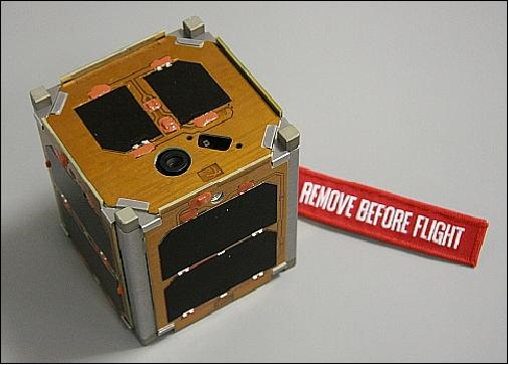
\includegraphics[scale=.9]{fig/ITUpSAT.png}
    \caption[1U sized cubesat ITUpSAT-1]{1U sized cubesat ITUpSAT-1\cite{aslanspace}}
    \label{fig:pSAT}
\end{figure}

In addition to satellites, various research have been performed into individual subsystems such as an interface board, OBC, an EPS and ADCS\cite{aslan2015integration}\cite{karabulut}[\textbf{INTERFACE KARTINA ATIF BUL}]. To date no work have been done regarding the propulsion systems for cube satellites. 

\section{Spacecraft Propulsion Systems}

A propulsion system is defined as a system that enables acceleration for a spacecraft. The contents of this section only includes propulsion systems that are used in space. Other systems such as launch vehicles are not included. 
Propulsion systems may be used to perform variety of tasks in space such as orbital maneuvering, station-keeping or attitude control. 
\par A propulsion system generates thrust, typically expressed in units of newtons(N) that in turn alters the spacecraft's velocity. Thrust is given as the change in momentum with respect to time\cite{goebel2008fundamentals}.

\begin{equation}
    T = \frac{d}{dt}(m_p v_{ex}) = \dot{m}_p v_{ex}
    \label{eq:thrust}
\end{equation}

where $m_p$ is the propellant mass, $v_{ex}$ is the exhaust velocity of the departing propellant and $\dot{m}_p$ is the flow rate of the propellant.


\par In order to examine the performance and propellant usage efficiency of the thruster the term "Specific Impulse" is used, denoted as $I_{sp}$. It is defined as the ratio of the generated thrust to the Earth weight of the flow rate of the propellant as shown in equation \ref{eq:Isp}.
\begin{equation}
    I_{sp} = \frac{T}{\dot{m}_p g}
    \label{eq:Isp}
\end{equation}

Substituting the expression of $\dot{m}_p$ from equation \ref{eq:thrust} into equation \ref{eq:Isp} gives;

\begin{equation}
    I_{sp} = \frac{v_{ex}}{g}
    \label{eq:IspVex}
\end{equation}

Using $v_{ex}$ for specific impulse calculations gives its unit in seconds (s). Higher specific impulse levels means more efficient propellant use. Ion thrusters, part of electric propulsion family, have specific impulse values around 3000 seconds but provide low thrust as opposed to chemical thrusters such as monopropellant thrusters which provide greater thrust at the cost of low specific impulse levels as low as 200 seconds\cite{tsay2009micro}\cite{lemmer2017propulsion}.


\par Based on their operating mechanism propulsion systems can be divided into two main groups as chemical and electric propulsion systems. This section includes general information regarding both types of systems to provide a basis for following sections. 
% Second level titles must be bold and the first letter of each word in the title must be capital (i.e. \textbf{2.1 Process Qualification Analysis}).

% \subsection{Third level title: Only first letter capital}

% Third and fourth level titles must be bold and only the first letter of the word the title begins with must be capital (i.e. \textbf{2.1.1 Process analysis using a histogram} or \textbf{3.1.1.2 Process analysis steps}).

% \subsection{Third level title}

% Third and fourth level titles must be bold and only the first letter of the word the title begins with must be capital (i.e. \textbf{2.1.1 Process analysis using a histogram} or \textbf{3.1.1.2 Process analysis steps}).



% \subsubsection{Fourth level title: Only first letter capital}

% Third and fourth level titles must be bold and only the first letter of the word the title begins with must be capital (i.e. \textbf{2.1.1 Process analysis using a histogram} or \textbf{3.1.1.2 Process analysis steps}).



% \subsubsection{Fourth level title: Only first letter capital}

% Third and fourth level titles must be bold and only the first letter of the word the title begins with must be capital (i.e. \textbf{2.1.1 Process analysis using a histogram} or \textbf{3.1.1.2 Process analysis steps}).

% %{\bf Fifth level title: No numbering after fourth level titles}
% \subsubsubsection{Fifth level title: No numbering after fourth level titles}
\subsection{Chemical propulsion systems}
Chemical propulsion systems exploit the energy in the molecular bonds of the propellant. When the propellant is ignited these molecular bonds are broken and energy is released. Thrust is generated when this hot, expanding propellant is ejected from the spacecraft.
\par Many cube satellites are launched into space as secondary payloads. Limitations of secondary payloads regarding the stored chemicals and combustion within the satellite pose serious challenges. Although there are several systems currently under development, so far no cube satellite with a chemical propulsion system have been launched into space\cite{lemmer2017propulsion}.
%  Depending on the type of the used propellant there are several types of chemical propulsion systems available: monopropellant, bi-propellant and solid rocket engines
% \subsubsection{Monopropellant}
% \subsubsection{Bi-propellant}
% \subsubsection{Solid rocket engines}
\subsection{Electric propulsion systems}
Electric propulsion systems provide thrust by accelerating their propellants. They use the on-board electrical power supply to generate thrust. Compared to chemical propulsion systems they produce less thrust and higher specific impulse\cite{Calik2011}. Due to their low thrust and high specific impulse output they are mainly used for space missions that require high $\Delta$V and propellant usage efficiency. Also due to the low thrust they are often subjected to long continuous use. EP systems can be further examined under three main groups: electrothermal, electrostatic and electromagnetic systems\cite{goebel2008fundamentals}.
\subsubsection{Electrothermal propulsion}

\subsubsubsection{Resistojet Thruster}
Resistojet thrusters constitute the simplest approach for an electric propulsion system. Compressed propellant, either in liquid or gas state, is fed into the nozzle of the thruster. Within the nozzle area is located a heating element. This heating element is usually just a simple resistor that produce ohmic heating due to current flow. As the propellant passes through the heating area it heats up and expands. This expanded gas is then ejected from the spacecraft to produce thrust. A schematic of a resistojet thruster is shown in figure \ref{fig:resistojet}

\begin{figure}[ht]
    \centering
    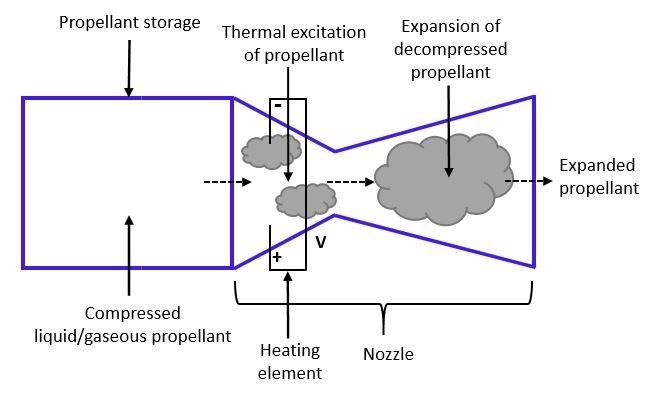
\includegraphics[scale=0.65]{fig/resistojet.png}
    \caption[Resistojet thruster schematic]{Resistojet thruster schematic\cite{tummala2017overview}}
    \label{fig:resistojet}
\end{figure}

Even though they have a considerable flight heritage on regular sized satellites none have flown into space on board a cube satellite so far\cite{lemmer2017propulsion}. Several companies have developed or in the process of developing resistojet thrusters. CubeSat High Impulse Propulsion System(CHIPS) designed and developed by CU Aerospace is stated to provide specific impulse of 76 s and thrust of 31 mN with 25W of power consumption\cite{hejmanowski2015cubesat}. Busek company has developed a micro resistojet thruster that can provide 150s specific impulse and 30 mN at 15W input power\cite{lemmer2017propulsion}. Both of these designs share similar sizes and occupy approximately 1U volume. 
\par Resistojet thrusters suffer from low efficiency obvious by their low specific impulse values. However considering their low power consumption and high thrust output they may be suitable for cubesat missions.

\subsubsubsection{Arcjet Thruster}

Similar to resistojets the aim of an arcjet thruster is to heat up the propellant and then eject the expanding propellant to create thrust. The method of heating up the propellant however, is different. Instead of a heating element an arcjet thruster consists of an anode, acentral cathode and injector. Prior the ignition high voltage, on the level of thousands of volts, is applied in between the cathode and anode. Ignition and arc forming occurs due to paschen-discharge\cite{wadhwa2006high} in the gap between the anode and cathode. Propellant injected into this gap is heated up and expanded. Expanded propellant is directed into the nozzle and thrust is generated. Working principle of an arcjet thruster is illustrated in figure \ref{fig:arcjet}

\begin{figure}[htb]
    \centering
    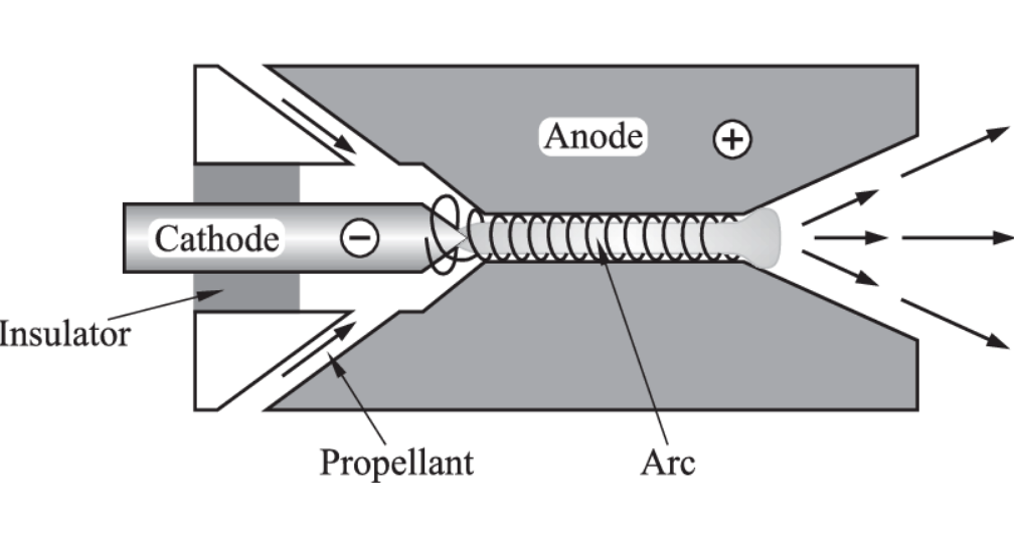
\includegraphics[scale=0.65]{fig/arcjet.png}
    \caption[Arcjet thruster schematic]{Arcjet thruster schematic\cite{bock2011electric}}
    \label{fig:arcjet}
\end{figure}

Plasma effects that occur because of the high current arc is neglectible since propellant is only weakly ionized. Specific impulse provided by the arcjets are recorded to be limited at approximately 700 s\cite{goebel2008fundamentals}.

\subsubsection{Electrostatic propulsion}
\subsubsubsection{Ion Thruster}
Ion thrusters, or sometimes called ion engines, utilize ions to create thrusts. These ions are supplied by the plasma generated and sustained within the thruster. In order to accelerate the ions a grid extraction system is used. This extraction system consists of two or three biased grids that create an electrostatic field. Any ion that encounters this electrostatic field is then ejected from the spacecraft. Depending on the mass of the used propellant ejected ions can reach speeds up to 1000 km/s\cite{goebel2008fundamentals}. They can provide $I_{sp}$ values up to 3500 s\cite{Calik2011}. Since spraying only ions from spacecraft will cause spacecraft be rapidly charged a neutralizer mechanism is needed to preserve the neutrality of the spacecraft.
\par There are three main types of ion thrusters in literature. First one is called Kaufman type thruster, also known as electron bombardment thruster, mainly studied in the United States, another one is RF ion thruster originated and predominantly studied in Germany and lastly Microwave or Electron-Cyclotron Resonance(ECR) thruster studied in Japan\cite{kokal2017design}\cite{OCW1964}\cite{Bumbarger}.
. Main difference between mentioned types of ion thrusters is their individual methods to create and sustain plasma. All subtypes of ion thrusters share the same ion acceleration mechanism. 

\par Working schematic of a Kaufman or electron bombardment ion thruster is shown in figure \ref{fig:kaufman}.

\begin{figure}[ht]
    \centering
    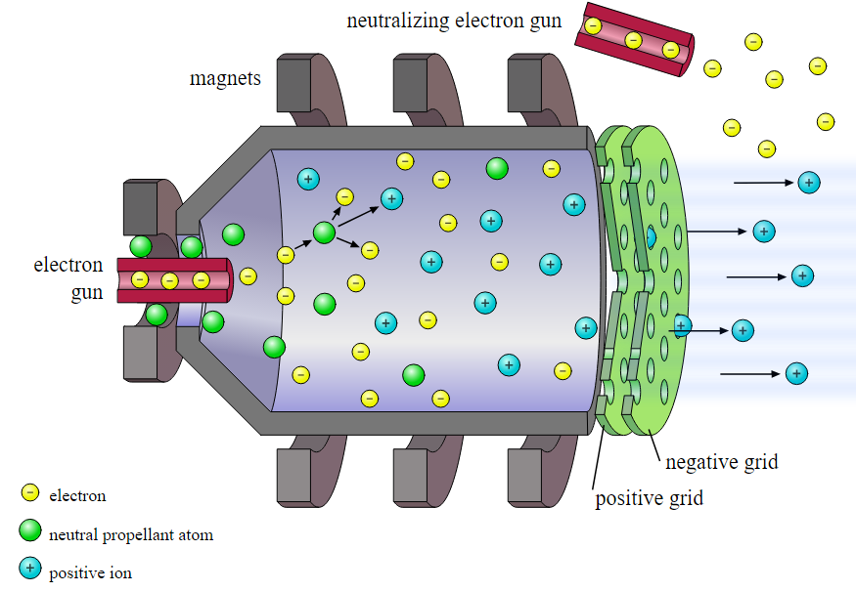
\includegraphics[scale=0.9]{fig/kaufman.png}
    \caption[Kaufman type ion thruster schematic]{Kaufman type ion thruster schematic\cite{kaufman}}
    \label{fig:kaufman}
\end{figure}

Electrons needed to ignite the plasma are pumped via an electron gun into the cylindirical discharge chamber. From same location neutral propellant is also fed into the chamber. Energetic electrons from electron gun collide with neutral propellant atoms and suffer elastic collisions. Through these collisions a valance electron from the neutral propellant atoms is ripped off. As a result an electron and an ion is obtained from the neutral atom in addition to the initial colliding electron. Energy acquired from the broken bond and presence of ions ignite the plasma and chain reaction resulting from increased density of electrons in the enviroment sustain the plasma\cite{goebel2008fundamentals}.
\par A pair of grids are located at the end of discharge chamber. Grid closer to the plasma is named as screen grid and is positively biased wheras the grid positioned away from the plasma is positively biased and named as acceleration grid. Electrostatic field created by the pair of grids accelerate the ions present in the plasma and create thrust\cite{kokal2017design}. Accelerated ions form an ion beam at the downstream of accelerator grids. Remaining electrons inside the plasma are drawn to walls which act as anodes. Magnets are used to create suitable magnetic fields to increase the amount of time electrons spend in the discharge chamber before evacuated to the anode and thus increase the chance of plasma ignition\cite{OCW1964}.
\par Same amount of electron density received at the anode walls of the thruster is injected into the extracted ion beam in order to keep the spacecraft neutral.

For RF ion thruster the plasma is formed by using a helical antenna wrapped around the discharge chamber. A diagram of such device is shown in figure \ref{fig:rfschematic}.

\begin{figure}[ht]
    \centering
    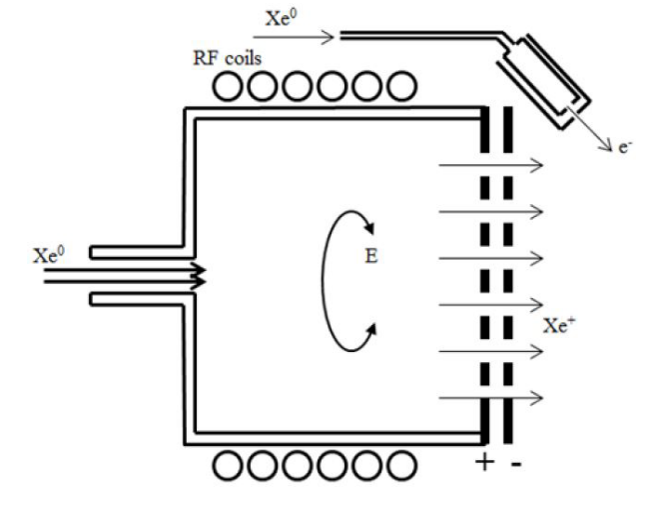
\includegraphics[scale=0.75]{fig/rfschematic.png}
    \caption[RF Ion Thruster Schematic]{RF Ion Thruster Schematic\cite{kokal2017design}}
    \label{fig:rfschematic}
\end{figure}

RF ion thrusters are cathodeless designs. Free electrons needed for plasma ignition can be retrieved from the neutralizer thruster chamber by reverse polarizing the grids. When an RF signal is broadcasted to the discharge chamber it acts as a solenoid and creates an axial magnetic field and perpendicular azimuthal electric field. Electrons inside the chamber start to display a tangential motion within the chamber under the influence of broadcasted signal and get energized. At this point a propellant is introduced to the discharge chamber. Electrons with high energy inside plasma collide with neutral propellant atoms and create a plasma. Depending on the power levels supplied by the RF antenna the resulting plasma can either be low density capacitively coupled plasma(CCP) or high density inductively coupled plasma(ICP). In CCP mode voltage from the helical coil is capacitively coupled to the chamber walls and create strong enough electric field to break down the propellant\cite{farnell2007performance}. During the ICP mode RF energy is coupled to the free electrons through magnetic induction\cite{Bumbarger}. RF signal is typically in the range of 1-13.56MHz\cite{mistoco2004development}.
The same two or three grid accelerator system used in Kaufman thrusters is used to accelerate and eject the ions from the device to create thrust. Main advantages of the RF ion thruster is that it utilizes a simple design and the helical coil is not in contact with plasma and thus have a longer life time. 

Electron-Cyclotron Resonance (ECR) thrusters utilize high frequcency (>1GHz) microwave(MW) signals to create a free floating plasma and heat the propellant. Working schematic is shown in figure \ref{fig:ecrschematic}.

\begin{figure}[ht]
    \centering
    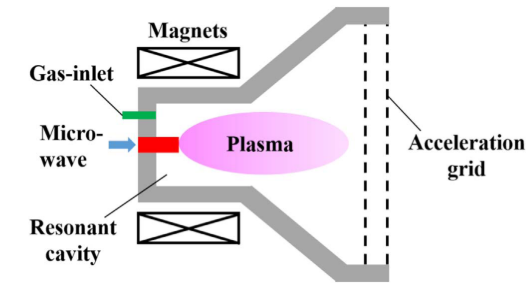
\includegraphics[scale=0.75]{fig/ecr.png}
    \caption[Schematic of ECR Thruster]{Schematic of ECR Thruster\cite{xiaogang2020heating}}
    \label{fig:ecrschematic}
\end{figure}

In a ECR microwave signals are broadcasted into the resonance cavity and a standing wave is formed. Free electrons present in the enviroment and propellant are coupled to the electric field and become ionized. These energetic electrons then collide with neutral propellant atoms to create a plasma similar to other types of ion thrusters. Once the plasma is ignited in the cavity region it can sustain itself by producing more free electrons and collisions. 

Main propellant type for ion thrusters are noble gasses such as Xenon, Krypton, Argon. Some non-noble gasses such as Mercury or Iodine have been used as well. Noble gasses are chemically inert and thus are safe to store. In addition they pose no risk of contamination for sensitive spacecraft surfaces such as solar panels or optics. Xenon have been predominantly used in electric propulsion purposes due to its high atomic mass (131amu) and higher thrust output but it requires more power to accelerate heavier Xenon when compared to other types of noble gasses. In addition Xenon is considerably expensive. Other types of noble gasses such as Argon or Krypton have gained popularity. With atomic masses of 39 amu and 83 amu for Argon and Krypton respectively they provide less thrust than Xenon but their wide availabilty make them more appealing\cite{Calik2011}. 




\subsubsubsection{Hall Thruster}
Hall thrusters, like ion engines, use ions to create thrusts. They employ magnetic circuits to trap electrons and collide trapped electrons with neutral propellant to create ions. Created ions are expelled from the thruster by utilizing the electric field created by the same magnetic circuit used to trap the electrons. A working schematic of a typical hall thruster is shown in figure \ref{fig:HET}.

\begin{figure}[ht]
    \centering
    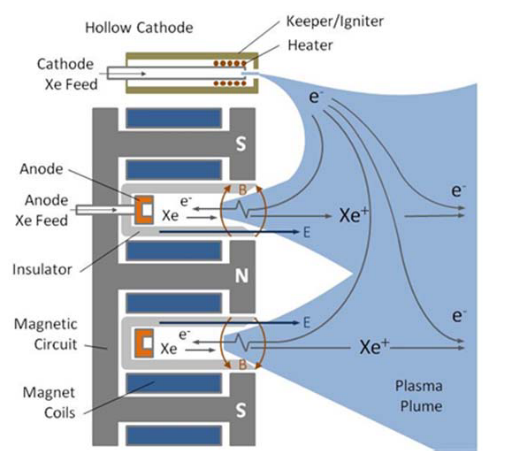
\includegraphics[scale=0.75]{fig/HET.png}
    \caption[Schematic of Hall Effect Thruster]{Schematic of Hall Effect Thruster\cite{szabo2020one}}
    \label{fig:HET}
\end{figure}

An electron source, in the case of figure \ref{fig:HET} a hollow cathode, is used to provide electrons. An anode is used to attract the electrons to the annular channel within the thruster. Once electrons are within the channel they are trapped due to radial magnetic fields created by specifically located magnetic circuits. Electrons inside the channel begin to exhibit tangential motion around the thruster axial axis. During this motion they incur a current called Hall current, hence the thruster's name. A neutral propellant is injected into the channel. Propellant atoms collide with energetic electrons inside channel and are ionized. Created ions are accelerated and subsequently ejected from the thruster by an axial electric field, perpendicular to the magnetic field created by the magnetic circuit. Some of the electrons originated from the cathode is used to neutralize the created ion beam. 

\par They contain a simple design compared to ion engines but magnetic and electric fields needs to be optimized to provide an efficient operation. Their $I_{sp}$ and efficiency values are somewhat less than other types of electorstatic propulsion systems but their thrust levels are significantly higher\cite{goebel2008fundamentals}. 

% \subsubsubsection{Field Emmission Electric Propulsion(FEEP) Thruster}


\subsubsection{Electromagnetic propulsion}

\subsubsubsection{Pulsed Plasma Thruster (PPT)}
Capacitors and spark igniters are used to create a discharge through a series of impulse bits. Solid, liquid or gas propellant can be used. If the used propellant is solid then this discharge ablates and removes small parts of the propellant. Same discharge also partially ionizes the propellant. Ionized propellant is then accelerated by Lorentz forces\cite{lemmer2017propulsion}. 
\par PTFE is traditionally used as solid propellant\cite{yost2021state}. Thrust levels are limited to the frequency of the charged capacitor. Spark igniter can limit the lifetime of the thruster. Their advantage is low power use. They can generate moderately high $I_{sp}$ values up to 800 s with 80$\mu$N with only 10W of power\cite{Calik2011}.

\subsubsubsection{Magnetoplasmadynamic (MPD) Thruster}
In MPD thrusters a propellant is ionized by using arcs generated by high currents. Ionized propellant is accelerated by electromagnetic forces such as Lorentz force to generate thrust. Since Lorentz force $J\times B$, where J is the current density and B is the magnetic flux density, utilize both current and magnetic field MDP's require greater power compared to other types of electric propulsion systems. At the same time they provide higher thrust (>1N) and higher $I_{sp}$ values (>5000 s)\cite{zheng2021integrated}. Working schematic of an MPD is shown in figure \ref{fig:MPD}

\begin{figure}[ht]
    \centering
    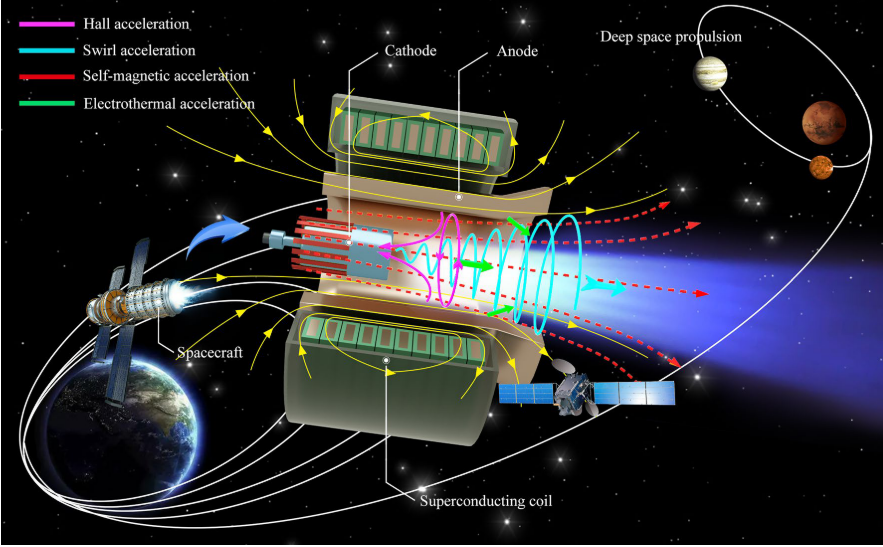
\includegraphics[scale=0.6]{fig/MPD.png}
    \caption[Working principle of a MPD thruster]{Working principle of a MPD thruster\cite{zheng2021integrated}}
    \label{fig:MPD}
\end{figure}

\newpage

\section{Thesis Purpose and Overview}\label{purposeofthesis}
Cube satellites offer very limited power budgets and volume limitations due to their small sizes. For an electric propulsion system to work properly it should be both compact and power efficient. Considering these factors for this thesis study an RF ion thruster is selected to be built. [\textbf{DÜZELT}]
RF ion thrusters do not include complex parts such as an electron source or magnets to confine the plasma. Their design simply consists of a plasma generator; an RF antenna wrapped around a discharge chamber and a pair of biased grids. Regardless of their simplicity they offer the highest $I_{sp}$ among the electric propulsion systems and are renowned for their scalability\cite{tsay2016maturation}. 
Another reason for RF ion thruster choice is the significant accumulation of know-how regarding their structure and testing at Bogazici University Space Technologies Laboratory(BUSTLab). Testing equipment within the BUSTLab such as the vacuum chamber, DC power sources, matching network tuner and RF signal generator are best suited for RF ion thruster operations\cite{yavuz2013prototype}.  
                                       
%%%%%%%%%%%%%%%%%%%%%%%%%%%%%%%%%%%%%%%%%%%%%%%%%%%%%%%%%%%%%%%%%
\chapter{BACKGROUND}\label{ch:2_background}
%%%%%%%%%%%%%%%%%%%%%%%%%%%%%%%%%%%%%%%%%%%%%%%%%%%%%%%%%%%%%%%%%
\vspace*{-12pt} % If no text above section, use this vspace* to lift the whole part to the proper starting point - SBÖ
\section{Basic Plasma \& RF Thruster Physics}\label{ChBasicPlasma}
RF ion thruster accelerates charged particles called ions up to 40 km/s to produce thrust\cite{goebel2008fundamentals}. Accelerated ions are sourced from the plasma generated and sustained within the thruster. Before elaborating further on the thruster systems a basic understanding of plasma physics is required. 

\par Plasma is defined as combination of positively charged ions, negatively charged electrons and neutral particles. Densities of charged ions and electrons are assumed equal. This equilibrium state is referred as "quasi-neutrality"\cite{Calik2011}. Thus on a macroscopic scale plasma is considered to be charged neutrally. 
This neutral state is violated under two conditions. One of the conditions is when the plasma is studied near its boundary regions. In such regions due to interaction with the thruster walls a \textit{sheath} is formed in which the densities of positively and negatively charged particles vary.
Second condition occurs when the plasma is examined in microscopic scales. In microscopic scales there are regions in which the neutrality is broken\cite{lieberman2005principles}. The size of such regions are approximated by a certain lenght called \textit{Debye length}.  Effects of plasma sheaths, their occurance and relation to Debye length will be discussed in chapter \ref{ch:sheaths}. 

\par Since plasma has a certain amount of electric charge it can be affected by magnetic and electrical forces\cite{Couch2017}. General behaviour of electric and magnetic fields generated by plasma acts in compliance with Maxwell's equations which are provided in equations \ref{eq:maxwell1} \cite{griffiths2005introduction}.

\begin{equation}
    \begin{aligned}  
    \nabla \cdot \mathbf{E} = \frac{\rho}{\epsilon_0} \\
    \nabla \cdot \mathbf{B} = 0 \\
    \nabla \times \mathbf{E} = - \frac{\partial B}{\partial t} \\
    \nabla \times \mathbf{B} = \mu_0 \left(\textbf{J}+\epsilon_0 \frac{\partial \mathbf{E}}{\partial t}\right)
\end{aligned}
\label{eq:maxwell1}
\end{equation}


In which \textbf{E} is the electric field vector, \textbf{B} is the magnetic flux vector, $\rho$ is the plasma charge density, $\epsilon_0$ and $\mu_0$ are permittivity and permeability of vacuum respectively and \textbf{J} is the current density\cite{goebel2008fundamentals}. Plasma charge density $\rho$ is defined as;
\begin{equation}
    \rho = \sum_{n} q_s n_s = e (Z n_i - n_e)
    \label{eq:plasmacharge}
\end{equation}

where $q_s$ is the charge state and $n_s$ is the number density of an arbitrary species named \textit{s}. e is the electron charge, Z is the charge state, $n_i$ is the ion density, $n_e$ is the electron density. Current charge density \textbf{J} is formulated by the equation\cite{goebel2008fundamentals};

\begin{equation}
    J = \sum_{s} q_s n_s \upsilon_s = e (Z n_i \upsilon_i - n_e \upsilon_e)
    \label{eq:currentchargedensity}
\end{equation}

in which $\upsilon_s$, $\upsilon_i$ and $\upsilon_e$ are the velocities of the species \textit{s}, the ion and the electron, respectively. Electric field \textbf{E} occuring in the ion thrusters is given as\cite{Couch2017};

\begin{equation}
    \mathbf{E} = - \nabla \varPhi 
\end{equation}

where $\varPhi$ is the electric potential.
%  Value of \textbf{E} is negative since \textbf{E} always points in the direction of motion.  

\par Motion of a charged particle within the thruster can be described by equation \ref{eq:lorentz}
\begin{equation}
    \mathbf{F} = m\frac{d\mathbf{v}}{dt} = q(\mathbf{E}+\upsilon \times \mathbf{B})
    \label{eq:lorentz}
\end{equation}

Which is defined as the Lorentz force equation\cite{goebel2008fundamentals}. In the case of magnetic field \textbf{B} in axial direction of the thruster with no electric field \textbf{E} the motion of particles can be found from equation \ref{eq:lorentz}.

\begin{equation}
    \begin{aligned}  
m\frac{\partial v_x}{\partial t} = q B v_y \\
m\frac{\partial v_y}{\partial t} = -q B v_x \\
m\frac{\partial v_z}{\partial t} = 0 \\
\end{aligned}
\label{eq:lorentzxdir}
\end{equation}

Taking one more time derivative of equation \ref{eq:lorentzxdir} results;

\begin{equation}
    \begin{aligned}
        a = \frac{\partial^2 v_x}{\partial t^2} = \frac{qB}{m}\frac{\partial v_y}{\partial t} \\
        a = \frac{\partial^2 v_y}{\partial t^2} = -\frac{qB}{m}\frac{\partial v_x}{\partial t}
    \end{aligned}
    \label{eq:lorentzxdir2}
\end{equation}

Substituting partial time derivative values from equation \ref{eq:lorentzxdir} into equation \ref{eq:lorentzxdir2} yields;

\begin{equation}
    \begin{aligned}
        \frac{\partial^2 v_x}{\partial t^2} = - \left(\frac{qB}{m}\right)^2 v_x \\
        \frac{\partial^2 v_y}{\partial t^2} = - \left(\frac{qB}{m}\right)^2 v_y
    \end{aligned}
    \label{eq:lorentxdir3}
\end{equation}

Equation \ref{eq:lorentxdir3} shows that particle displays a harmonic oscillation with a certain frequency defined as cyclotron frequency $\omega_c$;

\begin{equation}
    \omega_c = \frac{qB}{m}
    \label{eq:cyclotronfreq}
\end{equation}


% Reassembling the equations at equation \ref{eq:lorentzxdir} gives

% \begin{equation}
%     \frac{m}{qB}\frac{\partial v_x}{\partial t} = v_y
% \end{equation}

% The part $\dfrac{qB}{m}$ is defined as cyclotron frequency and denoted as $w_c$.

% Integrating the equation \ref{eq:lorentzxdir} once for velocity and twice for position vectors yield\cite{lara2016design};

% \begin{equation}
%     \begin{aligned}
%         v_x = \frac{q}{|q|}v_n sin(w_c t + \varphi ) \\
%         v_y = -\frac{q}{|q|}v_n cos(w_c t + \varphi)
%     \end{aligned}
%     \label{eq:velvectors}
% \end{equation}

% \begin{equation}
%     \begin{aligned}
%         x = \frac{v_n}{w_c}cos(w_c t + \varphi) \\
%         y = \frac{v_n}{w_c}sin(w_c t + \varphi) \\
%     \end{aligned}
%     \label{eq:posvectors}
% \end{equation}

% From equations \ref{eq:velvectors} and \ref{eq:posvectors} it can be seen that the particle performs a circular motion within the magnetic field with a constant velocity $v_n$ and cyclotron frequency $w_c$.
 Orbit size of this circular motion can be found by observing this circular motion displayed in figure \ref{fig:larmor}.

\begin{figure}[ht]
    \centering
    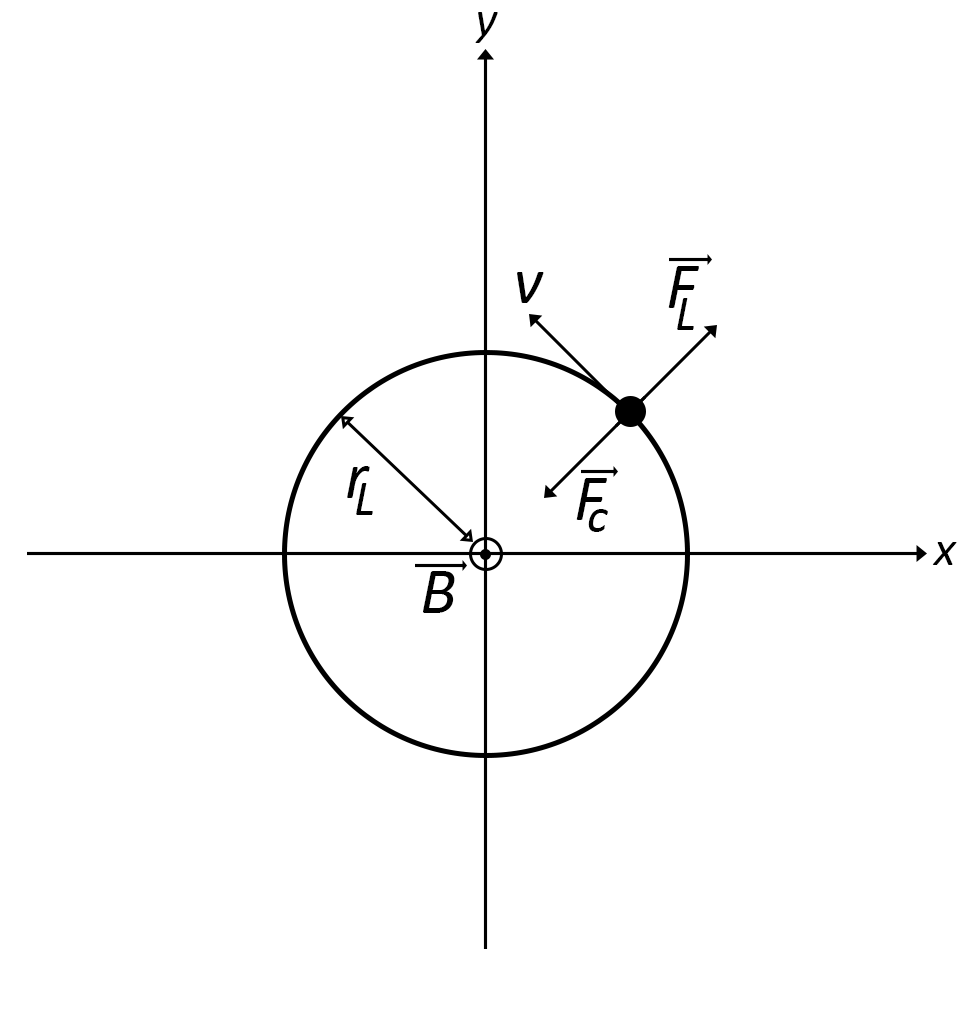
\includegraphics[scale=0.25]{fig/larmor.png}
    \caption{Motion of a particle in a uniform axial magnetic field}
    % {Motion of a particle in a uniform axial magnetic field\cite{lara2016design}}
    \label{fig:larmor}
\end{figure}

Charged particle shown in figure \ref{fig:larmor} will act under the influence of a Lorentz force;
\begin{equation}
    \mathbf{F} = q\mathbf{v} \times \mathbf{B}
    \label{eq:circularlorentz}
\end{equation}

Same particle will also feel a centripetal force;
\begin{equation}
    \mathbf{F_c} = \frac{mv^2}{r_L}
    \label{eq:centripetal}
\end{equation}

For a constant uniform motion equations \ref{eq:circularlorentz} and \ref{eq:centripetal} must be equal.

\begin{equation}
    q\mathbf{v} \times \mathbf{B} = \frac{mv^2}{r_L}
    \label{eq:larmor}
\end{equation}

where $r_L$ is the \textit{Larmor radius} and is the radius of the particle's circular motions shown in equation \ref{eq:larmorradi}
\begin{equation}
    r_L = \dfrac{mv}{qB}
    \label{eq:larmorradi}
\end{equation}


% Same magnetic field \textbf{B} also creates an electric field \textbf{E}. Direction of this electric field is perpendicular to the magnetic field. If the direction of the magnetic field is assumed as axial then the electric field direction becomes tangential. 

% \par There are different types of plasma that occur on low pressure enviroment; DC glow discharge, capacitively coupled plasma(CCP) and inductively coupled plasma(ICP)


% \begin{equation}

%     \label{eq:lorentzydir}
% \end{equation}

% \begin{equation}

%     \label{eq:lorentzzdir}
% \end{equation}

% where $\upsilon$ is particle velocity and \textbf{F} is thrust. Since energetic electrons inside the ion thruster act mainly under the influence of the electric field other elements of equation \ref{eq:lorentz} can be omitted\cite{goebel2008fundamentals}. Rewriting equation \ref{eq:lorentz} can simply be rewritten;

% \begin{equation}
%     \mathbf{F} = q\mathbf{E}
%     \label{eq:lorentzsimple}
% \end{equation}

% Assuming a Maxwellian distribution among the particles average three dimensional kinetic energy and particle speed equations can be expressed as\cite{griffiths2005introduction};

% \begin{equation}
%     E_{avg} = \frac{3}{2}kT
% \end{equation}

% \begin{equation}
%     \overline{\upsilon} = \sqrt{\left(\frac{2kT}{\pi m}\right)}
% \end{equation}

% where m is the mass of particle, k is Boltzmann's constant and T is the temperature. 

\subsection{Sheats at The Boundaries of The Plasma} \label{ch:sheaths}

Earlier in the chapter \ref{ChBasicPlasma} it was mentioned that the quasi-neutral stance of the plasma is broken along the plasma boundary in regions called sheaths. Since ion acceleration grids exploit the sheath at the edge of the plasma a solid understanding of sheath behavior is very important to model and design an ion thruster.

After the initial ignition of plasma created ions and free electrons will be lost due to interaction with the containing walls. Since electrons have much higher velocities compared to ions they will exit the plasma in larger quantities. Over time this imbalance creates a negatively biased container walls with respect to the plasma. This negative charge attracts ions from the plasma and repel the electrons, causing a non-neutral region on the border of plasma. This region in which the plasma loses its neutrality is called sheath\cite{lara2016design}.

\begin{figure}[ht]
    \centering
    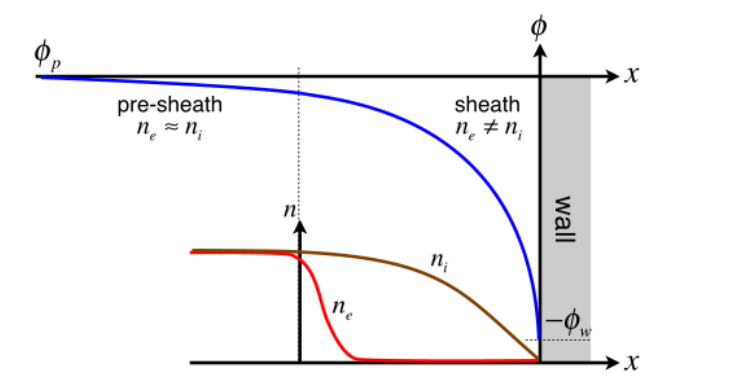
\includegraphics[scale=0.75]{fig/sheath.png}
    \caption[Potential and species density change near plasma boundary]{Potential and species density change near plasma boundary\cite{lara2016design}}
    \label{fig:sheathgraph}
\end{figure}
\newpage
Figure \ref{fig:sheathgraph} shows how the species densities and potential is changing while approaching the plasma boundary. As particles get close to the wall negative potential $-\phi_w$ attracts ions and repels electrons causing a charge inbalance. The thickness of this sheath region is given in the order of Debye lenght $\lambda_D$\cite{goebel2008fundamentals}. Thanks to the shield that occurs the remainder of plasma maintains its potential $\phi_p$. 

% If the potential throughout the sheath is too large compared to the electron temperature a sheath forms. If this potential is large enough the electrons are repelled away from the plasma. Under these circumstances the electron density in the regions around the sheath edge is close to zero. 

% \begin{equation}
%     J = \frac{4 \epsilon_0}{9}\sqrt{\frac{2e}{M}}\frac{V^{\frac{3}{2}}}{l_e^2}
%     \label{eq:childlangmuir}
% \end{equation}

% The result gives J, current density or current per unit area. In equation \ref{eq:childlangmuir} M is the mass of the particle, V is the voltage and $l_e$ is the sheath thickness which can be calculated by using the following formula\cite{williams2013ion};

% \begin{equation}
%     l_e = \sqrt{(l_g + t_s)^2+\frac{d_s^2}{4}}
%     \label{eq:sheaththickness}
% \end{equation}

% where $l_g$ is the distance between grids, $t_s$ is the screen grid thickness and $d_s$ is the diameter of one aperture of the screen grid. Representations of the same parameters can also be seen in figure \ref{fig:sheaththickness}.
% \newpage

% \begin{figure}[ht]
%     \centering
%     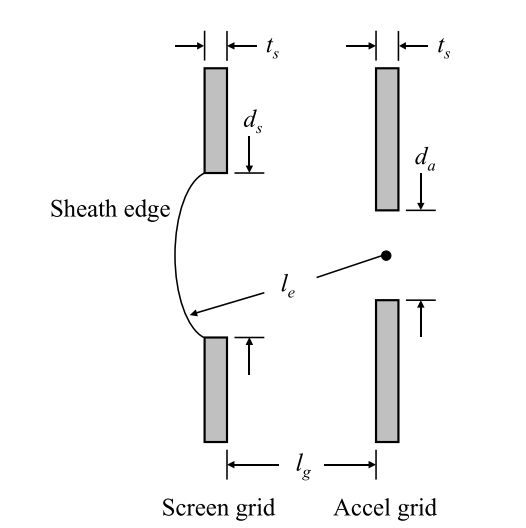
\includegraphics[scale=0.75]{fig/sheaththickness_toddwilliams.png}
%     \caption[Sheath forming representation between grids]{Sheath forming representation between grids\cite{williams2013ion}}
%     \label{fig:sheaththickness}
% \end{figure}




% \section{Rocket Equation For RF Ion Thrusters}

\section{General RF Ion Thruster Design Parameters} \label{ch:generaldesign}

General design of RF ion thruster was shown in figure \ref{fig:rfschematic}. This figure will be examined by dividing the figure into two main regions. One of these regions is where the plasma ignition occurs and the other is where the ion extraction and ejection are performed. \\
Within the thruster the plasma is ignited and sustained within the discharge chamber.  Propellant is fed into the discharge chamber. Plasma is then created by means of an RF coil wrapped around the discharge chamber. An RF signal is put through this coil creates an electromagnetic field within the discharge chamber and ignites the plasma. During operation coil does not come into contact with the plasma. Both RF coil and the discharge chamber constitute the plasma ignition region.
Created quasi-neutral plasma interacts with a pair of grids placed at the exit of the discharge chamber. This pair of grids make up the ion extraction and ejection region. By oppositely polarizing the grids an electrostatic field is created which extract and ejects the ions. \\
Parameters regarding the design of discharge chamber, RF coil and ion extraction grids affect the thrust and specific impulse values of the thrusters. They will be examined individually in the following subsections. 
\subsection{Discharge Chamber and RF Coil}

Plasma is created and sustained in discharge chamber. As a result most of plasma-surface interaction occurs within the discharge chamber. Energetic particles, both ions and electrons, are
lost to the discharge chamber walls. Initial RF ion thruster designs included cylindrical discharge chambers in order to ease the RF coil placement. An example of this cylindirical design can be seen in figure \ref{fig:RIT2}. 
\newpage
\begin{figure}[ht]
    \centering
    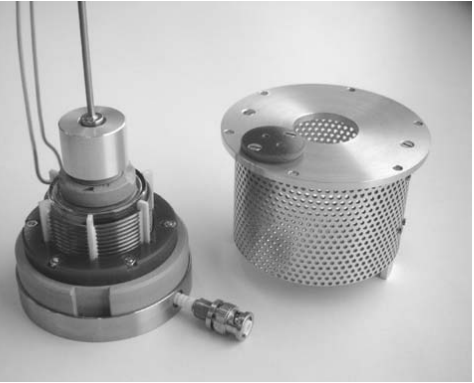
\includegraphics[scale=0.8]{fig/RIT2.png}
    \caption[Disassembled model of RIT-2 developed by Giessen University]{Disassembled model of RIT-2 developed by Giessen University\cite{loeb2004development}}
    \label{fig:RIT2}
\end{figure}

In the figure \ref{fig:RIT2} discharge chamber is shown at the left side, wrapped by a coil. Length of the coil depends on the length of the discharge chamber. If the discharge chamber is long 
then more antenna can be accomodated which in turn creates more induction. But as a downside longer discharge chamber means longer particle loss area for the plasma. Research have been conducted to reduce the particle loss area without drastically altering the coil. As a result conical and hemispherical discharge chambers have been devised. Examples for conical and hemispherical discharge chamber designs can be seen in figures \ref{fig:RITXT} and \ref{fig:RIT45} respectively

\begin{figure}[ht]
    \centering
    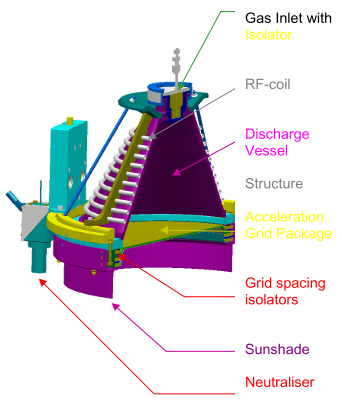
\includegraphics[scale=0.75]{fig/RITXT.png}
    \caption[Cutaway drawing of RIT-XT thruster highlighting conical design]{Cutaway drawing of RIT-XT thruster highlighting conical design\cite{leiter2003development}}
    \label{fig:RITXT}
\end{figure}
\newpage
\begin{figure}[ht]
    \centering
    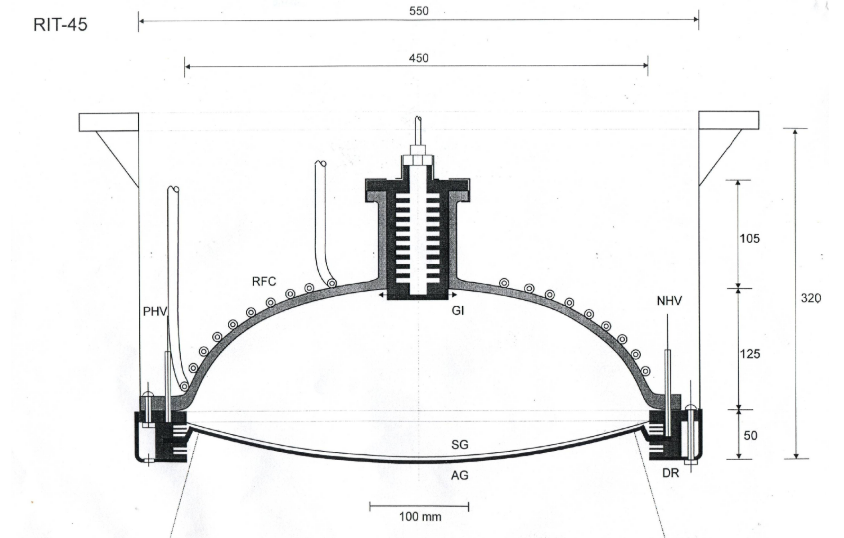
\includegraphics[scale=.6]{fig/RIT45.png}
    \caption[Hemispherical discharge chamber schematic of RIT-45]{Hemispherical discharge chamber schematic of RIT-45\cite{loeb2011design}}
    \label{fig:RIT45}
\end{figure}

Since RF coil is located at the outside of the discharge chamber, RF signals have to be able to easily penetrate the chamber walls in order to form electromagnetic fields inside the chamber. Since an electrical conductive material would act as a Faraday cage and keep RF signals from penetrating, the material of discharge chamber has to be non-conductive. Non-conductive and thermally durable materials such as quartz or alumuna have been common choices for discharge chamber material\cite{goebel2008fundamentals}. \\
RF coil is made of a highly conductive material such as copper. An example of RF coil is shown in figure \ref{fig:coppercoil}

\begin{figure}[ht]
    \centering
    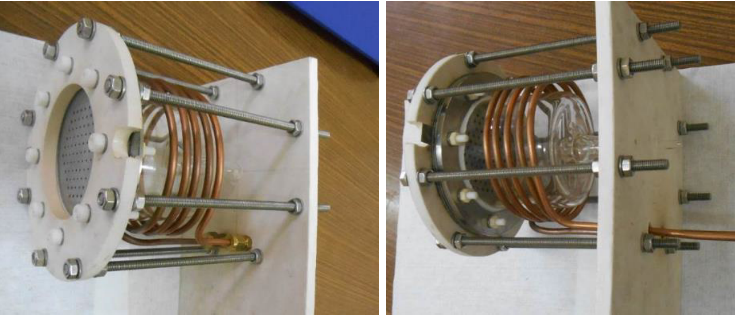
\includegraphics[scale=.75]{fig/burfitcoil.png}
    \caption[Copper coil wrapped around BURFIT-80 thruster]{Copper coil wrapped around BURFIT-80 thruster\cite{kokal2017design}}
    \label{fig:coppercoil}
\end{figure}
\newpage

Another RF antenna configuration is planar antenna. In this configuration RF antenna is placed at the base of discharge chamber as shown in figure \ref{fig:planarantenna}.
\begin{figure}[ht]
    \centering
    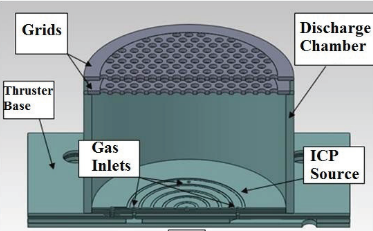
\includegraphics{fig/planarantenna.png}
    \caption[Planar antenna, denoted as ICP source, placed at the base of discharge chamber]{Planar antenna, denoted as ICP source, placed at the base of discharge chamber\cite{Bumbarger}}
\label{fig:planarantenna}
\end{figure}

Planar antenna configuration results in high-density and more uniform plasma discharge compared to wrapped RF coil configurations. This configuration is ideal since the area around the 
discharge chamber remains empty and can accomodate other optional thruster elements such as magnets for plasma containment. Since focus of this work is simplicity and scalability of ion thrusters there 
will be no magnets present. This situation also negates the need for a planar RF antenna configuration\cite{gillman2008low}. 

Frequency of broadcasted signal through RF coil is important.  Literature survey reveals that for optimal power transfer from coil to plasma, broadcasted signal frequency should be half of particle collision frequency\cite{holste2018performance}. In typical thrusters RF frequency is kept in the order of 1MHz\cite{goebel2008analytical}. In this work however RF signal frequency will be 13.56 MHz which is an industrial-scientific-medical standard. RF power supply that will be used in this work is originally designed for industrial processes such as plasma etching. For this work the power supply will be repurposed to fit RF ion thruster operations. 

Inductivity of the coil is directly related to the number of turns it makes around the discharge chamber. High turn number means higher inductivity however it also means longer coil. Longer coil will waste more power due to ohmic losses\cite{tsay2012micro}. In order to reach an optimal level a trade-off has to be made. 

\subsection{Ion Extraction Grids}
Ion extraction is performed by a group of aligned grids. They are placed in tandem to each other as shown in the schematic at figure \ref{fig:rfschematic}. Grid located closer to the plasma is named \textit{screen} grid whereas the grid located away from the plasma is called \textit{accelerator} grid. These grids contain numerous apertures in them as shown in figures \ref{fig:burfitscreen} and \ref{fig:burfitscreen}. 

\begin{figure}[ht]
    \centering
    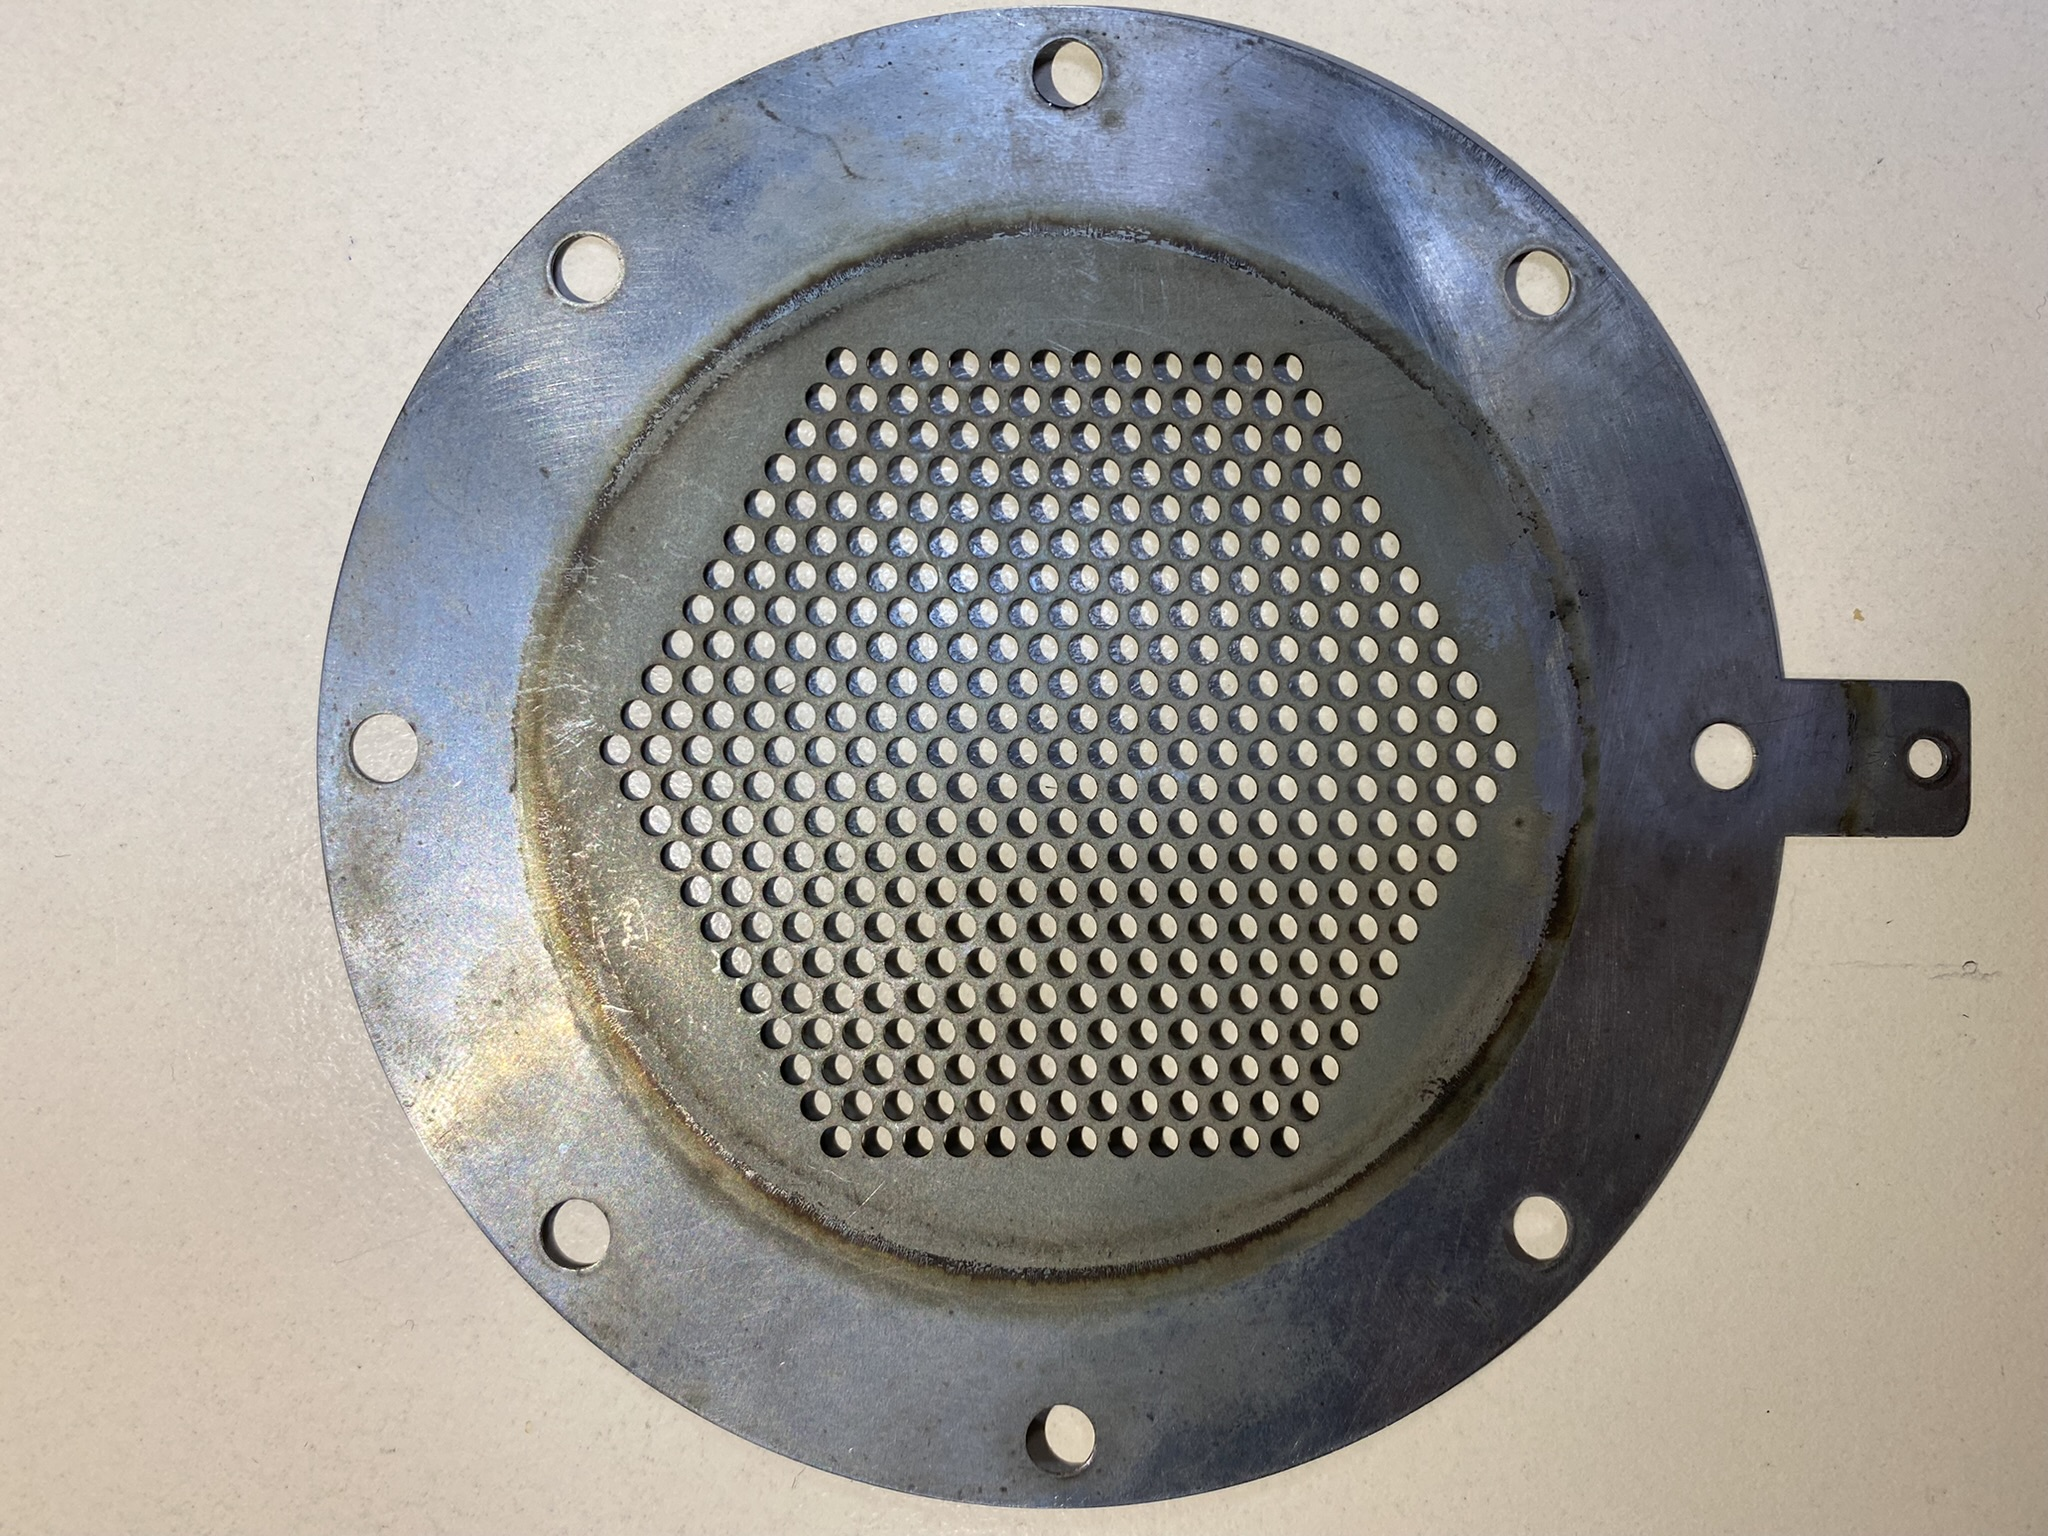
\includegraphics[scale=0.15]{fig/screen.jpeg}
    \caption{Screen grid of BURFIT-80}
    \label{fig:burfitscreen}
\end{figure}
\newpage
\begin{figure}[ht]
    \centering
    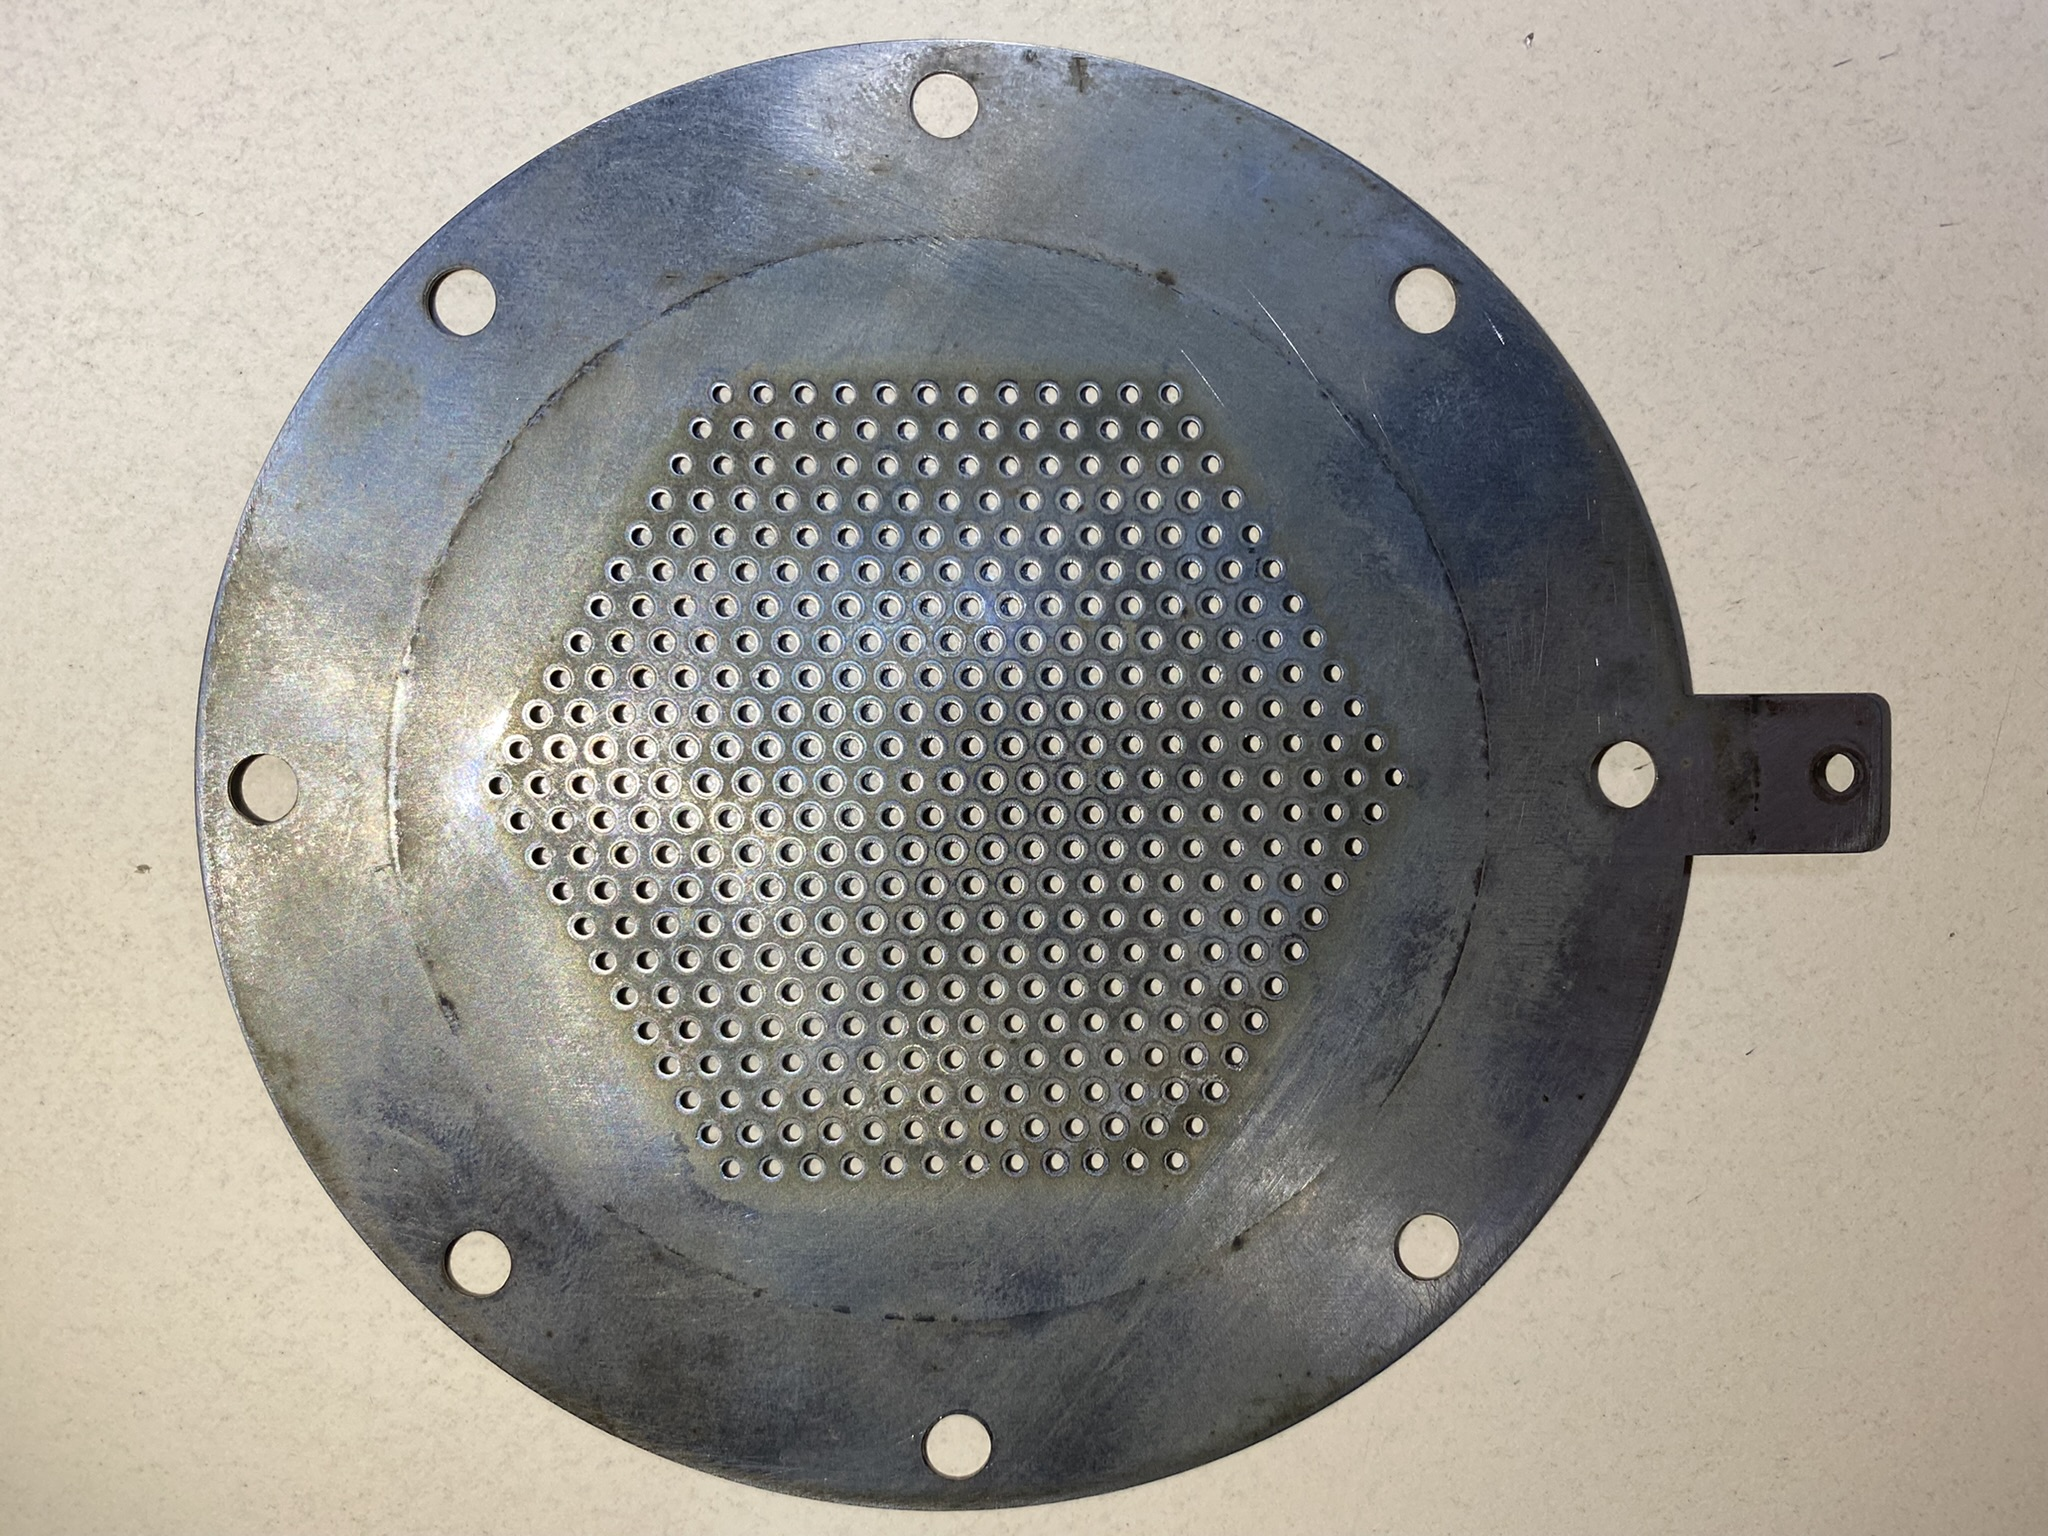
\includegraphics[scale=0.15]{fig/accel.jpeg}
    \caption{Accelerator grid of BURFIT-80}
    \label{fig:burfitaccel}
\end{figure}

When oppositely biased, grids create an electrostatic field and exploit the plasma sheath that forms at the intersection of plasma and grid surfaces.
 Accelerator grid is negatively biased in order to attract positively charged ions in the plasma. When directly exposed to plasma high speed collisions between ions and accelerator grid cause sputtering and erode the grid, effectively reducing its lifetime. In order to shield the accelerator grid and properly channel the ion flow, screen grid is used. When located in between the accelerator grid and biased positively, screen grid forces ions to channel through the grids. Potential variations of grids is shown in graph at figure \ref{fig:potvariation}.
 Biasing voltages for screen grid and accel grid are in the range of +200V and -1000V respectively. 
\newpage
 \begin{figure}[ht]
     \centering
     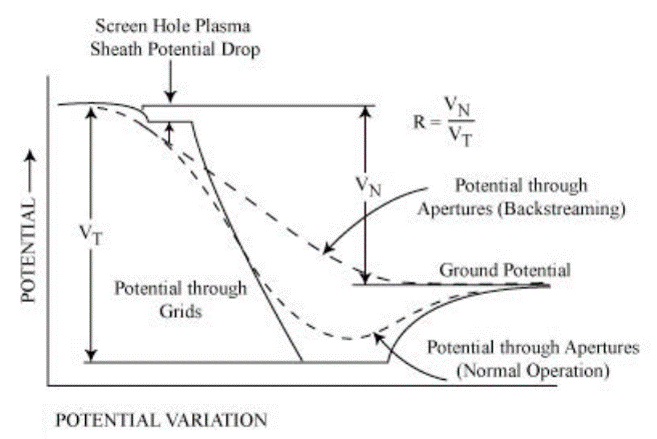
\includegraphics[scale=0.9]{fig/potvariation.png}
     \caption[Grid Potential Variations]{Grid Potential Variations\cite{OCW1964}}
     \label{fig:potvariation}
 \end{figure}
  
 In order to ensure robust channeling of ions through the grids the screen and accelerator grids need to be properly aligned and distanced. Diameters of apertures in grids are also determined accordingly. Diameter of screen grid apertures are generally larger than that of accelerator grid apertures. When grids are properly aligned and ion flow is optimal then grid structure reaches its optimum perveance levels as shown in figure \ref{fig:ionflow}

\begin{figure}[ht]
    \centering
    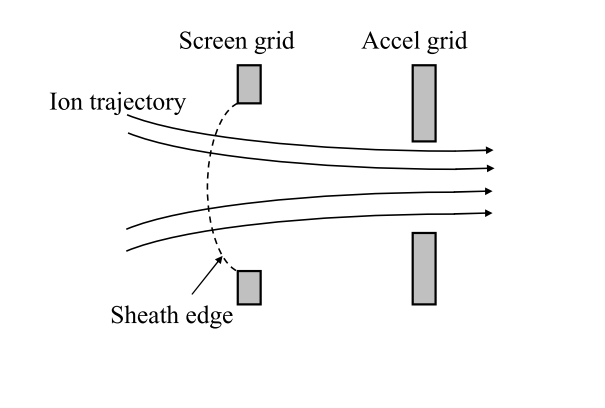
\includegraphics[scale=0.6]{fig/ionflow.png}
    \caption[Ion flow through screen and accelerator grids]{Ion flow through screen and accelerator grids\cite{williams2013ion}}
    \label{fig:ionflow}
\end{figure}

In the event of grid misalignment ion trajectory may display undesirable behaviours such as under-perveance or over-perveance. 
\begin{figure}[ht]
    \centering
    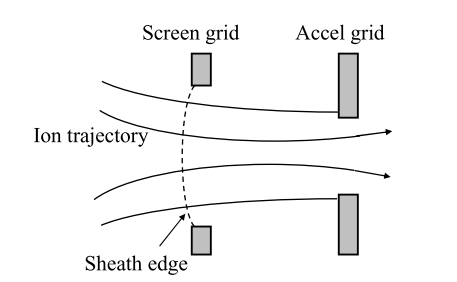
\includegraphics[scale=0.6]{fig/overperveance.png}
    \caption[Over-perveance trajectory of ions]{Overperveance trajectory of ions\cite{williams2013ion}}
    \label{fig:overperveance}
\end{figure}

Figure \ref{fig:overperveance} displays a situation called overperveance in which over focusing ions cause increased ion sputtering on the grids.

\begin{figure}[ht]
    \centering
    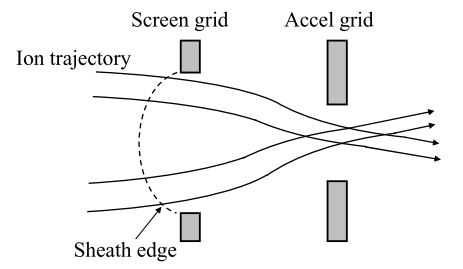
\includegraphics[scale=0.6]{fig/underperveance.png}
    \caption[Under-perveance trajectory of ions]{Overperveance trajectory of ions\cite{williams2013ion}}
    \label{fig:underperveance}
\end{figure}


Another misalignment type occurs when the ions are insufficiently focused in which case ions display a motion shown in figure \ref{fig:underperveance}. This behavior is referred as under-perveance. 

Proper ion flow is dominated by grid aperture and distance parameters shown in figure \ref{fig:gridparams}.
\newpage
\begin{figure}[ht]
    \centering
    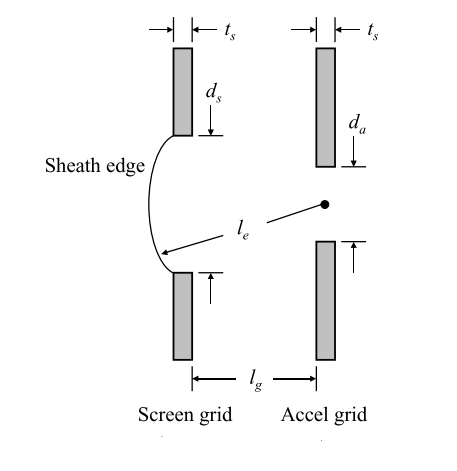
\includegraphics[scale=0.6]{fig/gridparameters.png}
    \caption[Grid structure parameters]{Grid structure parameters\cite{williams2013ion}}
    \label{fig:gridparams}
\end{figure}

In figure \ref{fig:ionflow} $d_s$ and $d_a$ are screen grid aperture and accelerator grid aperture diameter respectively. $l_g$ is the distance between grids. $t_s$ and $t_a$ are thickness of screen and accelerator grid, respectively. Finally, $l_e$ is the effective ion acceleration distance. 

Upon exiting the thrusters ions form beamlets which occur at the downstream direction of grid apertures. Afterwards beamlets mix together and form one continuous ion beam. However occasionally positively charged accelerated ions may backstream towards similarly positively biased accelerator. Ion beamlets, forming of ion beam and backstreaming ions are illustrated in figure \ref{fig:ionbackstream}.

\begin{figure}[ht]
    \centering
    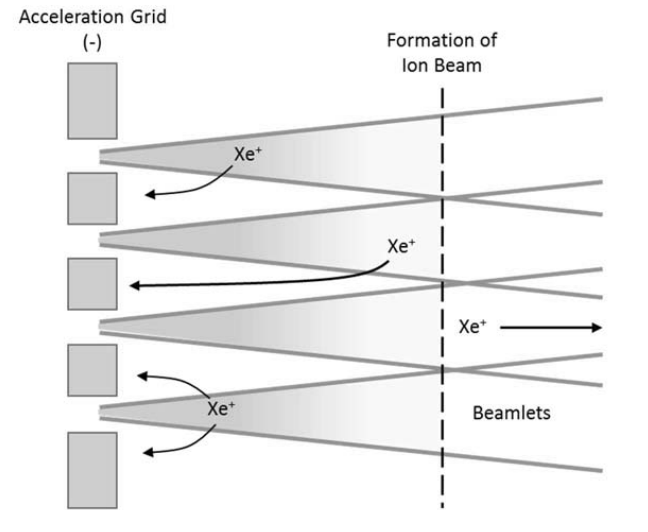
\includegraphics[scale=0.6]{fig/ionbackstream.png}
    \caption[Ion beamlets, beam and escaping ions]{Ion beamlets, beam and escaping ions\cite{Couch2017}}
    \label{fig:ionbackstream}
\end{figure}
Over time collisions between backstreaming ions and accelerator grid can cause erosion significantly reduce the grid's ability to channel ions properly. In order to avoid damage to accelerator grid an additional grid, named \textit{decelerator} grid, can be placed in the downstream direction of ion beam. Decelerator grid is kept at ground potential and shields the accelerator grid from high energy impacts. Placement and working principle of decelerator grid is shown in figure \ref{fig:ionbackstreamdecel}

\begin{figure}[ht]
    \centering
    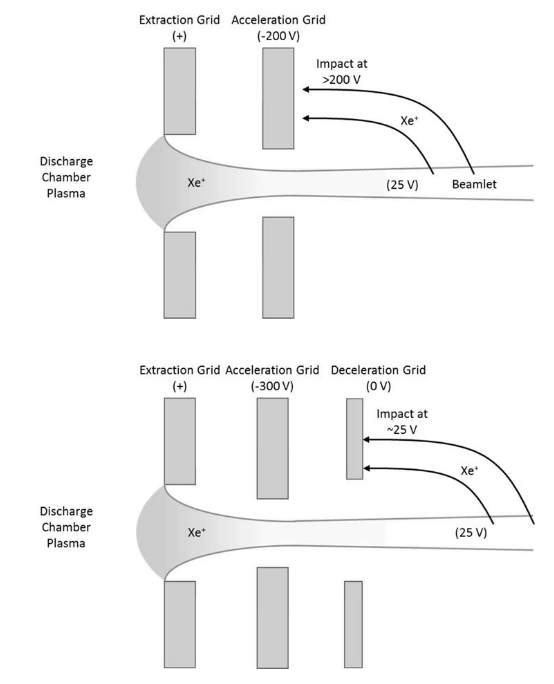
\includegraphics[scale=0.75]{fig/ionbackstreamdecel.png}
    \caption[Comparison of Two and Three Grid Designs]{Comparison of Two and Three Grid Designs\cite{Couch2017}}
    \label{fig:ionbackstreamdecel}
\end{figure}

Electric field vector between grids is in the direction of ion flow; from screen to accelerator grid as shown in figure \ref{fig:gridpot}. 

\begin{figure}[ht]
    \centering
    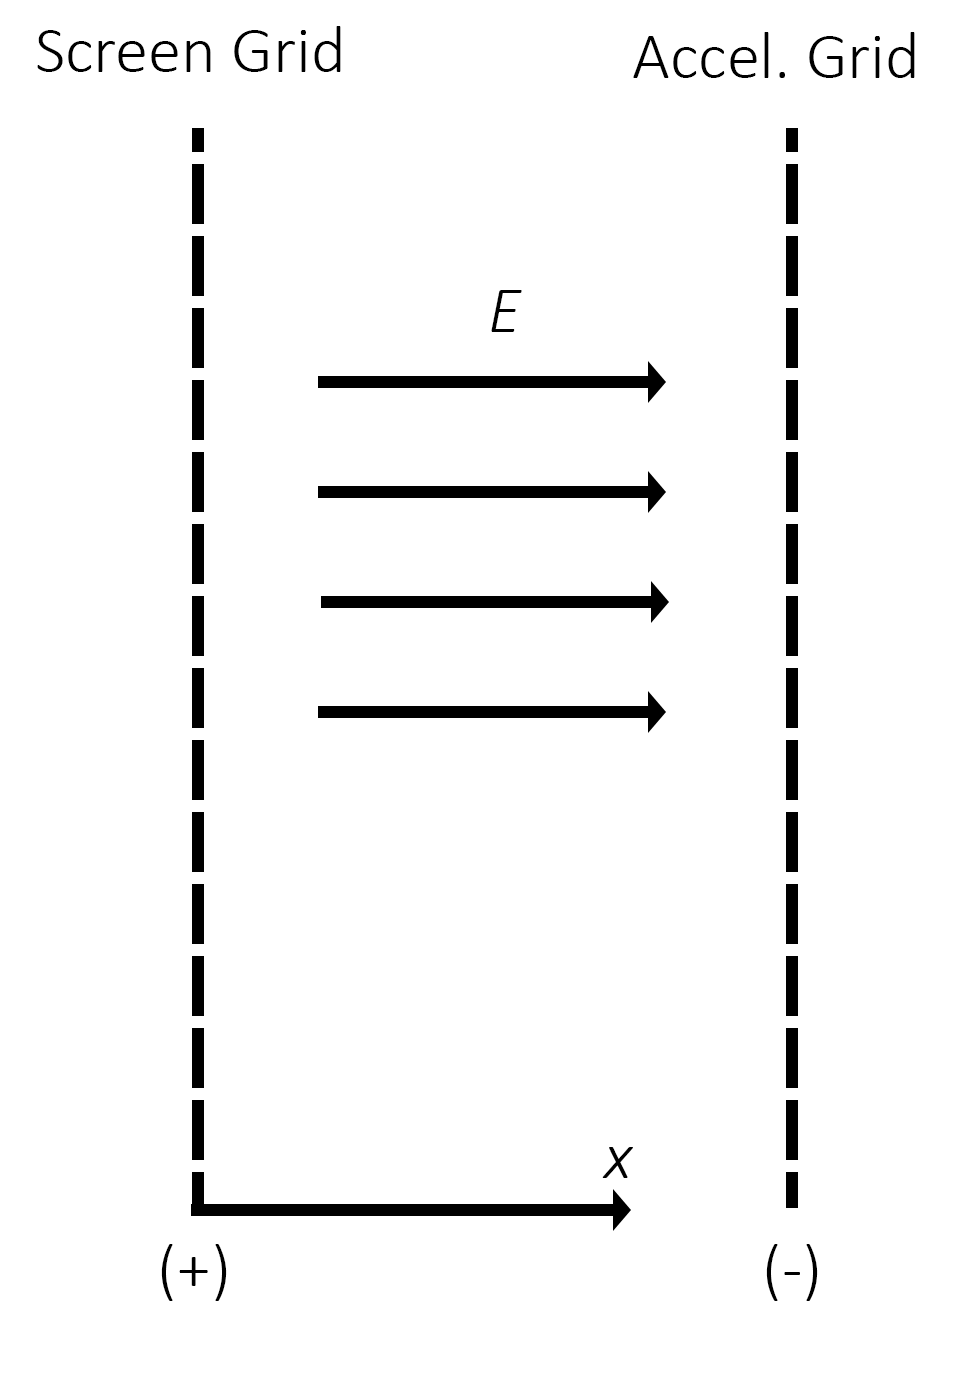
\includegraphics[scale=0.3]{fig/gridpot.png}
    \caption{Electric field vector between grids}
    \label{fig:gridpot}
\end{figure}
\newpage

Within the gap in between grids, Poisson's equation holds\cite{OCW1964};

\begin{equation}
    \frac{d^2\phi}{dx^2} = -\frac{e n_i}{\varepsilon_0}
    \label{eq:poisson}
\end{equation}

where $e$ is the electric charge and $n_i$ is the number of ions. Together, $e n_i$ constitutes $\rho$, charge density. Ion continuity between grids is constant;

\begin{equation}
    j = e n_i v_i
    \label{eq:ioncont}
\end{equation}

where $v_i$ is ion velocity due to electrostatic free-fall.

Particles in the gap is subjected to force $F=qE$.
\begin{equation}
   F =  qE = -e \frac{d \phi}{dx} = m_i \frac{dv}{dt}
    \label{eq:gapforce}
\end{equation}

Multiplying all sides with $dx$ gives;

\begin{equation}
    -ed\phi = m_i\frac{dx}{dt}dv = m_i v dv
    \label{eq:dv}
\end{equation}

\begin{eqnarray}
    ed\phi + m_i v dv = 0
    \label{eq:eq0}
\end{eqnarray}

Taking the integral of \ref{eq:eq0};

\begin{equation}
    e\phi + \frac{1}{2}m_i v^2_i = e\phi_0 + \frac{1}{2}m_i v^2_0
    \label{eq:integrated}
\end{equation}

\begin{equation}
    v^2_i - v^2_0 = \frac{2e(\phi_0 - \phi)}{m_i}
\end{equation}

Assuming inital speeds of ions are negligible;

\begin{equation}
    v_i = \sqrt{\frac{2e(\phi_0 - \phi)}{m_i}}
    \label{eq:ionvel}
\end{equation}


Plugging equations \ref{eq:ioncont} and \ref{eq:ionvel} into equation \ref{eq:poisson} gives 2nd order nonlinear differential equation for electic field between gaps where the potential $\phi$ is known;

\begin{equation}
    \frac{d^2 \phi}{d x^2} + \frac{j}{\varepsilon_0}\sqrt{\frac{m_i}{2e (\phi_0-\phi)}} = 0
    \label{eq:2ndorder}
\end{equation}

Rearranging and integrating equation \ref{eq:2ndorder} gives $E$;

\begin{equation}
    E^2 = \left(\frac{d\phi}{dx}\right)^2 - \left(\frac{d\phi}{dx}\right)^2_{x=0}  = \frac{4j}{\varepsilon_0}\sqrt{\frac{m_i (\phi_0 -\phi)}{2e}}
    \label{eq:integratedE}
\end{equation}

where boundary conditions are\cite{OCW1964};

\begin{equation}
    \begin{aligned}
        \phi(0) = 0 \\
        \phi(x=d) = -V_T
    \end{aligned}
    \label{eq:boundary1}
\end{equation}

where $d$ is the distance between grids and $V_T$ is the accel. grid potential. 

Furthermore another fundamental boundary condition imposed\cite{OCW1964};

\begin{equation}
    \left(\frac{d\phi}{dx}\right)_{x=0}
    \label{eq:boundary2}
\end{equation}

Which can be imposed due to "space charge limitation". When there is no ion flow electric field between grids is constant and dependent on the potentials of screen and accel. grids. As the ions flow from screen to accel. grid electric field is altered. There comes a point where accelerating field near the first grid is cancelled by the downstream of positively charged ions. At this point the grids are accelerating highest current density possible and is space charge limited\cite{lara2016design}. 

\begin{equation}
    E = \frac{d\phi}{dx} \left(\frac{4j}{\varepsilon_0}\right)^{\frac{1}{2}}\left(\frac{m_i (\phi_0 - \phi)}{2e}\right)^{\frac{1}{2}}
\end{equation}

Integrating;

\begin{equation}
    \phi_{x=d} - \phi_{x=0} = - \left[\frac{3}{2}\left(\frac{j}{\varepsilon_0}\right)^{\frac{1}{2}}\left(\frac{m_i}{2e}\right)^{\frac{1}{4}}x\right]^{\frac{4}{3}}\bigg| ^{x=d}_{x=0}
\end{equation}

Substituting boundary conditions from equations \ref{eq:boundary1} and \ref{eq:boundary2} and rearranging gives;

\begin{equation}
    J = \frac{4}{9}\varepsilon_0 \sqrt{\frac{2e}{m_i}}\frac{V_T^{\frac{3}{2}}}{d^2}
    \label{eq:childlangmuir}
\end{equation}

Equation \ref{eq:childlangmuir} gives maximum current density extracted from polarized grids and is referred as Child-Langmuir's Law in which J is current per unit area, $m_i$ is mass of ions, $V_T$ is voltage and $d$ is the sheath thickness.. In order to Relation of Child-Langmuir's Law and thrust calculations will be examined in subsection \ref{ch:subsecthrust}.

Grid structure is constantly in contact with plasma and ions throughout the lifetime of the thruster and thus subjected to heating. In order to preserve grid alignment, grid materials should be chosen from materials with low heat expension coefficient. Additionally chosen material should also exhibit low secondary electron yield\cite{Bumbarger}. In practice grids are generally manufactured from molybdenum, titanium, INVAR or even carbon composite materials\cite{yavuz2013prototype}.
% \subsection{RF Coil}
\subsection{Thrust} \label{ch:subsecthrust}
Thrust is created by accelerating positively charged ions to high velocities and ejecting them from the thruster. Momentum transfer between ions and thruster occurs within accelerator grids thus thrust can be defined by sum of forces applied on screen and accelerator grids\cite{Couch2017} as shown in equations \ref{eq:gridforce} and \ref{eq:gridforcesum}.

\begin{equation}
    \begin{aligned}
        F_{screen} = \frac{1}{2}\epsilon_0 E^2_{screen} \\
        F_{accel} = -\frac{1}{2}\epsilon_0 E^2_{accel} 
    \end{aligned}
\label{eq:gridforce}
\end{equation}

\begin{equation}
    F = F_{screen} + F_{accel} = \frac{1}{2}\epsilon_0 (E^2_{screen}-E^2_{accel})
    \label{eq:gridforcesum}
\end{equation}

Thrust calculations can also be performed by evaluating the momentum change with respect to time;

\begin{equation}
T = \frac{d}{dt}(mv) = \frac{d}{dt}(m_p v_{ex}) =  \dot{m}_p v_{ex}    
\label{eq:momentumchange}
\end{equation}

where $\dot{m}_p$ is the propellant flow rate and $v_{ex}$ is the exhaust velocity. Equation \ref{eq:momentumchange} is same for all thruster systems. Specifically for electric propulsion systems it can be refined as;

\begin{equation}
    T = \dot{m}_p v_{ex} \sim \dot{m}_i v_i
    \label{eq:epthrust}
\end{equation}

Since ion thrusters achieve most of its thrust from ejected ions, propellant mass and exhaust velocity in equation \ref{eq:momentumchange} can be exchanged with ion mass flow rate 
$\dot{m}_i$ and ion velocity $v_i$\cite{goebel2008fundamentals}.

Electric energy is converted into kinetic energy in the thruster.

\begin{equation}
    \frac{1}{2}m_i v_i = e V_b
    \label{eq:kineticenergy}
\end{equation}

Where $V_b$ is the ion beam potential. From equation \ref{eq:kineticenergy} ion velocity $v_i$ can be defined as;

\begin{equation}
    v_i = \sqrt{\frac{2eV_b}{m_i}}
    \label{eq:ionvel2}
\end{equation}

Ion beam current, $I_b$, for fully and singly ionized propellant is defined as\cite{goebel2008fundamentals};

\begin{equation}
    I_b = \dot{m}_i\left(\frac{e}{m_i}\right)
    \label{eq:ionbeamcurrent}
\end{equation}

Substituting equations \ref{eq:ionvel2} and \ref{eq:ionbeamcurrent} into equation \ref{eq:epthrust} gives the thrust formula;

\begin{equation}
    T = \sqrt{\frac{2 m_i V_b}{e}} I_b
    \label{eq:uncorrectedthrust}
\end{equation}

Thrust defined in equation \ref{eq:uncorrectedthrust} is applicable for ideal conditions only. Unideal conditions during thruster operations warrant the inclusion  of additional correction factors. 

One of the unideal conditions is ion beam divergence. Ions contribute to thrust only when they are moving in the opposite direction of spacecraft velocity vector. Other ions diverting from this direction do not provide thrust and are considered as loss. 

\begin{figure}[ht]
    \centering
    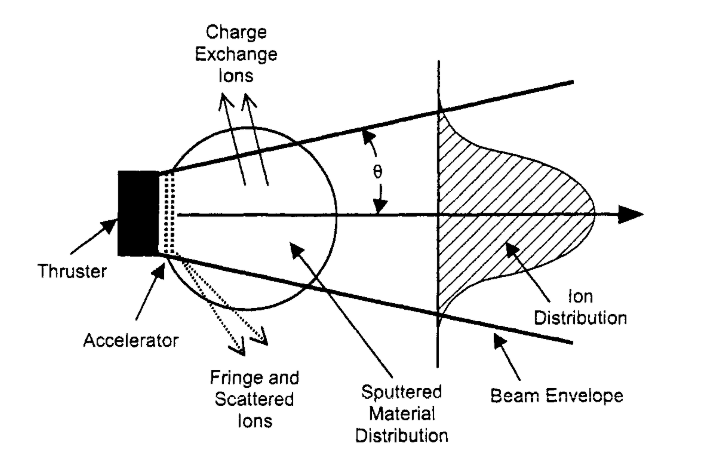
\includegraphics[scale=.75]{fig/beamdivergence.png}
    \caption[Beam plume behaviour after exiting thruster]{Beam plume behaviour after exiting thruster\cite{goebel2008fundamentals}}
    \label{fig:beamdivergence}
\end{figure}

In the figure \ref{fig:beamdivergence}, angle $\theta$ is defined as half-angle of ion beam divergence. It can also be observed in figure \ref{fig:beamdivergence2} which was taken during when BURFIT-80 thruster was operating. 

\begin{figure}[ht]
    \centering
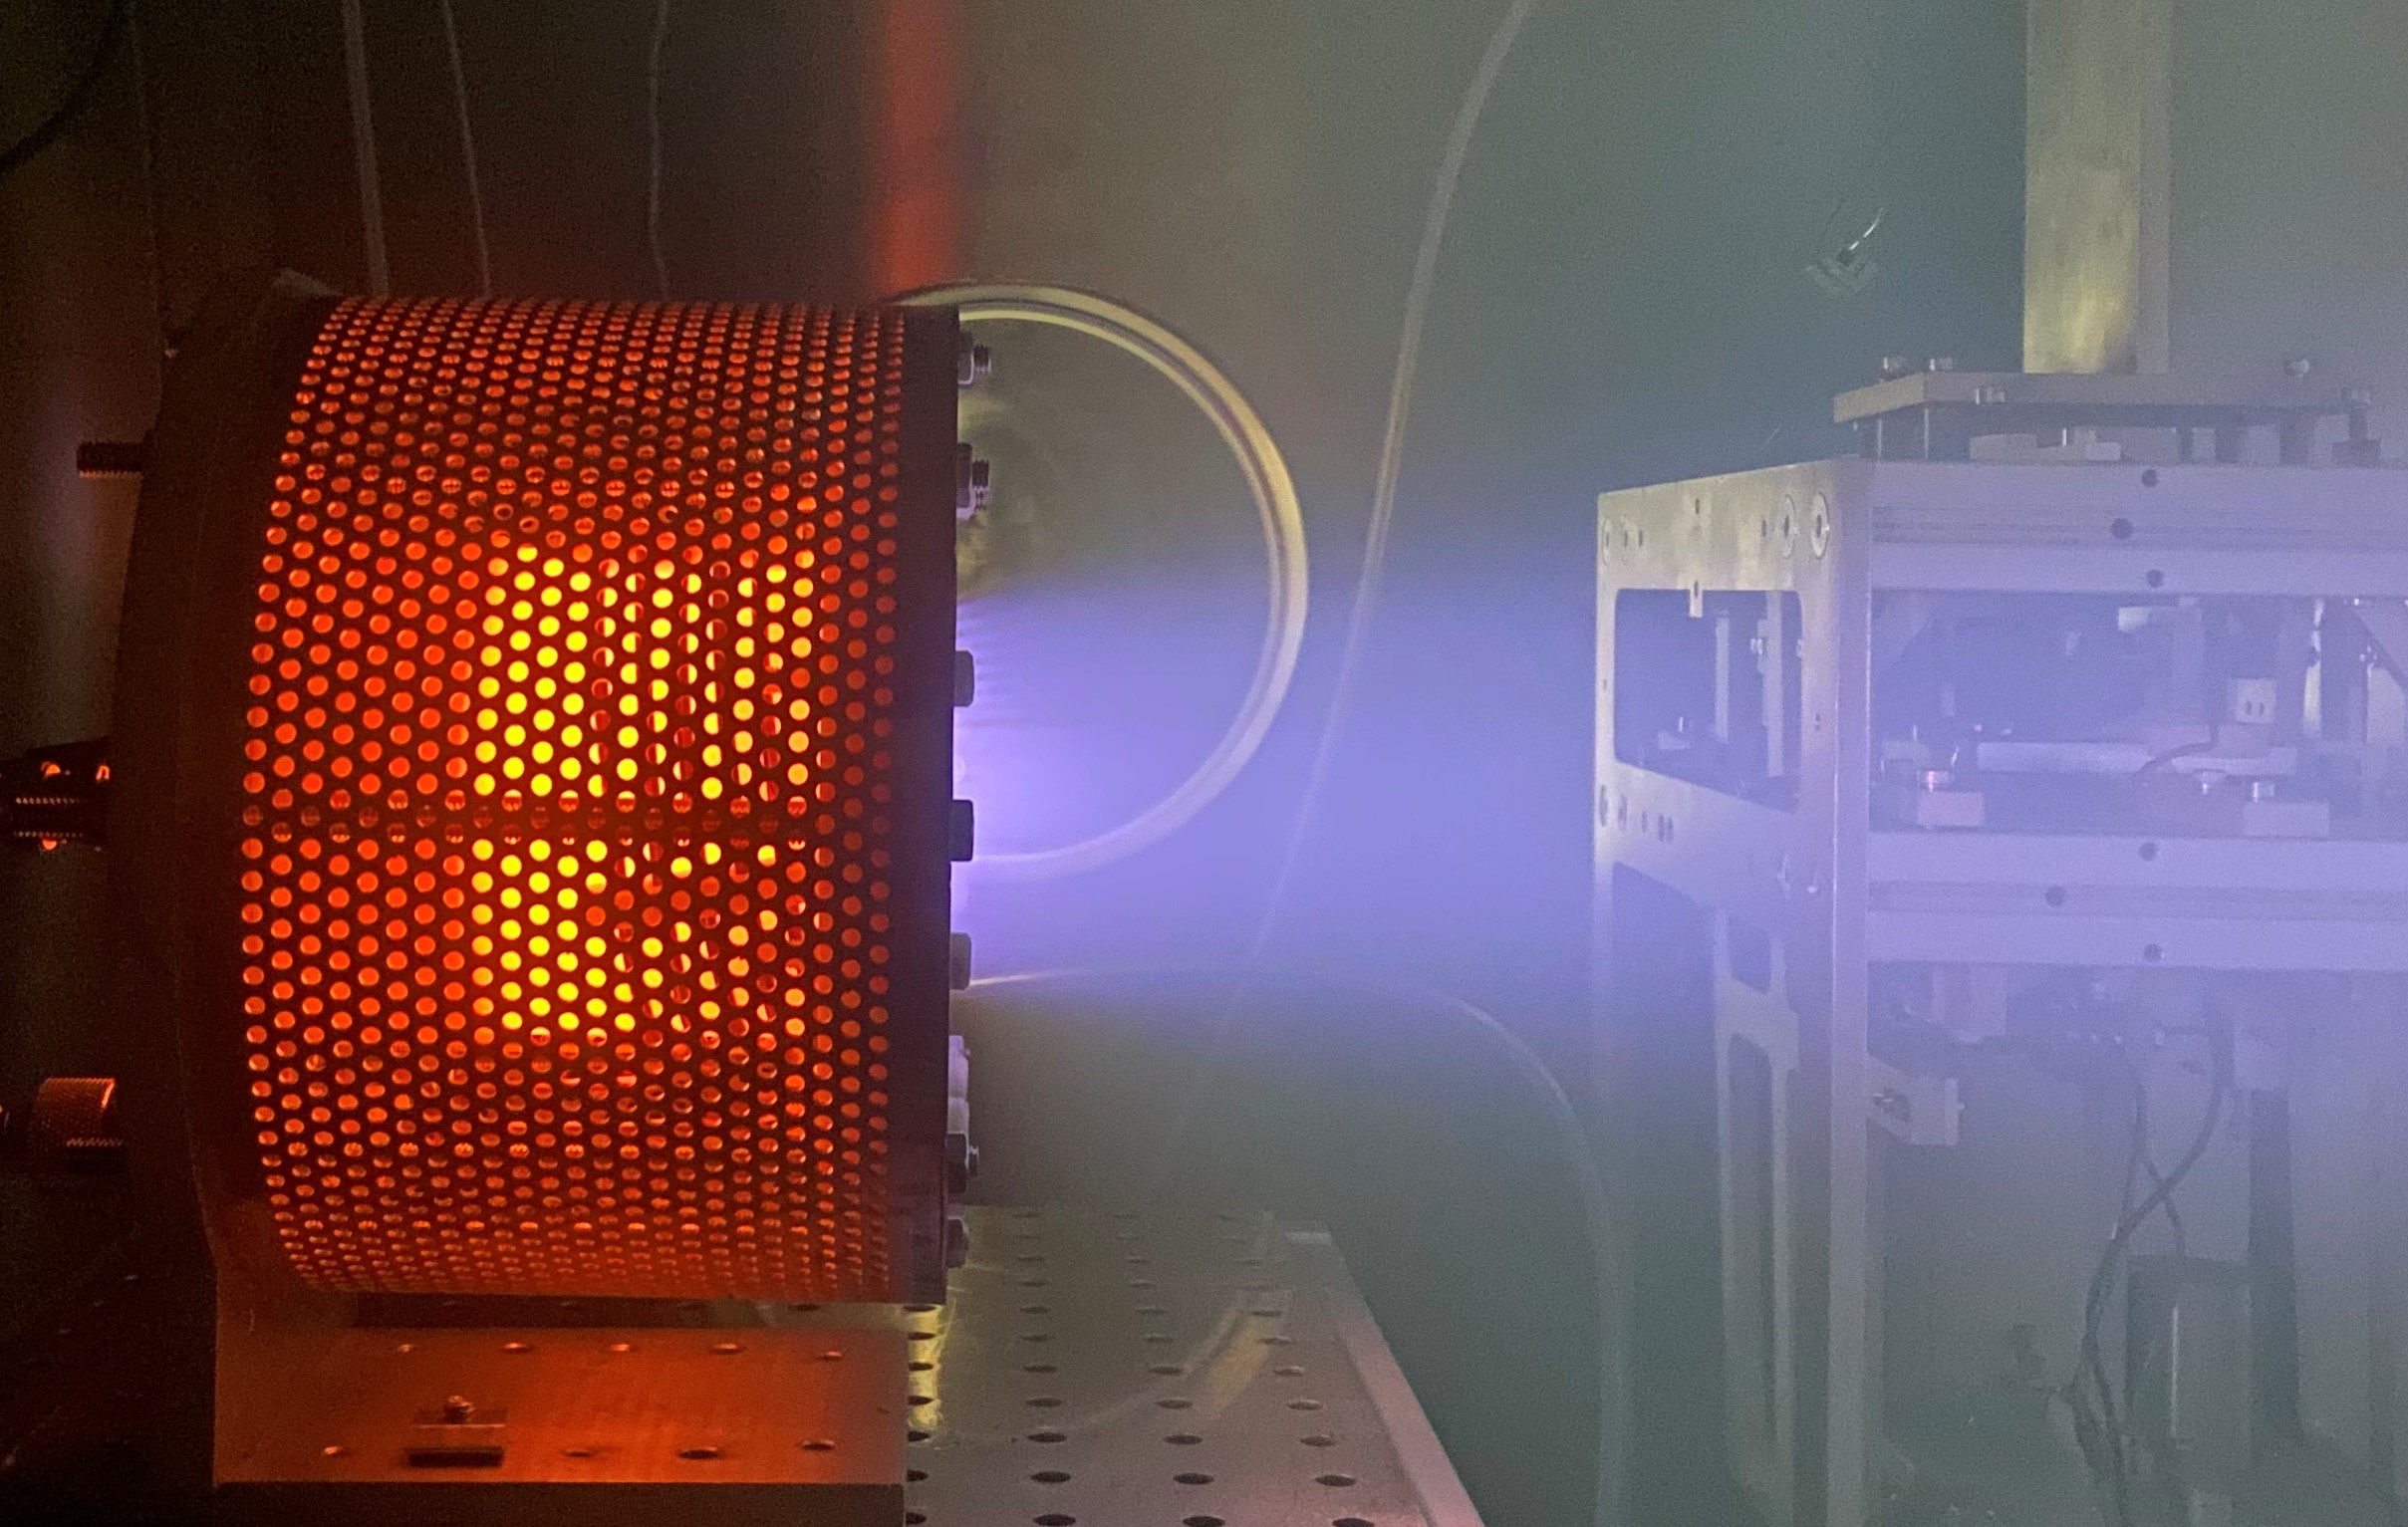
\includegraphics[scale=0.15]{fig/beamdiv.jpg}
\caption{Ion beam and divergence of BURFIT-80}
\label{fig:beamdivergence2}
\end{figure}

In figure \ref{fig:beamdivergence2} it can be clearly seen that beam originating from the thruster is dispersing in a direction perpendicular to the thruster axis. In order to include a correction factor for thrust calculations following formula is introduced. 

\begin{equation}
    F_t = cos\theta
    \label{eq:divergenceangle}
\end{equation}

Second factor to consider in thrust calculations is the ratio of doubly charged ions to singly charged ions. Electron with a sufficient energy can collide with an already ionized particle
and can release a second electron, creating a doubly ionized particle. Doubly ionized particles require more energy to ionize and consume the kinetic energy which could be otherwise be used to singly-ionize other particles. In order to account for this energy loss coefficient $\alpha$ is introduced. It is defined as\cite{goebel2008fundamentals};

\begin{equation}
    \alpha = \frac{I^+ + \dfrac{1}{\sqrt{2}I^{++}}}{I^+ + I^{++}} =  \frac{1+0.707\dfrac{I^{++}}{I+}}{1+\dfrac{I^{++}}{I^+}}
    \label{eq:alpha}
\end{equation}

where $I^+$ and $I^{++}$ are singly charged ion and doubly charged ion current respectively. Combining both correction factors from equations \ref{eq:divergenceangle} and \ref{eq:alpha} gives thrust correction coefficient $\gamma$;

\begin{equation}
    \gamma = \alpha F_t 
    \label{eq:gamma}
\end{equation}

Subsequently thrust formula from equation \ref{eq:uncorrectedthrust} turns into;

\begin{equation}
    T = \gamma \sqrt{\dfrac{2m_i V_b}{e}}I_b
    \label{eq:correctedthrust}
\end{equation}

Equation \ref{eq:correctedthrust} will be used to calculate thrust levels of designed prototype in chapter \ref{ch:Ch3}.

\subsection{Specific Impulse}
As mentioned earlier in chapter \ref{purposeofthesis} specific impulse is a measure to assess the thrusters propellant usage efficiency. It is defined as\cite{goebel2008fundamentals};
\begin{equation}
    I_{sp} = \frac{T}{\dot{m}_p g}
    \label{eq:specimpulse}
\end{equation}

Substituting the T expression from equation \ref{eq:momentumchange} gives;

\begin{equation}
    I_{sp} = \frac{v_{ex}}{g}
    \label{eq:specimpulse2}
\end{equation}

Substituting equation \ref{eq:epthrust} for $v_{ex}$ gives;

\begin{equation}
    I_{sp} = \frac{v_i}{g}\frac{\dot{m}_i}{\dot{m}_p}
    \label{eq:specimpulse3}
\end{equation}

in which the part $\dfrac{\dot{m}_i}{\dot{m}_p}$, ratio of ionized propellant to non-ionized propellant is defined as mass utilization efficiency $\eta_m$.

\begin{equation}
    I_{sp} = \frac{v_i}{g}\eta_m
    \label{eq:specimpulse4}
\end{equation}

Using equation \ref{eq:ionvel2} for ion velocity and adding correction factor $\gamma$ to account for correction factors as in thrust calculations gives;

\begin{equation}
    I_{sp} = \frac{\eta_m}{g}\sqrt{\frac{2e V_b}{I_b}}
    \label{eq:specimpulse5}
\end{equation}

Equation \ref{eq:specimpulse5} will be used to calculate specific impulse values in chapter \ref{ch:Ch3}.

% \subsection{RF System Design}
% \subsection{Power Consumption}
% \subsection{Efficiency}
\subsection{Neutralizer}
As the thruster fires positively charged ions will rapidly leave the thruster which will cause the spacecraft to be negatively charged. This situation is undesirable since loss of spacecraft's electrical ground will inevitably cause other subsystems of the spacecraft to stop properly functioning. Also positively charged particles in the ion beam can backstream into the thruster itself or adhere themselves to other sensitive surfaces of the spacecraft.  In order to compensate for this imbalanced load a neutralizer is placed in such position that emitted electrons will neutralize the ion beam. This neutralizer can be a complex system such as hollow cathode, shown in figure \ref{fig:burfitneut} or can be simple such as a tungten filament, shown in figure \ref{fig:tungstenneut}. 

\begin{figure}[ht]
    \centering
    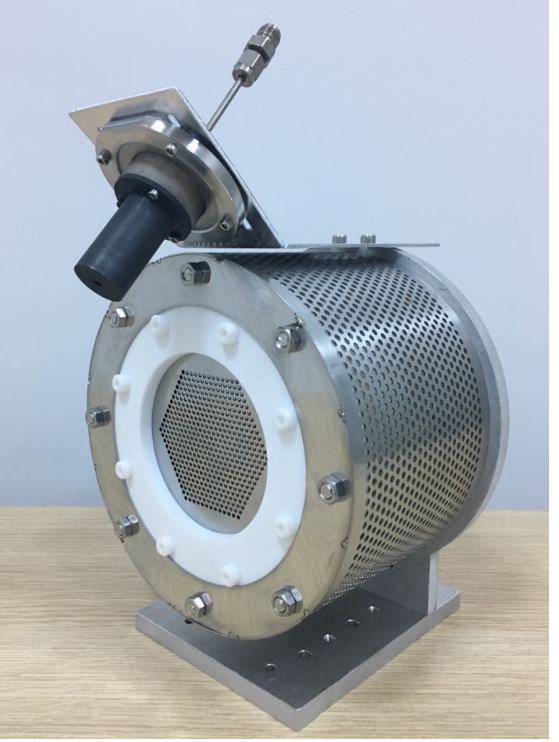
\includegraphics[scale=0.5]{fig/burfitneut.png}
    \caption[BURFIT-80 with neutralizer hollow cathode attached on top]{BURFIT-80 with neutralizer hollow cathode attached on top\cite{kokal2019development}}
    \label{fig:burfitneut}  
\end{figure}

\begin{figure}[ht]
    \centering
    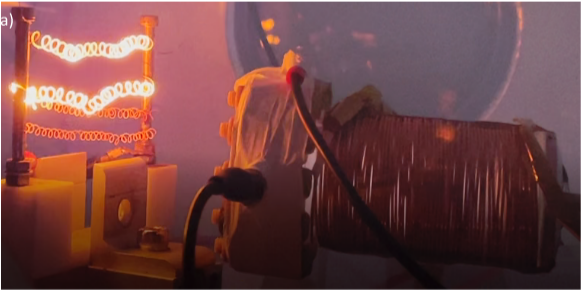
\includegraphics[scale=0.75]{fig/tungstenneut.png}
    \caption{Thruster operation with tungsten filament placed at ion beam downstream(\textbf{ATIF YAYINLANMADI})}
    \label{fig:tungstenneut}  
\end{figure}

Although a neutralizer is essential for space operations, in this work it is not included. This is because testing is conducted in a vacuum chamber that has its wall grounded, effectively
negating the need for an external neutralizer. 

% Tables and figures given in appendices must be numbered with the number of the appendix they are in (i.e. Table \ref{TableA.1}, Table A.2, Figure A.1, Figure A.2).

% In tables and figures, font size could be reduced to 8 pt, if necessary.

% Tables must be prepared using the same font type as the thesis. The font type used in figures must be consistent throughout the thesis.

% Tables and figures must be placed after they are first cited in the main text body, but must be as close as possible, in accordance with the rules in this guideline (Figure \ref{Figure2.1}). All tables and figures must be cited before they are used in the main text body (Table \ref{Table2.1}).

% All tables and figures must be horizontally centered on the page.

% The numbering of the tables and the figures must be such that the first number is the number of the chapter the table/figure is placed under (for appendices, the letter of the appendix), and the second number is the number of order (i.e. Table \ref{Table2.2}, Figure \ref{Figure2.2}, Table \ref{TableA.1}, Figure \ref{Figure2.3}). The words “Table” and “Figure” and numbers must be bold.

% For table numbers and captions, 1 line spacing, 12 pt (before) and 6 pt (after) paragraph spacing must be set. Table captions must be ended with a full stop. A table and its caption must be on the same page. 

% Multiple tables/figures could be placed on one page, however, table/figures spanning more than 4 consecutive pages must be given in appendices rather than the main text body.

% The first paragraph following a table must have 12 pt (before) and 6 pt (after) paragraph spacing. Titles following a table must have the standard formatting as previously specified. 

% Footnotes for a table must be written with 1 line spacing and a font size 2 pt smaller than the main text body. 
% For figure numbers and captions, 1 line spacing, 6 pt (before) and 12 pt (after) paragraph spacing must be set. Figure captions must be ended with a full stop. A figure and its caption must be on the same page. 

% For figures spanning more than one page, the same number and caption must be written below the continued figure, with the expression ”continued” added in brackets (i.e. \textbf{Table \ref{Table2.1} (continued):} Metal composition of wastes. \textbf{Figure \ref{Figure2.1} (continued):} Water supply network of ISTANBUL.).

% Plots, images and musical notes must be numbered and captioned as figures. Musical notes must be written according to the format rules set by the ITU School of Traditional Turkish Music. 

% It is recommended that elements that increase the page thickness and disrupt the binding structure of theses such as  folded pages or additional items embedded on pages are given as appendices.

% \vspace{6pt}
% \begin{figure}[h]
% 	\centering
% 	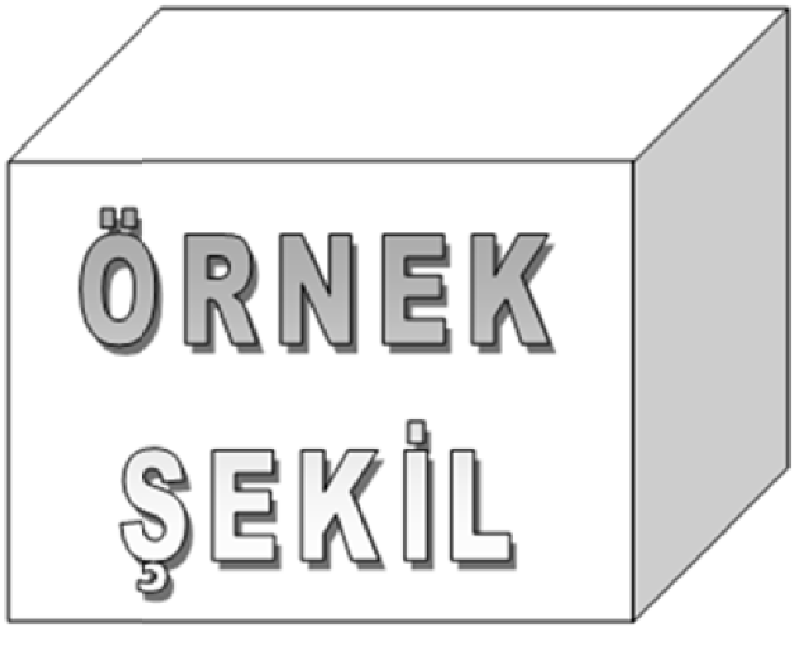
\includegraphics[scale=.3]{./fig/sekil1}
% 	% sekil1.eps: 0x0 pixel, 300dpi, 0.00x0.00 cm, bb=14 14 592 479
% 	\vspace{6pt}
% 	\caption{All tables and figures must be horizontally centered on the page.}
% 	\label{Figure2.1}
% \end{figure}

%\begin{figure}
%	\begin{minipage}[b]{.5\linewidth}
%		\centering
%		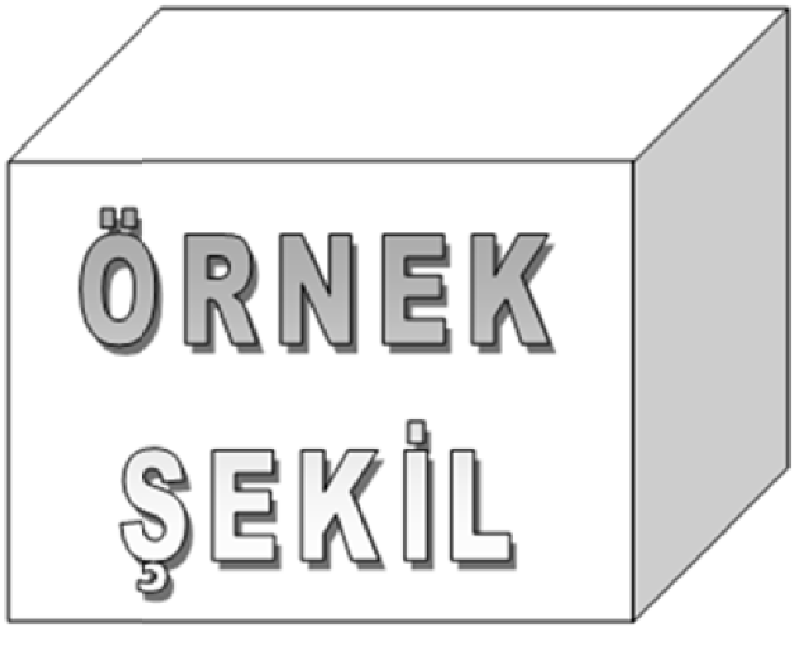
\includegraphics[scale=.2]{./fig/sekil1}
%		\subcaption{A subfigure}\label{Figure2.2a}
%	\end{minipage}
%	\begin{minipage}[b]{.5\linewidth}
%		\centering
%		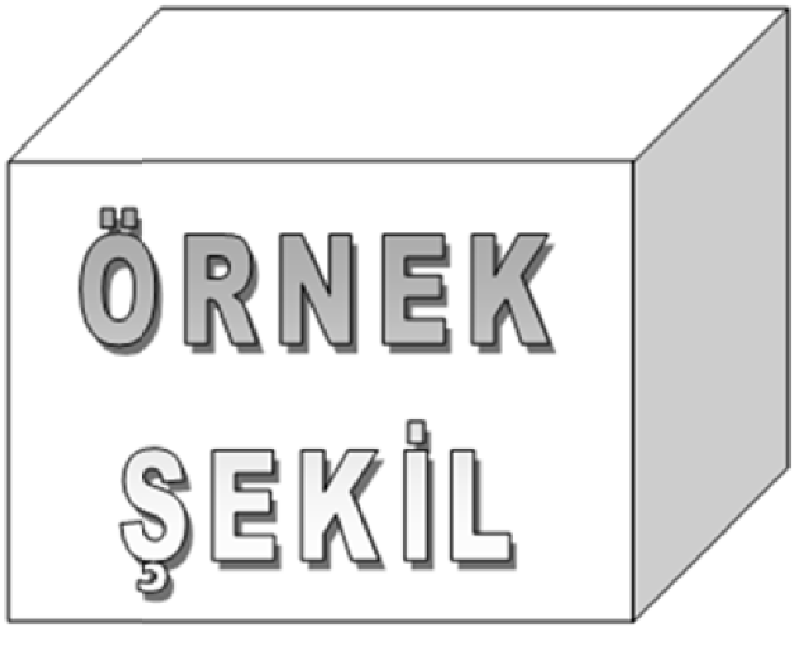
\includegraphics[scale=.2]{./fig/sekil1}
%		\subcaption{Another subfigure}\label{Figure2.2b}
%	\end{minipage}
%	\caption{A figure}\label{Figure2.2} % If no need a caption for main figure comment it out 
%\end{figure}
%%Figure letter: \subref{Figure2.2a}

%\begin{figure}
%	\begin{subfigure}[b]{.5\linewidth}
%		\centering
%		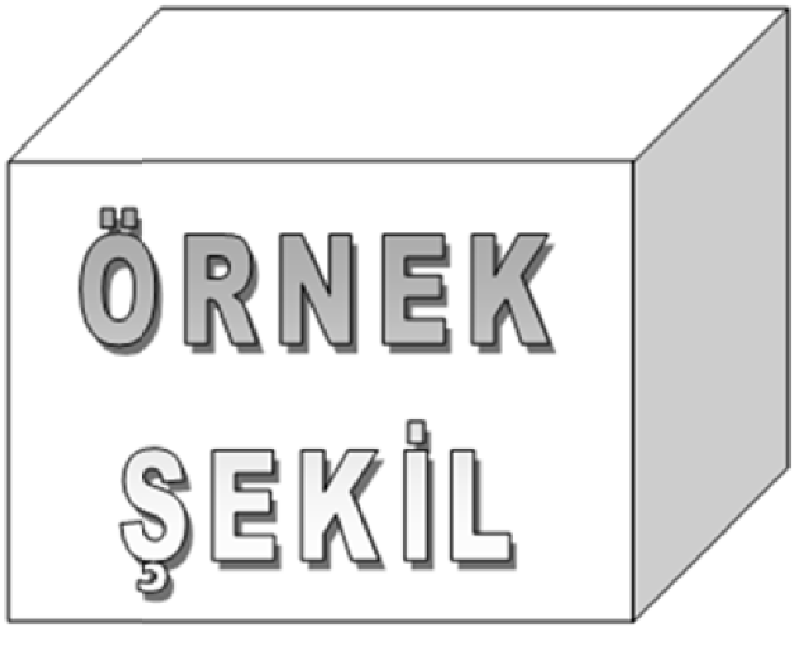
\includegraphics[scale=.2]{./fig/sekil1}
%		\caption{A subfigure}\label{Figure2.3a}
%	\end{subfigure}
%	\begin{subfigure}[b]{.5\linewidth}
%		\centering
%		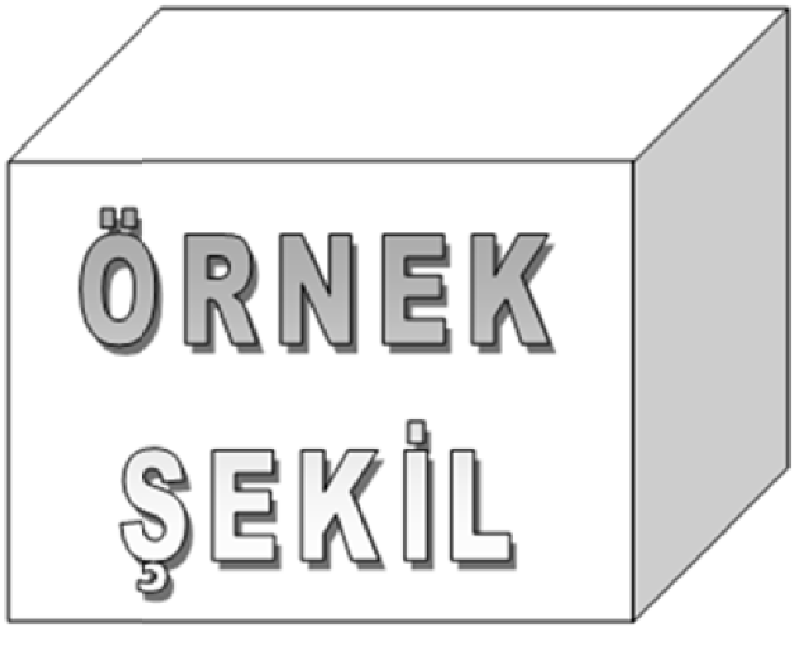
\includegraphics[scale=.2]{./fig/sekil1}
%		\caption{Another subfigure}\label{Figure2.3b}
%	\end{subfigure}
%	\caption{A figure}\label{Figure2.3}
%\end{figure}

% Subfigure example with proper LOF usage - SBÖ
% \begin{figure}[h]
% 	\centering
% 	\begin{subfigure}{.8\textwidth}
% 		\centering
% 		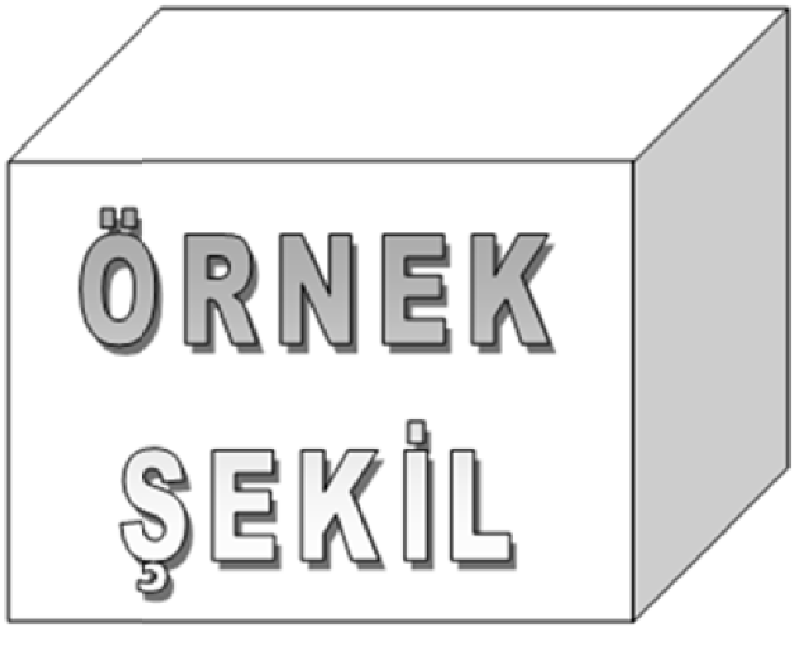
\includegraphics[scale=.3]{./fig/sekil1}
% 		\firstsubcaption{First subcaption of the subfigure.}
% 		\label{Figure2.2a}
% 	\end{subfigure}
% 	\begin{subfigure}{.8\textwidth}
% 		\centering
% 		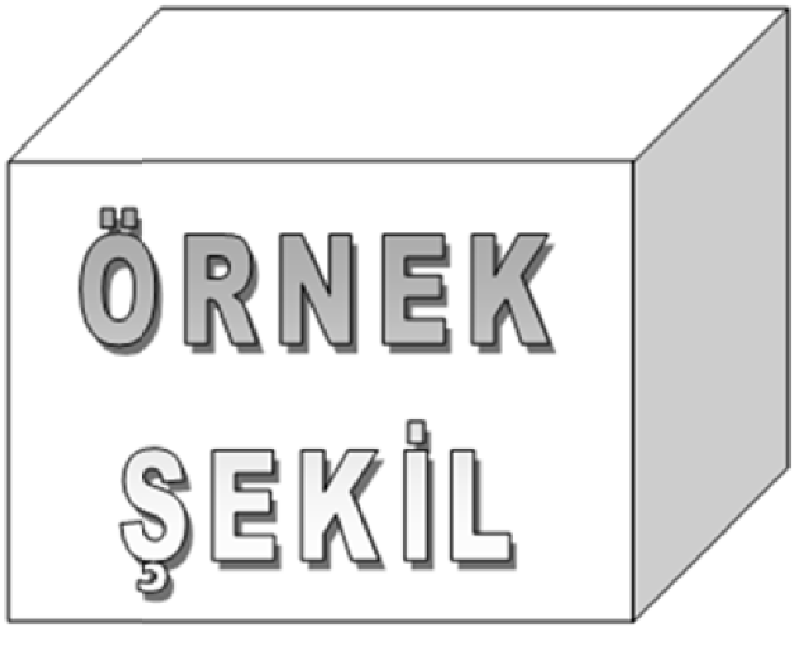
\includegraphics[scale=.3]{./fig/sekil1}
% 		\nextsubcaption{Second subcaption of the subfigure.}
% 		\label{Figure2.2b}
% 	\end{subfigure}
%     \caption{An example of subfigure main caption.}\label{Figure2.2}
% \end{figure}

%\begin{figure}
%	\centering     % not \center
%	\subcaption[]{Another subfigure}{\label{fig:a}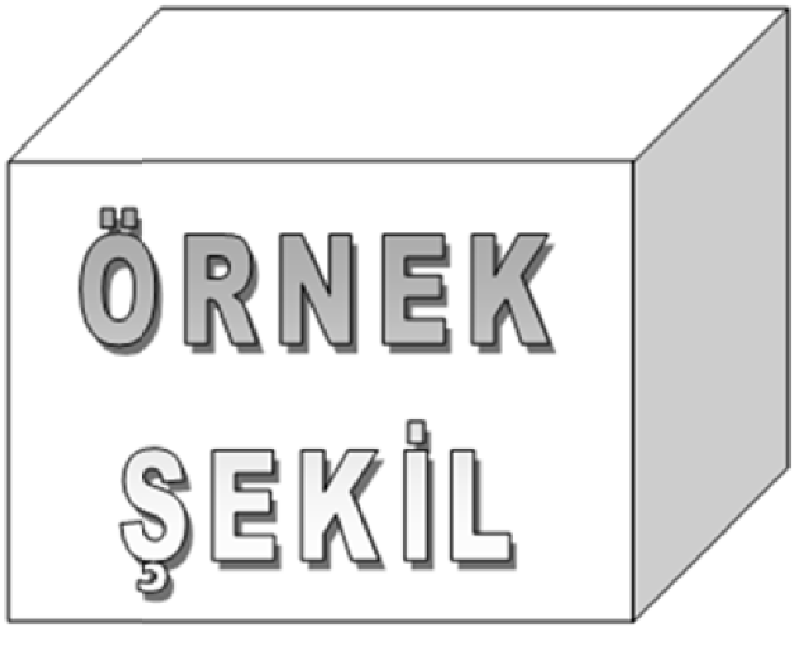
\includegraphics[scale=.2]{./fig/sekil1}}
%	\subcaption[]{Another subfigure}{\label{fig:b}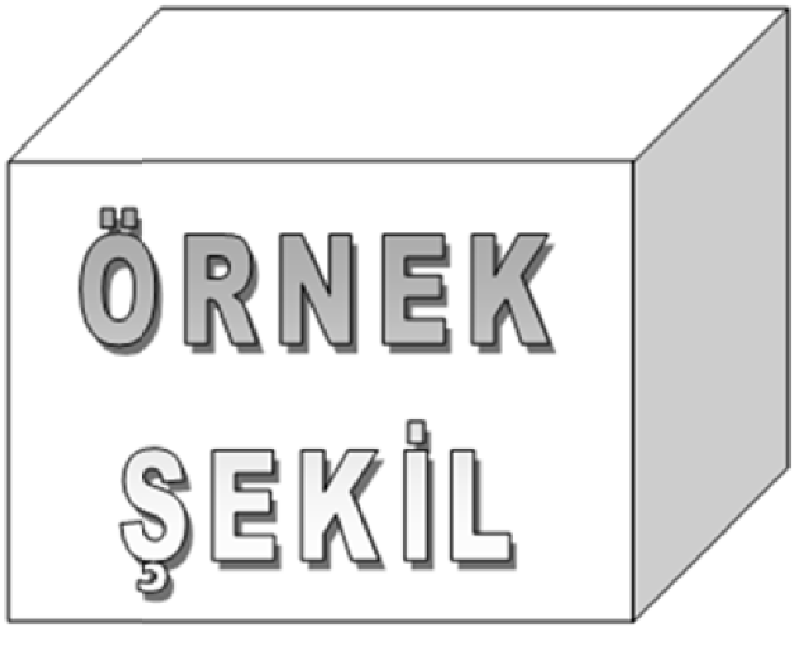
\includegraphics[scale=.2]{./fig/sekil1}}
%	%\caption{(a) this is fig 1 (b) this is fig 2.}
%	\label{L50}
%\end{figure}

% In Figure \ref{Figure2.2}, sed diam nonumy eirmod tempor invidunt ut labore et dolore magna aliquyam erat, sed diam voluptua. At vero eos et accusam et justo duo dolores et ea rebum. Lorem ipsum dolor sit amet, consetetur sadipscing elitr, sed diam nonumy eirmod tempor invidunt ut labore et dolore magna aliquyam erat, sed diam voluptua. At vero eos et accusam et justo duo dolores et ea rebum. At vero eos et accusam et justo duo dolores et ea rebum. At vero eos et accusam et justo duo dolores et ea rebum. At vero eos et accusam et justo duo dolores et ea rebum. At vero eos et accusam et justo duo dolores et ea rebum. At vero eos et accusam et justo duo dolores et ea rebum. At vero eos et accusam et justo duo dolores et ea rebum in Figure \ref{Figure2.2a}.

% \begin{figure}
% 	\centering
% 	
\includegraphics[width=10cm,keepaspectratio=true]{./fig/sekil2}
% 	% sekil2.eps: 0x0 pixel, 300dpi, 0.00x0.00 cm, bb=14 14 818 556
% 	\vspace{3pt}
% 	\caption{Example figure.}
% 	\label{Figure2.3}
% \end{figure}
% \vspace{-6pt}
% \section{Landscape-oriented, full-page figure}


% % Change margins on the fly to reset the page margins to one inch - SBÖ
% \newenvironment{changemargin}[4]{
% 	\begin{list}{}{
% 			\setlength{\voffset}{#1}
% 			\setlength{\oddsidemargin}{#2}
% 			\setlength{\evensidemargin}{#3}
% 			\setlength{\textheight}{#3}
% 		}
% 		\item[] ~ \par
% 		% Get rid of the extra space inserted by the previous line
% 		%\vspace*{-2em}
% 	}{
% 	\end{list}
% }

% % All the figures and also odd page figures normally face inside the thesis, however the rule requires figures always face to the right. - SBÖ
% % Figures on landscape pages has to be centered and facing to the right (ITU) - SBÖ
% \begin{landscape}
% 	\thispagestyle{empty} %Remove the bottom page numbering
% %	\begin{changemargin}{-0.4mm}{0mm}{0mm} %Set all the margins to zero - SBÖ
% 	%\thispagestyle{lscape}
% 	\vspace*{5mm}
% 	\begin{figure*}[ht]
% 		\centering
% 		%\begin{tabular}{@{}cc@{}}
% 		
\includegraphics[scale=.41,keepaspectratio=true]{./fig/sekil3} %&
% 		%
\includegraphics[width=50mm]{./fig/sekil3}
% 		%\end{tabular}                                       
% 		\caption{Landscape-oriented, full-page figure.}
% 		\label{Figure2.4}
% 	\end{figure*}
	
% % Set the page number on the right side for odd numbered pages
%       \begin{tikzpicture}[remember picture, overlay]
% 		\node[xshift=-25mm+148.5mm, yshift=17mm-210mm+15mm] (number) at (current page text area.east) {\thepage};
% 	  \end{tikzpicture}
	  
% %\end{changemargin}
% \end{landscape}

% % All the figures and also even page figures normally face inside the thesis, however the rule requires figures always face to the right. - SBÖ
% % Figures on landscape pages has to be centered and facing to the right (ITU) - SBÖ
% \begin{landscape}
% 	\thispagestyle{empty} % Remove the bottom page numbering
% %	\begin{changemargin}{-0.4mm}{0mm}{0mm} %Set all the margins to zero - SBÖ
% 		%\thispagestyle{lscape}

% 		\vspace*{20mm}
% 		\begin{figure*}[ht]
% 			\centering
% 			%\begin{tabular}{@{}cc@{}}
% 				
\includegraphics[scale=.41,keepaspectratio=true]{./fig/sekil3} %&
% 				%
\includegraphics[width=50mm]{./fig/sekil3}
% 			%\end{tabular}                                       
% 			\caption{Landscape-oriented, full-page figure.}
% 			\label{Figure2.5}
% 		\end{figure*}
	   
% % Set the page number on the left side for even numbered pages
% 		%\begin{tikzpicture}[remember picture, overlay]
% 		% \node[xshift=-25mm+148.5mm, yshift=-1mm-15mm, rotate=180] (number) at (current page text area.east) {\thepage};
% 		%\end{tikzpicture}
		
% % Set the page number on the right side for even numbered pages as well
% 		\begin{tikzpicture}[remember picture, overlay]
% 		 \node[xshift=-25mm+148.5mm, yshift=17mm-210mm] (number) at (current page text area.east) {\thepage};
% 		\end{tikzpicture}
		
% %	\end{changemargin}
% \end{landscape}

% %\newpage
% \section{Table Citations and Table Example}
% \begin{table*}[h]
% 	{\setlength{\tabcolsep}{14pt}
% 		\caption{Table with single row and centered columns.}
% 		\begin{center}
% 			\vspace{-6mm}
% 			\begin{tabular}{cccc}
% 				\hline \\[-2.45ex] \hline \\[-2.1ex]
% 				Column A & Column B & Column C & Column D \\
% 				\hline \\[-1.8ex]
% 				Row A & Row A & Row A & Row A \\
% 				Row B & Row B & Row B & Row B \\
% 				Row C & Row C & Row C & Row C \\
% 				\hline
% 			\end{tabular}
% 			\vspace{-6mm}
% 		\end{center}
% 		\label{Table2.1}}
% \end{table*}

% As seen in Table \ref{Table2.1}, 
% \begin{table*}[h]
% 	{\setlength{\tabcolsep}{14pt}
% 		\caption{Table captions must be ended with a full stop.}
% 		\begin{center}
% 			\vspace{-6mm}
% 			\begin{tabular}{cccc}
% 				\hline \\[-2.45ex] \hline \\[-2.1ex]
% 				Column A & Column B & Column C & Column D \\
% 				\hline \\[-1.8ex]
% 				Row A & Row A & Row A & Row A \\
% 				Row B & Row B & Row B & Row B \\
% 				Row C & Row C & Row C & Row C \\
% 				\hline
% 			\end{tabular}
% 			\vspace{-6mm}
% 		\end{center}
% 		\label{Table2.2}}
% \end{table*}



% \section{Landscape-oriented, full-page table}


% % ---------------------------------------------------------------- %
% % Page numbers must be on the bottom-middle of short side (when    %
% % portrait-oriented), or bottom-middle of long side (when	       %
% % landscape-oriented)						                       %
% % ---------------------------------------------------------------- %
% % Odd page landscape table and page numbering - SBÖ		
% \begin{landscape}
% 	\thispagestyle{empty}
% %	\vspace*{-6mm}
% %	\begin{changemargin}{0.4mm}{0mm}{0mm} %Set all the margins to zero - SBÖ
% 	\begin{table*}[htb!]
% 		{\setlength{\tabcolsep}{14pt}
% 			%\hspace*{5mm}
% 			%\vspace*{-6mm}
% 			\caption{Prof. Dr. Galip TEPEHAN \,\, Captioning in landscape-oriented pages:
% 				the most important aspect is to align the lines horizontally.}
% 			\begin{center}
% 				\vspace{-6mm}
% 				\begin{tabular}{lccrrrrr}
% 					\hline\hline
% 					\multirow{2}{*}{Parametre} & \multirow{2}{*}{Column 2} & \multirow{2}{*}{Column 3} & \multicolumn{3}{c|}{Column 4} & \multicolumn{2}{c}{Column 5}\\ \cline{4-8}
% 					& & & Subcolumn & Subcolumn & Subcolumn & Subcolumn & Subcolumn\\
% 					\hline
% 					Row 1 & -7.680442 & 7.6986348 & 0.00 & 0.00 & 0.00 & 12 & 12 \\
% 					Row 2 & 140 & - & 0.50 & 0.00 & 0.00 & 0 & 0 \\
% 					Row 3 & 37.174357 & 37.16192697 & 0.00 & 0.00 & 0.00 & 0 & 24 \\
% 					Row 4 & 140 & - & 0.50 & 0.00 & 0.00 & 0 & 0 \\
% 					Row 5 & 37.174357 & 37.16192697 & 0.00 & 0.00 & 0.00 & 0 & 24 \\
% 					Row 6 & 140 & - & 0.50 & 0.00 & 0.00 & 0 & 0 \\
% 					Row 7 & 37.174357 & 37.16192697 & 0.00 & 0.00 & 0.00 & 0 & 24 \\
% 					Row 8 & 140 & - & 0.50 & 0.00 & 0.00 & 0 & 0 \\
% 					Row 9 & 37.174357 & 37.16192697 & 0.00 & 0.00 & 0.00 & 0 & 24 \\
% 					Row 10 & 140 & - & 0.50 & 0.00 & 0.00 & 0 & 0 \\
% 					Row 11 & 37.174357 & 37.16192697 & 0.00 & 0.00 & 0.00 & 0 & 24 \\
% 					Row 12 & 140 & - & 0.50 & 0.00 & 0.00 & 0 & 0 \\
% 					Row 13 & 37.174357 & 37.16192697 & 0.00 & 0.00 & 0.00 & 0 & 24 \\
% 					Row 14 & 140 & - & 0.50 & 0.00 & 0.00 & 0 & 0 \\
% 					Row 15 & 37.174357 & 37.16192697 & 0.00 & 0.00 & 0.00 & 0 & 24 \\
% 					\hline
% 				\end{tabular}
% 			\end{center}
% 			\begin{center}
% 				\label{Table2.3}
% 			\end{center}
% 		}
% 	\end{table*}
% % Set the page number on the right side for odd numbered pages
% 		\begin{tikzpicture}[remember picture,overlay]
% 		\node[xshift=-10mm+148.5mm, yshift=2mm-210mm+30mm] (number) at (current page text area.east) {\thepage};
% 		\end{tikzpicture}
% %   \end{changemargin}
% \end{landscape}

% % ---------------------------------------------------------------- %
% % Page numbers must be on the bottom-middle of short side (when    %
% % portrait-oriented), or bottom-middle of long side (when	       %
% % landscape-oriented)						                       %
% % ---------------------------------------------------------------- %
% % Even page landscape table and page numbering - SBÖ		
% \begin{landscape}
% 	\thispagestyle{empty}
% 	%\vspace*{-6mm}
% %	\begin{changemargin}{0.4mm}{0mm}{0mm} %Set all the margins to zero - SBÖ
% 		\begin{table*}[htb!]
% 			{\setlength{\tabcolsep}{14pt}
% 				%\hspace*{5mm}
% 				%\vspace*{-6mm}
% 				\caption{Prof. Dr. Galip TEPEHAN \,\, Captioning in landscape-oriented pages:
% 					the most important aspect is to align the lines horizontally.}
% 				\begin{center}
% 					\vspace{-6mm}
% 					\begin{tabular}{lccrrrrr}
% 						\hline\hline
% 						\multirow{2}{*}{Parametre} & \multirow{2}{*}{Column 2} & \multirow{2}{*}{Column 3} & \multicolumn{3}{c|}{Column 4} & \multicolumn{2}{c}{Column 5}\\ \cline{4-8}
% 						& & & Subcolumn & Subcolumn & Subcolumn & Subcolumn & Subcolumn\\
% 						\hline
% 						Row 1 & -7.680442 & 7.6986348 & 0.00 & 0.00 & 0.00 & 12 & 12 \\
% 						Row 2 & 140 & - & 0.50 & 0.00 & 0.00 & 0 & 0 \\
% 						Row 3 & 37.174357 & 37.16192697 & 0.00 & 0.00 & 0.00 & 0 & 24 \\
% 						Row 4 & 140 & - & 0.50 & 0.00 & 0.00 & 0 & 0 \\
% 						Row 5 & 37.174357 & 37.16192697 & 0.00 & 0.00 & 0.00 & 0 & 24 \\
% 						Row 6 & 140 & - & 0.50 & 0.00 & 0.00 & 0 & 0 \\
% 						Row 7 & 37.174357 & 37.16192697 & 0.00 & 0.00 & 0.00 & 0 & 24 \\
% 						Row 8 & 140 & - & 0.50 & 0.00 & 0.00 & 0 & 0 \\
% 					\end{tabular}
% 				\end{center}
% 				\begin{center}
% 					\label{Table2.4}
% 				\end{center}
% 			}
% 		\end{table*}
% % Set the page number on the right side for even numbered pages
% 		\begin{tikzpicture}[remember picture,overlay]
% 		\node[xshift=-25mm+148.5mm, yshift=2mm-210mm+15mm] (number) at (current page text area.east) {\thepage};
% 		\end{tikzpicture}
% %	\end{changemargin}
% \end{landscape}

% \begin{table}[!htbp] \centering
% 	\caption{ Neighborhoods Visited }
% 	\vspace{-3mm}
% 	\label{}
% 	\begin{tabular}{@{\extracolsep{5pt}} llrrr} 
% 	\\[-1.8ex]\hline 
% 		\hline \\[-1.8ex] 
% 		\multicolumn{1}{c}{Variable} & \multicolumn{1}{c}{Values} & \multicolumn{1}{c}{Count} & \multicolumn{1}{c}{\%} & \multicolumn{1}{c}{Cum. \%} \\
% 		\hline \\[-1.8ex] 
% 		\multirow{ 4 }{*}{ visit }  &  FALSE  &  2  &  33.33  &  33.33  \\
% 		\hhline{}  &  TRUE  &  3  &  50.00  &  83.33  \\
% 		\hhline{}  &  NA  &  1  &  16.67  &  100.00  \\
% 	    \hhline{}  &  Total  &  6  &  100.00  &    \\
% 		\hline \\[-1.8ex] 
% 	\end{tabular}
% \end{table}

% % Multi-page longtable example spreading couple of pages - SBÖ
% \begin{center}
% 	\begin{longtable}{ccc}
% 		%Here is the caption, the stuff in [] is the table of contents entry,
% 		%the stuff in {} is the title that will appear on the first page of the
% 		%table.
% 		\caption[Feasible triples for a highly variable Grid]{Feasible triples
% 			for highly variable Grid, MLMMH.} \label{Table2.6} \vspace{-1.75mm}\\
% 		%This is the header for the first page of the table...
% 		\hline\\[-2.45ex] \hline \\[-1.8ex] % Distancing of the hlines adjausted from the text 
% 		\multicolumn{1}{c}{{Time (s)}} &
% 		\multicolumn{1}{c}{{Triple chosen}} &
% 		\multicolumn{1}{c}{{Other feasible triples}} \\[0.5ex] \hline
% 		\\[-1.8ex]
% 		\endfirsthead
		
% 		%This is the header for the remaining page(s) of the table...
% 		\multicolumn{3}{c}{{\tablename} \textbf{\thetable{}} \textbf{(continued) :} Feasible triples
% 			for highly variable Grid, MLMMH.} \\[0.5ex]
% 		\hline\\[-2.45ex] \hline \\[-1.8ex]
% 		\multicolumn{1}{c}{{Time (s)}} &
% 		\multicolumn{1}{c}{{Triple chosen}} &
% 		\multicolumn{1}{c}{{Other feasible triples}} \\[0.5ex] \hline
% 		\\[-1.8ex]
% 		\endhead
		
% 		%This is the footer for all pages except the last page of the table...
% 		%\multicolumn{3}{l}{{Continued on Next Page\ldots}} \\
% 		\\[-1.8ex] \hline
% 		\endfoot
		
% 		%This is the footer for the last page of the table...
% 		\\[-1.8ex] \hline
% 		\endlastfoot
		
% 		%Now the data...
% 		0      & (1, 11, 13725) & (1, 12, 10980), (1, 13, 8235), (2, 2, 0), (3, 1, 0) \\
% 		2745   & (1, 12, 10980) & (1, 13, 8235), (2, 2, 0), (2, 3, 0), (3, 1, 0) \\
% 		5490   & (1, 12, 13725) & (2, 2, 2745), (2, 3, 0), (3, 1, 0) \\
% 		8235   & (1, 12, 16470) & (1, 13, 13725), (2, 2, 2745), (2, 3, 0), (3, 1, 0) \\
% 		% <data removed>
% 		164700 & (1, 13, 13725) & (2, 2, 2745), (2, 3, 0), (3, 1, 0) \\
% 		0      & (1, 11, 13725) & (1, 12, 10980), (1, 13, 8235), (2, 2, 0), (3, 1, 0) \\
% 		2745   & (1, 12, 10980) & (1, 13, 8235), (2, 2, 0), (2, 3, 0), (3, 1, 0) \\
% 		5490   & (1, 12, 13725) & (2, 2, 2745), (2, 3, 0), (3, 1, 0) \\
% 		8235   & (1, 12, 16470) & (1, 13, 13725), (2, 2, 2745), (2, 3, 0), (3, 1, 0) \\
% 		% <data removed>
% 		164700 & (1, 13, 13725) & (2, 2, 2745), (2, 3, 0), (3, 1, 0) \\
% 		0      & (1, 11, 13725) & (1, 12, 10980), (1, 13, 8235), (2, 2, 0), (3, 1, 0) \\
% 		2745   & (1, 12, 10980) & (1, 13, 8235), (2, 2, 0), (2, 3, 0), (3, 1, 0) \\
% 		5490   & (1, 12, 13725) & (2, 2, 2745), (2, 3, 0), (3, 1, 0) \\
% 		8235   & (1, 12, 16470) & (1, 13, 13725), (2, 2, 2745), (2, 3, 0), (3, 1, 0) \\
% 		% <data removed>
% 		164700 & (1, 13, 13725) & (2, 2, 2745), (2, 3, 0), (3, 1, 0) \\
% 		0      & (1, 11, 13725) & (1, 12, 10980), (1, 13, 8235), (2, 2, 0), (3, 1, 0) \\
% 		2745   & (1, 12, 10980) & (1, 13, 8235), (2, 2, 0), (2, 3, 0), (3, 1, 0) \\
% 		5490   & (1, 12, 13725) & (2, 2, 2745), (2, 3, 0), (3, 1, 0) \\
% 		8235   & (1, 12, 16470) & (1, 13, 13725), (2, 2, 2745), (2, 3, 0), (3, 1, 0) \\
% 		% <data removed>
% 		164700 & (1, 13, 13725) & (2, 2, 2745), (2, 3, 0), (3, 1, 0) \\
% 		0      & (1, 11, 13725) & (1, 12, 10980), (1, 13, 8235), (2, 2, 0), (3, 1, 0) \\
% 		2745   & (1, 12, 10980) & (1, 13, 8235), (2, 2, 0), (2, 3, 0), (3, 1, 0) \\
% 		5490   & (1, 12, 13725) & (2, 2, 2745), (2, 3, 0), (3, 1, 0) \\
% 		8235   & (1, 12, 16470) & (1, 13, 13725), (2, 2, 2745), (2, 3, 0), (3, 1, 0) \\
% 		% <data removed>
% 		164700 & (1, 13, 13725) & (2, 2, 2745), (2, 3, 0), (3, 1, 0) \\
% 		0      & (1, 11, 13725) & (1, 12, 10980), (1, 13, 8235), (2, 2, 0), (3, 1, 0) \\
% 		2745   & (1, 12, 10980) & (1, 13, 8235), (2, 2, 0), (2, 3, 0), (3, 1, 0) \\
% 		5490   & (1, 12, 13725) & (2, 2, 2745), (2, 3, 0), (3, 1, 0) \\
% 		8235   & (1, 12, 16470) & (1, 13, 13725), (2, 2, 2745), (2, 3, 0), (3, 1, 0) \\
% 		% <data removed>
% 		164700 & (1, 13, 13725) & (2, 2, 2745), (2, 3, 0), (3, 1, 0) \\
% 		0      & (1, 11, 13725) & (1, 12, 10980), (1, 13, 8235), (2, 2, 0), (3, 1, 0) \\
% 		2745   & (1, 12, 10980) & (1, 13, 8235), (2, 2, 0), (2, 3, 0), (3, 1, 0) \\
% 		5490   & (1, 12, 13725) & (2, 2, 2745), (2, 3, 0), (3, 1, 0) \\
% 		8235   & (1, 12, 16470) & (1, 13, 13725), (2, 2, 2745), (2, 3, 0), (3, 1, 0) \\ \noalign{\penalty-5000}
% 		% <data removed>
% 		164700 & (1, 13, 13725) & (2, 2, 2745), (2, 3, 0), (3, 1, 0) \\
% 		0      & (1, 11, 13725) & (1, 12, 10980), (1, 13, 8235), (2, 2, 0), (3, 1, 0) \\
% 		2745   & (1, 12, 10980) & (1, 13, 8235), (2, 2, 0), (2, 3, 0), (3, 1, 0) \\
% 		5490   & (1, 12, 13725) & (2, 2, 2745), (2, 3, 0), (3, 1, 0) \\
% 		8235   & (1, 12, 16470) & (1, 13, 13725), (2, 2, 2745), (2, 3, 0), (3, 1, 0) \\
% 		% <data removed>
% 		164700 & (1, 13, 13725) & (2, 2, 2745), (2, 3, 0), (3, 1, 0) \\
% 		0      & (1, 11, 13725) & (1, 12, 10980), (1, 13, 8235), (2, 2, 0), (3, 1, 0) \\
% 		2745   & (1, 12, 10980) & (1, 13, 8235), (2, 2, 0), (2, 3, 0), (3, 1, 0) \\
% 		5490   & (1, 12, 13725) & (2, 2, 2745), (2, 3, 0), (3, 1, 0) \\
% 		8235   & (1, 12, 16470) & (1, 13, 13725), (2, 2, 2745), (2, 3, 0), (3, 1, 0) \\
% 		% <data removed>
% 		164700 & (1, 13, 13725) & (2, 2, 2745), (2, 3, 0), (3, 1, 0) \\
% 		0      & (1, 11, 13725) & (1, 12, 10980), (1, 13, 8235), (2, 2, 0), (3, 1, 0) \\
% 		2745   & (1, 12, 10980) & (1, 13, 8235), (2, 2, 0), (2, 3, 0), (3, 1, 0) \\
% 		5490   & (1, 12, 13725) & (2, 2, 2745), (2, 3, 0), (3, 1, 0) \\
% 		8235   & (1, 12, 16470) & (1, 13, 13725), (2, 2, 2745), (2, 3, 0), (3, 1, 0) \\
% 		% <data removed>
% 		164700 & (1, 13, 13725) & (2, 2, 2745), (2, 3, 0), (3, 1, 0) \\
% 		0      & (1, 11, 13725) & (1, 12, 10980), (1, 13, 8235), (2, 2, 0), (3, 1, 0) \\
% 		2745   & (1, 12, 10980) & (1, 13, 8235), (2, 2, 0), (2, 3, 0), (3, 1, 0) \\
% 		5490   & (1, 12, 13725) & (2, 2, 2745), (2, 3, 0), (3, 1, 0) \\
% 		8235   & (1, 12, 16470) & (1, 13, 13725), (2, 2, 2745), (2, 3, 0), (3, 1, 0) \\
% 		% <data removed>
% 		164700 & (1, 13, 13725) & (2, 2, 2745), (2, 3, 0), (3, 1, 0) \\
% 		0      & (1, 11, 13725) & (1, 12, 10980), (1, 13, 8235), (2, 2, 0), (3, 1, 0) \\
% 		2745   & (1, 12, 10980) & (1, 13, 8235), (2, 2, 0), (2, 3, 0), (3, 1, 0) \\
% 		5490   & (1, 12, 13725) & (2, 2, 2745), (2, 3, 0), (3, 1, 0) \\
% 		8235   & (1, 12, 16470) & (1, 13, 13725), (2, 2, 2745), (2, 3, 0), (3, 1, 0) \\
% 		% <data removed>
% 		164700 & (1, 13, 13725) & (2, 2, 2745), (2, 3, 0), (3, 1, 0) \\
% 		0      & (1, 11, 13725) & (1, 12, 10980), (1, 13, 8235), (2, 2, 0), (3, 1, 0) \\
% 		2745   & (1, 12, 10980) & (1, 13, 8235), (2, 2, 0), (2, 3, 0), (3, 1, 0) \\
% 		5490   & (1, 12, 13725) & (2, 2, 2745), (2, 3, 0), (3, 1, 0) \\
% 		8235   & (1, 12, 16470) & (1, 13, 13725), (2, 2, 2745), (2, 3, 0), (3, 1, 0) \\
% 	\end{longtable}
% \end{center}
%%%%%%%%%%%%%%%%%%%%%%%%%%%%%%%%%%%%%%%%%%%%%%%%%%%%%%%%%%%%%%%%%
\chapter{MINIATURE RF ION THRUSTER DESIGN}\label{ch:Ch3}
%%%%%%%%%%%%%%%%%%%%%%%%%%%%%%%%%%%%%%%%%%%%%%%%%%%%%%%%%%%%%%%%%
% \vspace*{-12pt} % If no text above section, use this vspacing to lift the whole part to the proper starting point - SBÖ
% % \section{Design Parameters}
Thruster is designed to be mainly operated by using Argon propellant. Design of the thruster includes discharge chamber, ion extraction grids, RF coil and other support elements such as rods and screws. Most dominant factor in thruster design is limitations imposed by the cubesat standarts. Entire thruster must be smaller than 10 centimeters in diameter in order to fit longitudinally into a cubesat but also must be large enough to ease manufacturing of sensitive thruster elements such as ion extraction grids and discharge chamber. Design of the thruster is made using CATIA V5. For RF system analysis ANSYS HFSS was used.
% In this chapter performed sizing studies and subsequent thruster design will be explanined.

\section{Sizing}
Thruster is designed to fit into a 3U sized (approximately 30cm x 10cm x 10cm) cubesat. Chassis and dimensions of such cubesat is shown in figure \ref{fig:3Udims}.

\begin{figure}[ht]
    \centering
    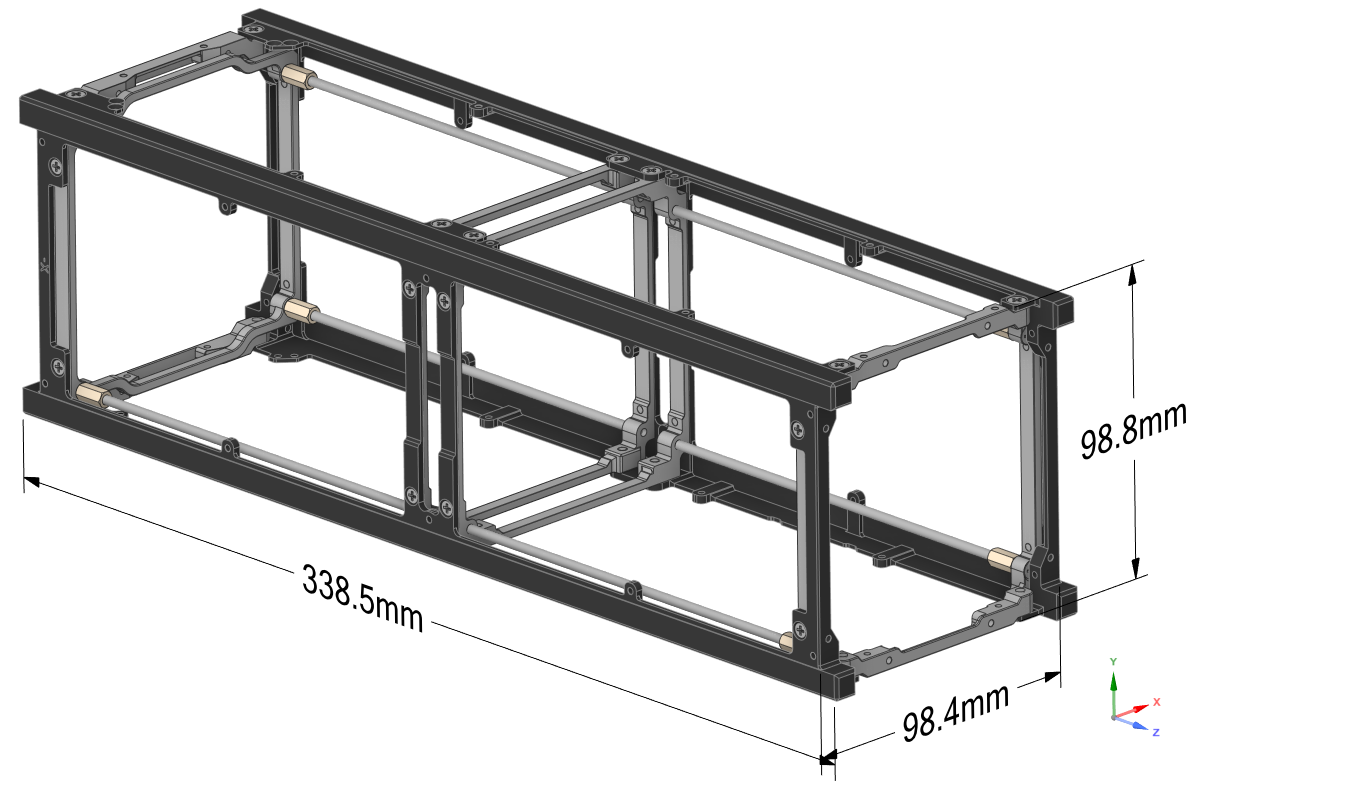
\includegraphics[scale=0.5]{fig/3Udims.png}
    \caption{3U cubesat structure with dimensions}
    \label{fig:3Udims}
\end{figure}

Based on dimensions shown in figure \ref{fig:3Udims} thruster diameter has to be smaller than 98.4 millimeters in diameter. There have been RF ion thrusters designed for cubesat applications in the past that had diameters smaller than 10 cm. BUSEK company have developed a RF ion thruster named BIT-3 which is shown in figure \ref{fig:BIT3}. This thruster has a 3cm grid from which it gets its name. BIT-3 is slated to be launched into Lunar orbit aboard a 6U sized cubesat named LunarCube in near future. 

\begin{figure}[ht]
    \centering
    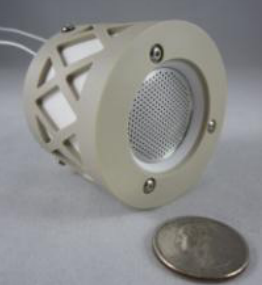
\includegraphics[scale=.8]{fig/BIT3.png}
    \caption[BIT-3 next to US 1\$ coin]{BIT-3 next to US 1\$ coin\cite{tsay2015lunarcube}}
    \label{fig:BIT3}
\end{figure}

BUSEK has also developed a smaller thruster called BIT-1 shown in figure \ref{fig:BIT1}. This thruster is designed to support Laser Interferometer Space Antenna(LISA) mission set to launch in 2037. Primary purpose of BIT-1 is to provide precise attitude control\cite{tsay2012micro}. 

\begin{figure}[ht]
    \centering
    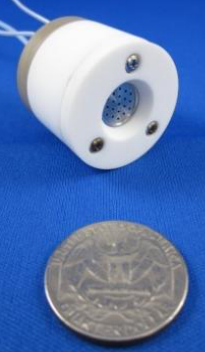
\includegraphics{fig/BIT1.png}
    \caption[BIT-1 next to US 1\$ coin]{BIT-1 next to US 1\$ coin\cite{tsay2012micro}}
    \label{fig:BIT1}
\end{figure}

Based on BUSEK's work and size of cubesat structure, sizing limitations for thruster are set to be between 10 millimeters to 98.4 millimeters. Considering the mechanical manufacturing convenience it was decided that overall thruster diameter shall be 94 millimeters. All subsystems of thruster have been designed accordingly. 
% RIT series developed by Giessen University and BIT series developed by BUSEK company can be shown as examples. 

\section{Plasma Generation System}
Plasma generation system consists of an RF coil to broadcast the signal and a discharge chamber to contain plasma as mentioned earlier in chapter \ref{ch:2_background}. 
\subsection{Discharge Chamber}
Material for discharge chamber is chosen as glass due to its ease of handling and accesibility. It was designed to consist wide and thin sections. Thin section will act as a channel through which the propellant will be fed into the wide section. Plasma will be created and sustained within the wide section. Approximate dimensions of discharge chamber is listed in table \ref{table:DC_params}. CAD and manufactured model of discharge chamber can be seen in figures \ref{fig:DC_cad} and \ref{fig:DC_real}. Approximations are the result of the relatively high manufacturing tolerances of glass production. 

\begin{table}[ht]
    \centering
    \begin{tabular}{||c|c||}
        \hline
        \textbf{Parameter} & \textbf{Approximate Value(mm)} \\
        \hline
        Total Length & 122 \\
        \hline
        Thin Section Lenght & 65 \\
        \hline
        Thin Section Outer Diameter & 6.35 \\
        \hline
        Wide Section Lenght & 57 \\
        \hline
        Wide Section Outher Diameter & 40 \\
        \hline
        Overall Thickness & 2 \\
        \hline
    \end{tabular}
    \caption{Parameters of Discharge Chamber}
    \label{table:DC_params}
\end{table}
 
\begin{figure}[ht]
    \centering
    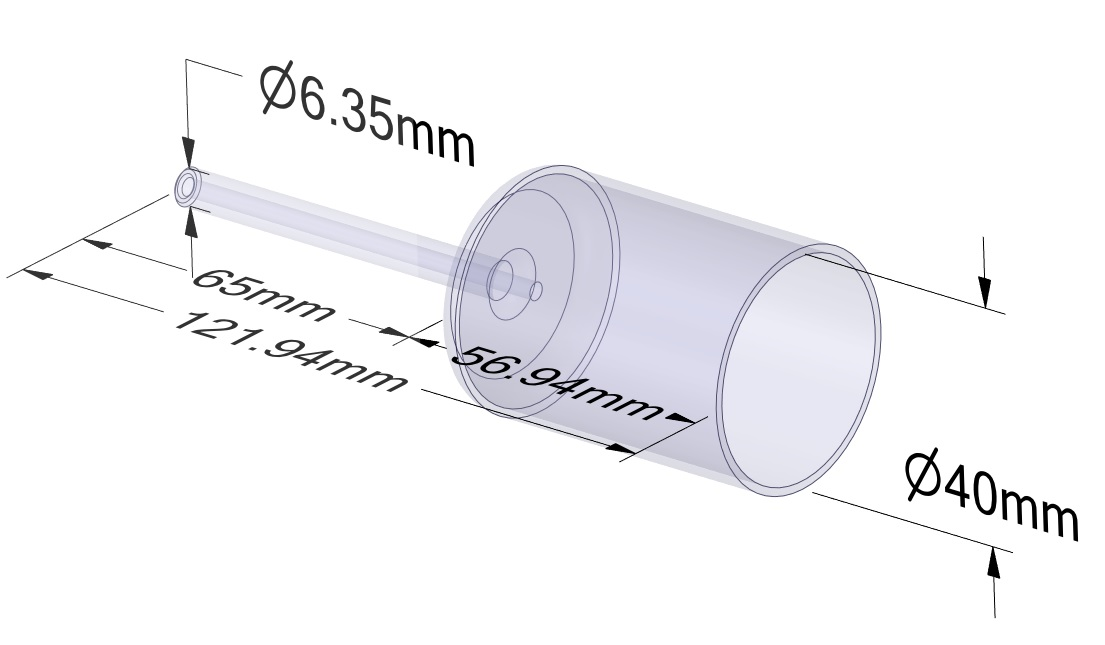
\includegraphics[scale=.45]{fig/DC_CAD.jpg}
    \caption{CAD of discharge chamber}
    \label{fig:DC_cad}
\end{figure}

\begin{figure}[ht]
    \centering
    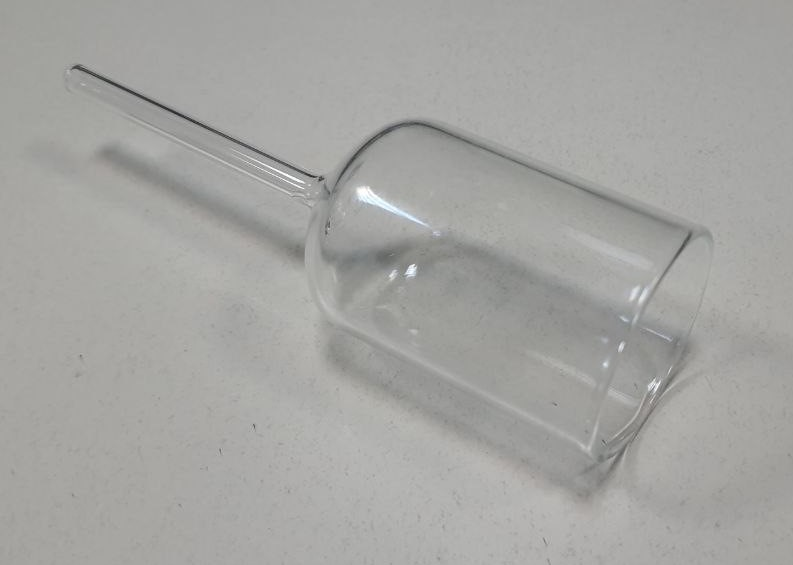
\includegraphics[scale=.35]{fig/DC_real.jpeg}
    \caption{Real model of discharge chamber}
    \label{fig:DC_real}
\end{figure}

\newpage
\subsection{RF Coil}
Due to skin depth effect RF signal is carried close to conductive material surface. Material selection for RF coil is made as copper. At 13.56MHz skin depth of copper is calculated to be 17.7$\mu$m\cite{bowick2011rf}. This fact allows the use of a tube instead of a solid transmission line. Using a tube is beneficial since it saves from material and it can be easily shaped into a coil. Parameters regarding the coil is given in table \ref{table:RFcoil_params}. CAD and real models of coil can be seen in figures \ref{fig:coil_CAD} and \ref{fig:coil_real}.
\newpage
\begin{table}[ht]
    \centering
    \begin{tabular}{||c|c||}
        \hline
        \textbf{Parameter} & \textbf{Value} \\
        \hline
        Inner Diameter & 4.7 mm\\
        \hline
        Outer Diameter & 2 mm \\
        \hline
        Overall length & 78.2 mm \\
         \hline
        Number of Turns & 5 \\
        \hline
    \end{tabular}
    \caption{Parameters of RF Coil}
    \label{table:RFcoil_params}
\end{table}

\begin{figure}[ht]
    \centering
    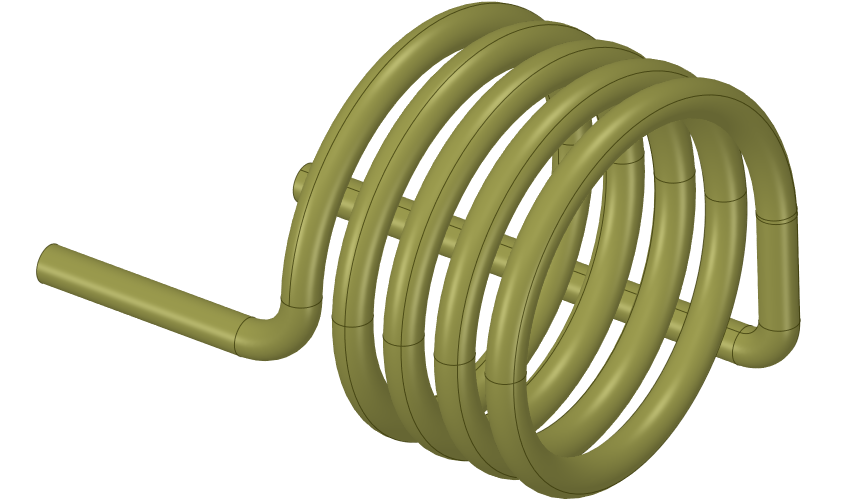
\includegraphics[scale=0.35]{fig/coil_CAD.png}
    \caption{CAD of RF coil}
    \label{fig:coil_CAD}
\end{figure}

\begin{figure}[ht]
    \centering
    \includegraphics[scale=0.35]{fig/realcoil.jpeg}
    \caption{RF coil}
    \label{fig:coil_real}
\end{figure}

\subsubsection{Coil Impedance}

Impedance is defined as the resistance of a conductor to the alternating current flowing through the said conductor. It is defined as the cumulative   effect of theresistance and reactance values of the circuit and similar to the resistance it is defined in ohm ($\Omega$) SI units. It is dependent on operating frequency.

Impedance value of the RF coil is important. A mismatch between the impedance values of the source and load, in this case RF coil, greatly hampers signal transmission. Details regarding the impedance mismatch and matching networks is provided in chapter \ref{ch:Ch4_mn}.\\

Impedance value measurements of the RF coil is performed via Siglent SVA 1032X Signal \& Vector Network Analyzer (VNA). Measurements can be displayed on the Smith chart. Smith chart is a circular shaped tool that is divided into inductive and capacitive regions shown in figure \ref{fig:smith_ex}. The impedence value measurements are inscripted onto the chart based on its imaginary (reactance) and real (resistance) values. Based on the reading an electrical circuit can be easily designed to bring the impedance value reading to the center of the Smith chart thus match the signal. 

\begin{figure}
    \centering
    \includegraphics{fig/smithchart_ex.png}
    \caption{Smith chart with descriptions}
    \label{fig:smith_ex}
\end{figure}
\newpage
RF coil is connected to the vector network analyzer's trace generation port via a split RF cable as shown in figure \ref{fig:antenna_meas}.

\begin{figure}[ht]
    \centering
    \includegraphics[scale=0.3,angle=90]{fig/antenna_meas.jpeg}
    \caption{Antenna connection to VNA}
    \label{fig:antenna_meas}
\end{figure}

Impedance value is measured at 13.56MHz. Result is shown in figure \ref{fig:smithchart_meas}

\begin{figure}[ht]
    \centering
    \includegraphics[scale=0.75]{fig/smithchart_meas.png}
    \caption{Impedance measurement of the RF coil}
    \label{fig:smithchart_meas}
\end{figure}
 
As can be seen from figure \ref{fig:smithchart_meas} impedance value for RF coil is far from ideal and an antenna tuner is needed.

\newpage
\section{Ion Extraction System} 
A pair of grids made out of stainless steel is designed and manufactured to act as the ion extraction system. In order to achieve optimum perveance, distance between grids and aperture diameters of screen and accel grids have to be determined. Literature survey on previous missions that include RF ion thrusters has been conducted to serve as a basis for grid distancing and aperture sizing. Results are provided in graph form in figure \ref{fig:farnellgrids}. 

\begin{figure}[ht]
    \centering
\includegraphics{fig/farnellgrids.png}
\caption[Geometrical parameters of RF ion grids in various missions]{Geometrical parameters of RF ion grids in various missions\cite{farnell2007performance}}
\label{fig:farnellgrids}
\end{figure}

Additionally grid parameters of BURFIT-80 have been taken into account since the thruster is proven to perform nominally. Based on these informations thicknesses of both grids have been determined to be 0.5 millimeters. Aperture diameteres of screen and accel grids are set to be 2.2 millimeters and 1.2 millimeters respectively. Distance between grids is set to be 1 millimeters.
\newpage
Laser cutting have been used to manufacture the grids. Four sets of pairs with different aperture numbers and different types of steel have been designed. For each grid an ear-like protrusion have been added to ease accesibility for electrical connections. Parameters, CAD and real model of first set of pairs is shown in table \ref{table:params_firstset}, figures \ref{fig:cad_firstset} and \ref{fig:real_firstset} respectively.

\begin{table}[ht]
    \centering
    \begin{tabular}{||c|c|c||}
        \hline
        \textbf{Parameter} & \textbf{Screen Grid} & \textbf{Accel. Grid} \\
        \hline
        Material & Steel SS304 & Steel SS304 \\
        \hline
        Outer diameter & 32 mm & 32 mm \\
        \hline
        Number of apertures & 91 & 91 \\
        \hline
        Aperture diameter & 2.2 mm & 1.2 mm \\
        \hline
        Thickness & 0.5 & 0.5 \\
        \hline
        Center-to-center distance between apertures & 3.2 mm & 3.2 mm \\
        \hline      
    \end{tabular}
\caption{Parameters of first set of grids}
\label{table:params_firstset}
\end{table}

\begin{figure}[ht]
    \centering
    \includegraphics[scale=.3]{fig/screen_6_cad.png}
    \includegraphics[scale=.3]{fig/accel_6_cad.png}
    \caption{CAD of screen(\textit{left)} and accel(\textit{right}) grids belonging to first set}
    \label{fig:cad_firstset}
\end{figure}

\begin{figure}[ht]
    \centering
    \includegraphics[scale=.08]{fig/screen_6_real.jpg}
    \includegraphics[scale=.08]{fig/accel_6_real.jpg}
    \caption{Real model of screen(\textit{left)} and accel(\textit{right}) grids belonging to first set}
    \label{fig:real_firstset}
\end{figure}

\newpage

Second set of grids with decreased number of apertures have been designed in order to ease manufacturing process and possibly reduce imperfections caused by production. Parameters, CAD and real model of first set of pairs is shown in table \ref{table:params_firstset}, figures \ref{fig:cad_firstset} and \ref{fig:real_firstset} respectively.

\begin{table}[ht]
    \centering
    \begin{tabular}{||c|c|c||}
        \hline
        \textbf{Parameter} & \textbf{Screen Grid} & \textbf{Accel. Grid} \\
        \hline
        Material & Steel SS304 & Steel SS304 \\
        \hline
        Outer diameter & 32 mm & 32 mm \\
        \hline
        Number of apertures & 61 & 61 \\
        \hline
        Aperture diameter & 2.2 mm & 1.2 mm \\
        \hline
        Thickness & 0.5 & 0.5 \\
        \hline
        Center-to-center distance between apertures & 4.2 mm & 4.2 mm \\
        \hline      
    \end{tabular}
\caption{Parameters of second set of grids}
\label{table:params_secondset}
\end{table}

\begin{figure}[ht]
    \centering
    \includegraphics[scale=.25]{fig/screen_5_cad.png}
    \includegraphics[scale=.25]{fig/accel_5_cad.png}
    \caption{CAD of screen(\textit{left)} and accel(\textit{right}) grids belonging to second set}
    \label{fig:cad_secondset}
\end{figure}

\begin{figure}[ht]
    \centering
    \includegraphics[scale=.35]{fig/screen_5_real.jpeg}
    \includegraphics[scale=.37]{fig/accel_5_real.jpeg}
    \caption{Real model of screen(\textit{left)} and accel(\textit{right}) grids belonging to second set}
    \label{fig:real_secondset}
\end{figure}

After the manufacture of first two sets imperfections, burrs and scorch marks have been observed around the apertures of the grids which are shown in figures \ref{fig:imperfect1} and \ref{fig:imperfect2}. 

\begin{figure}[ht]
    \centering
    \includegraphics[scale=0.25]{fig/imperfect2.jpeg}
    \caption{Imperfections on grids}
    \label{fig:imperfect1}
\end{figure}

\begin{figure}[ht]
    \centering
    \includegraphics[scale=0.25]{fig/imperfect1.jpeg}
    \caption{Close-up on imperfections on grids}
    \label{fig:imperfect2}
\end{figure}
\newpage
These imperfections are the result of usage of oxygen in the laser cutting process. Imperfections increase the risk of arc forming between grids when high voltage is introduced. In order to get rid of such impurities two additional sets, third and fourth, have been manufactured using a more durable kind of steel, SS316, and nitrogen instead of oxygen during laser cutting.  Apart from the differences in manufacturing process, parameters of third and fourth sets are identical to first and seconds sets respectively.

\begin{figure}[ht]
    \centering
    \includegraphics[scale=0.25]{fig/imperfect3.jpeg}
    \caption{Close-up on grids manufactured by nitrogen laser cutting}
    \label{fig:imperfect3}
\end{figure}

Result of nitrogen laser cutting is shown in figure \ref{fig:imperfect3} which shows a clear improvement regarding imperfections. Summary of designed grid parameters is provided in table \ref{table:gridparamsum}

\begin{table}[ht]
    \centering
    \begin{tabular}{||p{2cm}|p{2.2cm}|p{2.2cm}|p{2.5cm}|p{2.5cm}|p{2.7cm}||}
        \hline
        \textbf{Grid Set} & \textbf{Material} & \textbf{Number of Apertures} & \textbf{Screen Grid Aperture Dia.} & \textbf{Accel Grid Aperture Dia.} & \textbf{Distance Between Grids} \\
        \hline
        First Set & SS304 Steel & 91 & 2.2 mm & 1.2 mm & 1 mm \\
        \hline
        Second Set & SS304 Steel & 61 & 2.2 mm & 1.2 mm & 1 mm \\
        \hline
        Third Set & SS316 Steel & 91 & 2.2 mm & 1.2 mm & 1 mm \\
\hline
Fourth Set & SS316 Steel & 61 & 2.2 mm & 1.2 mm & 1 mm\\
\hline
    \end{tabular}
    \caption{Grid design parameters summary}
    \label{table:gridparamsum}
\end{table}
% \section{Support Structure}

\section{Thruster Assembly}
Grids, discharge chamber and RF coil are assembled together as shown in figures \ref{fig:thrusterassmgencad} and \ref{fig:thrusterassmgenreal}.

\begin{figure}[ht]
    \centering
    \includegraphics[scale=0.35]{fig/assm/assm_general.png}
    \caption{CAD of thruster assembly}
    \label{fig:thrusterassmgencad}
\end{figure}


\newpage

Exploded view of thruster design and explanation for each element is shown in figure \ref{fig:thrusterassmexp}. 

\begin{figure}[ht]
    \centering
    \includegraphics[width=\linewidth]{fig/assm/assm_exploded_ps.png}
    \caption{Exploded CAD of thruster}
    \label{fig:thrusterassmexp}
\end{figure}



As shown in figure \ref{fig:thrusterassmexp} there are numerous support elements to attach elements together. 
Spacers are used to electrically insulate grids from each other. Also in order to avoid arc forming from the sides grid covers are placed around the grids. Both spacers and
grid covers are made out of MICA, a dielectric, material. Grids and spacers are sandwiched between top and bottom structral plates. Bottom plate is made out of AL6061 to provide a strong backplate for grid assembly. Top plate is made out of teflon material which is light and durable. Six M3 sized screws keep the grids, spacers and structral plates together. In order to avoid electrically shorting the grids a specific type of screw made out of zirconia is used. They are tightened with M3 nuts as shown in figure \ref{fig:screwsreal}. 

% as shown in figure \ref{fig:screwsreal}. 

\begin{figure}[ht]
    \centering
    \includegraphics[width=\linewidth]{fig/assm/real_screws.jpg}
    \caption{Grid assembly fixed in place}
    \label{fig:screwsreal}
\end{figure}

Individual spacers, grid covers and teflon plate is shown in figure \ref{fig:realelements}.

\begin{figure}[ht]
    \centering
    \includegraphics[height=4cm]{fig/assm/real_cover.jpg}
    \includegraphics[height=4cm]{fig/assm/real_spacer.jpg}
    \includegraphics[height=4cm]{fig/assm/real_teflon.jpg}
    \caption{Grid cover, spacer and teflon plate}
    \label{fig:realelements}
\end{figure}
\newpage
Aluminum plate is glued to the glass discharge chamber using WURTH glass-metal glue as shown in figure \ref{fig:glass_alum}. 

\begin{figure}[ht]
    \centering
    \includegraphics[scale=.5]{fig/assm/al_glass.jpeg}
    \caption{Discharge chamber glued to aluminum backplate}
    \label{fig:glass_alum}
\end{figure}
\newpage
Electrical connectors are attached to the grids through the sides as shown in .figure \ref{fig:gridcons}. Thruster is then mounted onto a aluminum stand as shown in figure \ref{fig:backplate}. This aluminum stand has holes that antenna and discharge chamber feed line passes through.
\newpage
\begin{figure}[ht]
    \centering
    \includegraphics[width=0.8\linewidth]{fig/assm/real_gridcon.jpg}
    \includegraphics[width=0.8\linewidth]{fig/assm/real_gridcon2.jpg}
    \caption{Electrical connections to grids}
    \label{fig:gridcons}
\end{figure}


\begin{figure}[ht]
    \centering
    \includegraphics[width=0.8\linewidth]{fig/assm/real_backplate.jpg}
    \caption{Discharge chamber feed line and RF coil extensions}
    \label{fig:backplate}
\end{figure}

\newpage
Four M4 sized rods connect grid assembly and discharge chamber to the backplate to complete the assembly as shown in figure \ref{fig:thrusterassmgenreal} 

\begin{figure}[ht]
    \centering
    \includegraphics[width=\linewidth]{fig/assm/real_assm.png}
    \caption{Thruster assembly}
    \label{fig:thrusterassmgenreal}
\end{figure}
 \newpage
Additionally a steel mesh is wrapped around the thruster to contain broadcasted RF signals. This mesh is kept in place by a pair of plastic zip-ties as shown in figure \ref{fig:mesh}.

\begin{figure}[ht]
    \centering
    \includegraphics[width=\linewidth]{fig/assm/assm_mesh.jpg}
    \caption{Steel mesh wrapped aroung the thruster assembly}
    \label{fig:mesh}
\end{figure}

CAD of thruster assembly within a 3U cubesat chassis is shown in figure \ref{fig:3u_inside}. 

\begin{figure}[ht]
    \centering
    \includegraphics[width=\linewidth]{fig/3Udims_inside_iso.png}
    \caption{Thruster placed inside a 3U cubesat structure}
    \label{fig:3u_inside}
\end{figure}


\newpage

\section{Calculations}
Based on background information given in chapter \ref{ch:2_background} and design parameters provided earlier in this chapter calculations have been performed to predict thrust and $I_{sp}$ values. 
\subsection{Thrust Calculations}
In order to calculate thrust values first charge density of ion beam have to calculated which was given in equation \ref{eq:childlangmuir}. For the sake of calculations it is beneficial to restate the charge density equation. 

\begin{equation}
    J = \frac{4}{9}\varepsilon_0 \sqrt{\frac{2e}{m_i}}\frac{V^{\frac{3}{2}}_B}{l_{e}^2}
    \label{eq:childlangch3}
\end{equation}

where $J$ is the current density with units of $A/m^2$, $e$ is the value of electric charge, $\varepsilon_0$ is the permittivity of free space, $l_e$ is the ion acceleration distance, $m_i$ is the mass of ion in terms of kilograms and $V$ is the total voltage used to accelerate ions. Ion acceleration distance $l_e$ is highly dependent on the accelerator grid parameters, summary of which is provided in the table \ref{table:gridparams}.

\begin{table}[ht]
    \centering
    \begin{tabular}{||c|c||}
        \hline
        \textbf{Parameter} & \textbf{Value} \\
        \hline
        Screen Grid Thickness($T_s$) & 0.5 mm \\
        \hline
        Accel. Grid Thickness($T_a$) & 0.5 mm \\
        \hline
        Distance Between Grids($l_g$) & 1 mm \\
        \hline
        Screen Grid Aperture Diameter($D_s$) & 2.2 mm \\
        \hline
        Accel. Grid Aperture Diameter($D_a$) & 1.2 mm \\
        \hline
        Number of Apertures & 91 \\
        \hline
    \end{tabular}
    \caption{Grid Parameters}
    \label{table:gridparams}
\end{table}

$l_e$ is calculated using equation \ref{eq:acceldistance}

\begin{equation}
    l_e =  \sqrt{(l_g + T_s)^2 + \frac{D_{s}^2}{4}}
    \label{eq:acceldistance}
\end{equation}

Using the parameters listed in table \ref{table:gridparamsum} the ion acceleration distance is calculated as 1.86 mm.

Grid voltages are arbitrarily chosen as +800V for screen grid and -200V for acceleration grid. Not all of this potential is transferred to the ion beam. Sum of total voltages used to polarize the grids is named as total voltage whereas voltage transferred to the ion beam is named beam voltage. Their relation is shown as\cite{farnell2007performance};

\begin{equation}
    R = \frac{V_B}{V_T} = \frac{V_B}{V_s + |V_a|}
    \label{eq:Rvalue}
\end{equation}

where $V_s$ and $V_a$ are screen and grid potentials respectively. R value usually ranges between 0.85 to 0.9\cite{farnell2007performance}. For the remainder of this study it will be assumed as 0.85. From this assumption total voltage $V_T$ is calculated as 1000V and subsequently beam voltage $V_B$ is calculated as 850V. 
In this study the propellant is selected as Argon which has atomic mass unit of 39.948 daltons which is equal to 6.63E-26 kg. Inputting the parameters listed above into the equation \ref{eq:childlangch3} the ion beam current density is calculated as 78.82 $A/m^2$. This charge density is distributed over the active area of the grids which is defined as the total aperture area of the grid. For active area calculations active area of the screen grid is taken into account since it is the grid that limits the ion beam flow. 91 apertures with 2.2 mm diameter each gives 345.92 $mm^2$. Dividing the ion beam current density to active area gives the ion beam current as 27.26 mA. This beam current value is put into the thrust equation which is given as 

\begin{equation}
    T = \sqrt{\frac{2m_i V_B}{q}} I_b
    \label{eq:thrustereq}
\end{equation}

Based on equation \ref{eq:thrustereq} the thrust is given as 784.57 $\mu N$. This value does not take beam divergence or doubly charged ion loss into account. Assuming 10\% doubly charge ion ratio and 10 degree ion beam divergence the value of the thrust decreases to 752.07 $\mu N$. Relation of thrust levels versus beam potential is shown in figure \ref{chart:thrustlevels}.

\begin{figure}[ht]
\centering   
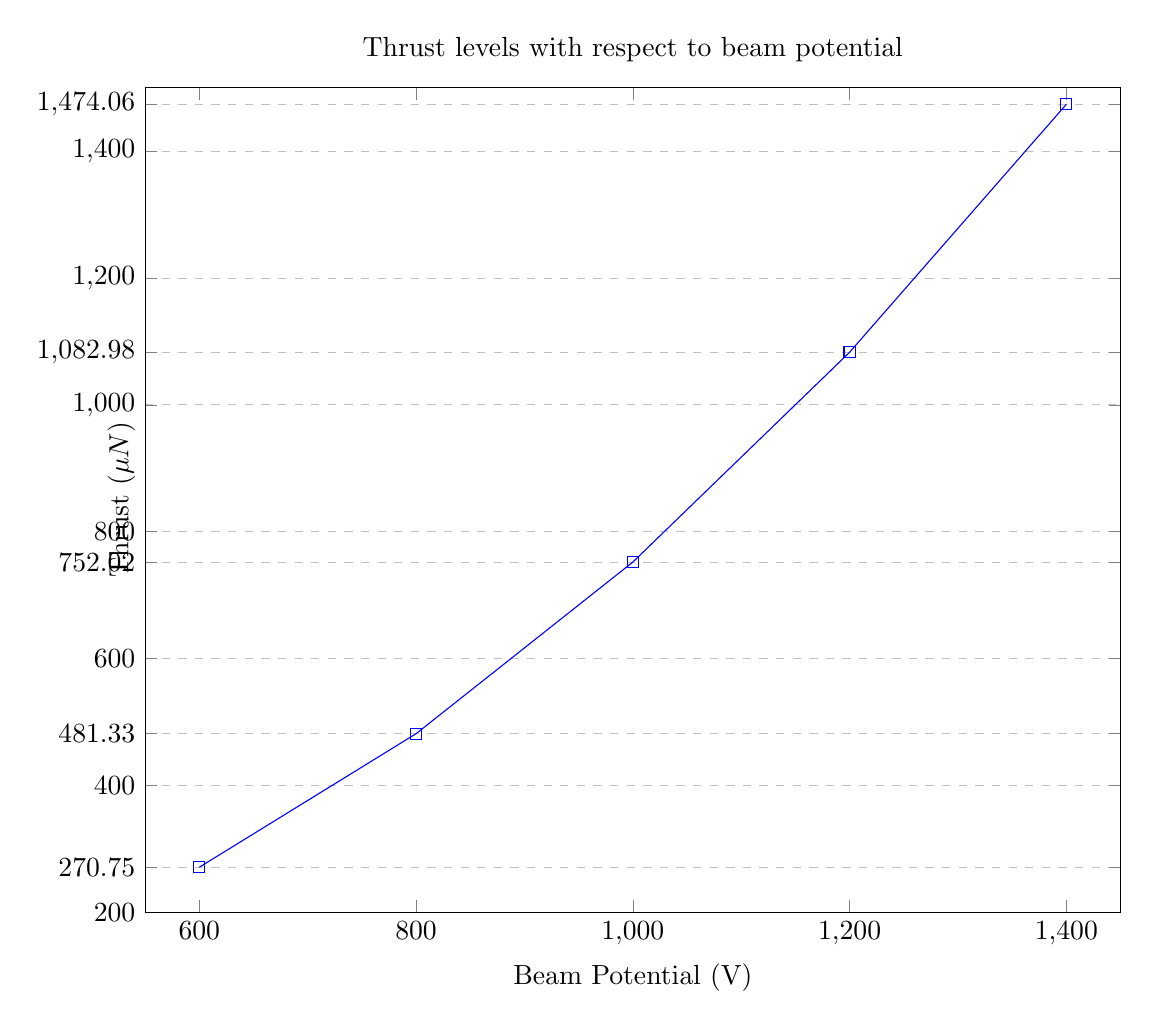
\begin{tikzpicture}
    \pgfplotsset{width=5.5in}
    \begin{axis}[
        title={Thrust levels with respect to beam potential},
        xlabel={Beam Potential (V)},
        y label style={at={(axis description cs:0,.5)}, anchor=south},
        ylabel={Thrust ($\mu N$)},
        xmin=550, xmax=1450,
        ymin=200, ymax=1500,
        xtick={600, 800, 1000, 1200, 1400},
        ytick={200, 270.75, 400, 481.33, 600, 752.02, 800, 1000, 1082.98, 1200, 1400, 1474.06},
        legend pos=north west,
        ymajorgrids=true,
        grid style=dashed,
    ]
        \addplot[
        color=blue,
        mark=square,
        ]
        coordinates {
        (600,270.75)(800,481.33)(1000,752.02)(1200,1082.98)(1400,1474.06)
        };
    \end{axis}
    \end{tikzpicture}
    \caption{Thrust Levels With Respect to Beam Potential}
    \label{chart:thrustlevels}
\end{figure}

As can be seen in figure \ref{chart:thrustlevels} provided thrust levels increase exponentially with increasing beam voltage. 

\newpage
\subsection{Specific Impulse Calculations}

Specific impulse value is given as 

\begin{equation}
    I_{sp} = \gamma \frac{\eta_m}{g} \sqrt{\frac{2qV_b}{m_i}}
\end{equation}

Inserting the values of $\gamma$, $g$ and $q$;

\begin{equation}
    I_{sp} = 1.417 \times 10^3 \eta_m \sqrt{\frac{V_B}{m_i}}
\end{equation}

where $\eta_m$ is the mass utilization efficiency; ratio of ionized propellant to unionized propellant. Similar to thrust calculations assumptions are; doubly charged ion ratio is  as 10\%, ion beam divergence of 10 degrees and 850V beam voltage with argon propellant. Calculated specific impulse values with respect to mass utilization efficiency and beam potential is shown in figure \ref{chart:isplevels}

\begin{figure}[ht]
    \centering   
    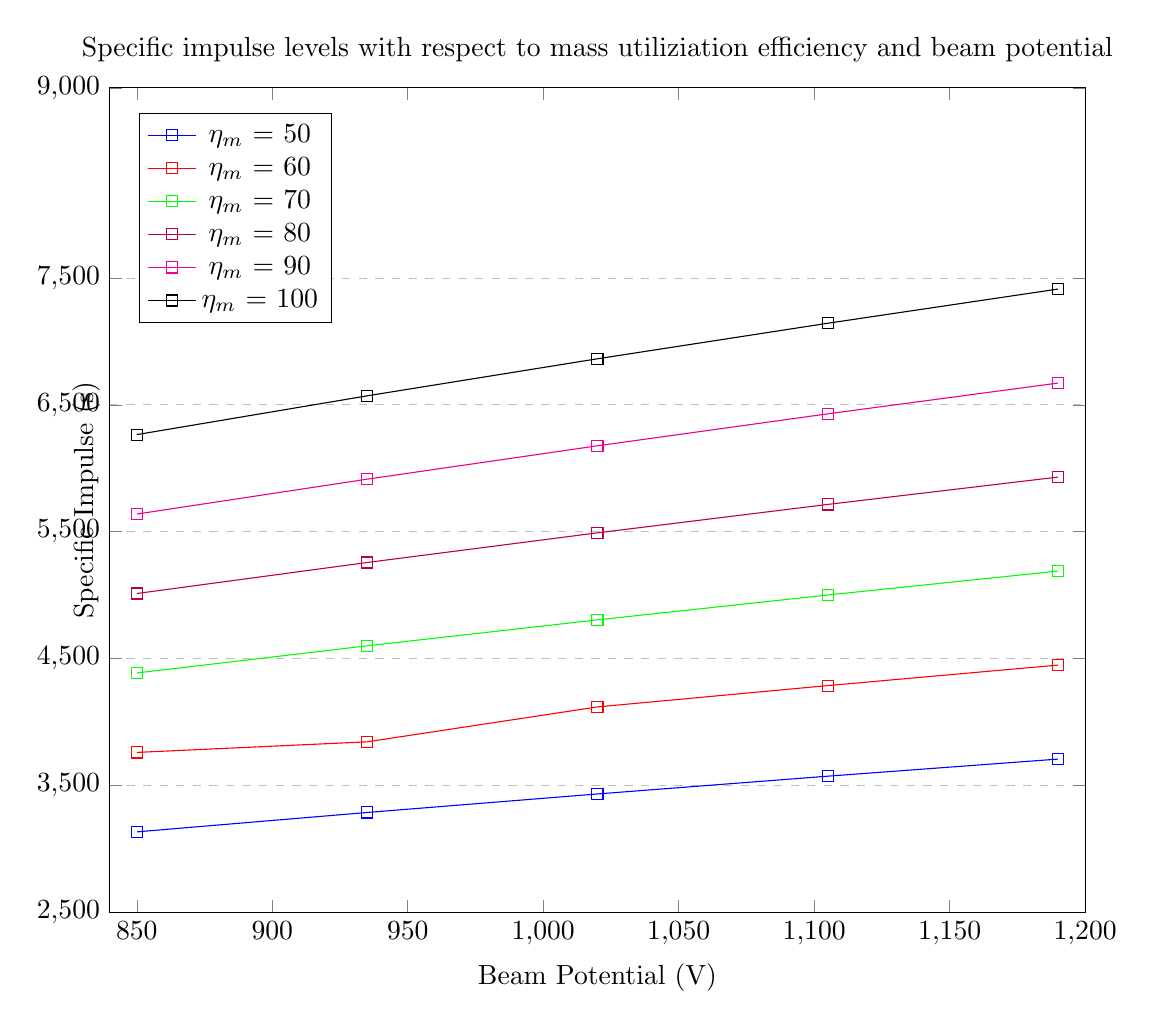
\begin{tikzpicture}
        \pgfplotsset{width=5.5in}
        \begin{axis}
            [
            title={Specific impulse levels with respect to mass utiliziation efficiency and beam potential},
            xlabel={Beam Potential (V)},
            y label style={at={(axis description cs:0,.5)}, anchor=south},
            ylabel={Specific Impulse (s)},
            xmin=840, xmax=1200,
            ymin=2500, ymax=9000,
            xtick={800, 850, 900, 950, 1000, 1050, 1100, 1150, 1200},
            ytick={2500, 3500, 4500, 5500, 6500, 7500, 9000},
            legend pos=north west,
            ymajorgrids=true,
            grid style=dashed,
        ]
            \addplot[
            color=blue,
            mark=square,
            ]
            coordinates {
            (850,3132.77)(935,3285.68)(1020,3431.78)(1105,3571.91)(1190,3706.74)
            };
            \addlegendentry{$\eta_m$ = 50}
            \addplot[
            color=red,
            mark=square,
            ]
            coordinates {
            (850,3759.32)(935,3842.81)(1020,4118.13)(1105,4286.29)(1190,4448.09)
            };
            \addlegendentry{$\eta_m$ = 60}
            \addplot[
            color=green,
            mark=square,
            ]
            coordinates {
            (850,4385.88)(935,4599.95)(1020,4804.49)(1105,5000.67)(1190,5189.44)
            };
            \addlegendentry{$\eta_m$ = 70}
            \addplot[
                color=purple,
                mark=square,
                ]
                coordinates {
                (850,5012.43)(935,5257.08)(1020,5490.84)(1105,5715.05)(1190,5930.79)
                };
                \addlegendentry{$\eta_m$ = 80}
                \addplot[
                    color=magenta,
                    mark=square,
                    ]
                    coordinates {
                    (850,5638.98)(935,5914.22)(1020,6177.2)(1105,6429.43)(1190,6672.14)
                    };
                    \addlegendentry{$\eta_m$ = 90}
                    \addplot[
                        color=black,
                        mark=square,
                        ]
                        coordinates {
                        (850,6265.54)(935,6571.35)(1020,6863.55)(1105,7143.81)(1190,7413.48)
                        };
                        \addlegendentry{$\eta_m$ = 100}
        \end{axis}
        \end{tikzpicture}
        \caption{$I_{sp}$ levels with respect to $\eta_m$ and $V_B$}
        \label{chart:isplevels}
    \end{figure}
    



% \subsection{1st Prototype}
% \subsection{2nd Prototype}

 
% \subsection{Page Margins}


% The gap at the bottom of the page is 2.5 cm. 

% Keeping more redundant space is incorrect. So, this gap should not be. Texts, tables, figures, etc. in the pages must be arranged considering this situation.

% \section{RF System Design}




% % ---------------------------------------------------------------- %
% % Numbered citation.						                       %
% % ---------------------------------------------------------------- %


%%%%%%%%%%%%%%%%%%%%%%%%%%%%%%%%%%%%%%%%%%%%%%%%%%%%%%%%%%%%%%%%%
\chapter{EXPERIMENTAL SETUP AND METHODOLOGY}\label{Ch:Ch4_expsetup}
%%%%%%%%%%%%%%%%%%%%%%%%%%%%%%%%%%%%%%%%%%%%%%%%%%%%%%%%%%%%%%%%%
Experiments were performed in the vacuum chamber at the BUSTLab of Bogazici University. The laboratory contains a vacuum chamber, AC and DC power supplies, network matching circuits, propellant container tanks, propellant flow lines and flow controller. Ion beam charge density and divergence is measured by a Faraday cup which is in-house built by members of BUSTLab\cite{yildiz2019plume}. By measuring the beam charge density deductions about produced thrust levels can be made. \\
Majority of experimental setup was manually operated. Ion beam measurement system was controlled by LabVIEW software. In this chapter experimental setup and its elements will be explained. Experimental procedures and attempts at operating the thruster will be provided. 

\section{Experimental Setup}
\newpage
\subsection{Vacuum Chamber}
All experiments were performed in a custom built Kurt J. Lesker brand vacuum chamber shown in figure \ref{fig:bustlabchamber}. It has a diameter of 1.5 meters and lenght of 2.7 meters. It is primarily used to perform experiments with electric propulsion systems that use Argon or Xenon propellant. \\
\begin{figure}[ht]
    \centering
    \includegraphics[scale=0.1]{fig/bustlabchamber.jpg}
    \caption{BUSTLab vacuum chamber}
    \label{fig:bustlabchamber}
\end{figure}

The vacuum chamber can achieve high vacuum levels up to $10^{-8}$ torrs thanks to a mechanical and cryogenic pumps. This vacuum level is akin to low earth orbit vacuum levels which ranges between $10^{-7}$ to $10^{-9}$ torrs\cite{Horneck2011}. Vacuum chamber can sustain very low pressure levels even when a thruster is operating in chamber during which a propellant is continuously pumped into the chamber. 

% \begin{figure}[ht]
%     \centering
%     \includegraphics[scale=0.075]{fig/cryopump.jpg}
%     \includegraphics[scale=0.05]{fig/mechanicalpump.jpg}
%     \caption{Cryopump and mechanical pump}
%     \label{fig:bustpump}
% \end{figure}
\newpage
Thrust chamber allows access to the interior through feedthroughs. There are numerous feedthroughs with different sizes and purposes. One of them is used to connect the RF line from the signal source to thruster. Two feedthroughs are used to connect the gas feed. Several feedthroughs are used to connect the DC power lines. 

\begin{figure}[ht]
    \centering
    \includegraphics[height=5cm]{fig/dcfeedout.jpg}
    \includegraphics[height=5cm]{fig/RFfeedout.jpg}
    \includegraphics[height=5cm]{fig/gasfeedout.jpg}
    \caption{From top to bottom DC, RF and propellant feedthroughs}
    \label{fig:vacuumfeed}
\end{figure}
\newpage
\subsection{RF Power Supply}
RF power source is AG1213W type RF generator shown in figure \ref{fig:rfpowersup}. It can generate signals with up to 1200W of power. It outputs constant 13.56MHz frequency. It is suitable for industrial, scientific and medical applications.

\begin{figure}[ht]
    \centering
    \includegraphics[height=6cm]{fig/rfpowersup.jpg}
    \caption{RF power source}
    \label{fig:rfpowersup}
\end{figure}

A LED screen displays set output power, forwarded power, load power and reflected power. Through load and reflected power impedence mismatch can be determined which will be discussed in the following subsection.

\subsection{Matching Network} \label{ch:Ch4_mn}
Since RF coil will used to broadcast a signal its impedance value carries a significance. Impedance is the opposition of alternating current(AC) flow which carries the RF signal\cite{slurzberg1950essentials}. It is represented with SI unit of ohm($\Omega$). If there is an impedence mismatch between the source and the antenna then signal transmission is significantly hindered. Usually commercial and industrial RF products are manufactured to have a default of 50$\Omega$ impedance. For example signal source used for this product, AG1213W, is defaulted to 50$\Omega$ of impedence.

Since RF coil used in this work is specifically designed for this thruster, its impedence is not compatible with that of RF power source's. In order to match the impedence value of the antenna, or load, to signal generator, or source, an electronic circuit is introduced to the system. This process is called network matching. For this work Palstar AT2K 2000W network tuner, shown in figure \ref{fig:tuner}, is used to match the network.

\begin{figure}[ht] 
    \centering
    \includegraphics[height=6cm]{fig/tuner.jpg}
    \caption{Network tuner}
    \label{fig:tuner}
\end{figure}

This tuner consists of two variable capacitors and a variable inductor. Two capacitors are connected in series and the inducter is connected in parallel(shunt) to complete the circuit. On the front side of the tuner is an SWR (standing wave ratio) meter which shows reflected and forwarded power similar to the RF signal source. Based on this SWR meter transmitted signal power is determined. 

Types and working mechanisms of matching networks are explained in detail in appendix \ref{ch:appndxB_RF}.
% In this section, information will be given about how citations, quotings and footnotes should be.
\subsection{DC Power Supplies}
Two DC power supplies, one for each grid, are needed. There are three DC power supplied present within the laboratory. Two of them are Sorenson brand, models DCS60-18E and DCS600-1.7E which can output 60V-18A and 600V-1.7A respectively. Third power supply is Glassman brand and can provide 1500V-1.5A. They are shown in figure \ref{fig:dcpowersups}.

\begin{figure}[ht] 
    \centering
    \includegraphics[height=6cm]{fig/dcpowersups.jpeg}
    \caption{DC Power supplies}
    \label{fig:dcpowersups}
\end{figure}

\subsection{Propellant Feed Line and Flow Controller}
Argon propellant is kept at pressurized tanks. Flow rate of propellant into the discharge chamber is important and is controlled by a MKS PR4000B type flow controller shown in figure \ref{fig:flowcont}. It displays the flow are in units of cubic centimeters per minute (SCCM). 

\begin{figure}[ht]
    \centering
    \includegraphics[height=7cm]{fig/flowcontroller.jpeg}
    \caption{Flow controller}
    \label{fig:flowcont}
\end{figure}

A feedthrough is used to drive the propellant lines through vacuum chamber as shown in figure \ref{fig:propfeedthr}. There are two feed lines are present. Feedline 1 can support flow rates up to 25 SCCMs whereas feedline 2 can support flowrates up to 1000 SCCMs.

\begin{figure}[ht]
    \centering
    \includegraphics[height=5cm]{fig/propfeedthr.jpeg}
    \caption{Propellant feedthrough}
    \label{fig:propfeedthr}
\end{figure}



% \subsection{Methodology}
% \section{Citing (indication of references in main text body)}
% \section{Input Parameters}

% \subsection{Citing according to surname of author}

% References are cited with the surname of author and year. In the references section, the references are listed alphabetically according to the surname of the author.

% Citing of a reference at the beginning of or within a sentence must be as Boran (2003), whereas a citation at the end of a sentence must be as (Boran, 2003). The full-stop is placed directly after the citation.
 
% A reference with two authors must be cited as Yılmaz and Johnson (2004) at the beginning of or within a sentence, or as (Yılmaz and Johnson, 2004) at the end of a sentence. 

% A reference with more than two authors must be cited as Yılmaz et al. (2004) at the beginning of or within a sentence, or as (Yılmaz et al, 2004) at the end of a sentence. 

% Different publications of an author published in the same year must be cited as Feray (2005a), Feray (2005b). 

% While citing a part of a publication; the number of the page the cited material (chapter, table, figure, or equation) is on must be indicated. While citing, the expression “page” must be abbreviated, but “chapter” must not. For example; (Centers for Disease Control and Prevention, 2005, p. 10), (Shimamura, 1989, Chapter 3). 

% Citing multiple publications in one pair of brackets; (Berndt, 2002; Harlow, 1983). 

% Citing personal communication in main text body; (V.–G. Nguyen, personal communication, September 28, 1998), (J. Smith, personal communication, August 15, 2009).

% In the references section, reference tags must be listed according to the surname of author. 

% For citing of secondary references (In case the reference cites another reference), the secondary reference must be cited in brackets.  In the references section, the reference tag is organized according to the secondary reference, the original reference must not be used as a tag. For example; In his e-mails, Smith argued that asynchronous line dancing would be the next Internet meme (as cited in Jones, 2010).

% \subsection{Citing according to order of appearance}

% References are cited by numbering and indicating the number in square brackets ([]) in the main text body. The first reference cited in a thesis is numbered [1] and the following references are numbered according to the order of appearance. 

% In the main text body, references must be cited as specified below:
% \vspace*{-12pt}
% \begin{tabbing}
% \hspace*{1.5cm}\= \kill
% [1]      \> Reference no. 1\\

% [1--3]   \> References from no.1 to 3 (thus, references 1,2 and 3)\\

% [1,3]    \> References no. 1 and 3\\

% [1,3,8]  \> References no.1, 3 and 8\\

% [1,3--8] \> References no.1, and from no.3 to 8 (thus, references 1, 3, 4, 5, 6, 7 and 8)
% \end{tabbing}
% \vspace*{-12pt}
% Different volumes of a reference must be cited and numbered individually.
\newpage
\section{Experimental Procedure}
% \subsection{Thruster Placement}
% \subsection{Faraday Cup Placement}
A number of firing tests were conducted using systems described above. Thruster is placed inside the vacuum chamber. It was placed on a makeshift table in order to make it easier to observe through the windows of the vacuum chamber. Placement of the thruster is shown in figure \ref{fig:invacuum_assm}.

\begin{figure}[h]
    \centering
    \includegraphics[scale=0.15]{fig/invacuum_assembly.jpg}
    \caption{Thruster within the vacuum chamber}
    \label{fig:invacuum_assm}
\end{figure}

RF signal is carried to the thruster via RG 393 cable. RF and DC connection cables were run through feedthroughs of the vacuum chamber and connected to the thruster via clamps. Propellant feed line is connected to the narrow end of the discharge chamber. All connections are shown in \ref{fig:invacuum_accel}, \ref{fig:invacuum_screen} and \ref{fig:invacuum_rf}. 
\newpage
\begin{figure}[h]
    \centering
    \includegraphics[scale=0.12]{fig/invacuum_accel.jpg}
    \caption{Connections of acceleration grid}
    \label{fig:invacuum_accel}
\end{figure}

\begin{figure}[h]
    \centering
    \includegraphics[scale=0.12]{fig/invacuum_screen.jpg}
    \caption{Connections of screen grid}
    \label{fig:invacuum_screen}
\end{figure}
\newpage
\begin{figure}[h]
    \centering
    \includegraphics[scale=0.1]{fig/invacuum_rf.jpg}
    \caption{Connections of RF coil and propellant feedline}
    \label{fig:invacuum_rf}
\end{figure}

At this point impedance value of the RF coil is measured again.  It was discovered that the ground of the RF feedthrough is shorted to the entire vacuum chamber which created a different impedance value reading compared to the original measurements of the RF coil previously shown in figure \ref{fig:smithchart_meas}. Results of the new measurement is shown in figure \ref{fig:smithchar_meas_comb}.

\begin{figure}[h]
    \centering
    \includegraphics[scale=0.5]{fig/antenna_meas_combined.jpeg}
    \caption{Impedance value of coil combined with vacuum chamber}
    \label{fig:smithchar_meas_comb}
\end{figure}

Antenna tuner is included within the circuit to match the impedance values. Total circuit schematic is shown in figure \ref{fig:schematic}.

\begin{figure}[ht]
    \centering
    \includegraphics{fig/thrusterschematic.jpeg}
    \caption{Experimental setup schematic}
    \label{fig:schematic}
\end{figure}

After setting up the thruster a series of ignition tests were performed. Effect of different ion extractor grid, propellant flow rate, RF and DC power levels were examined throughout the tests. Initial tests failed due to number of reasons. Tests were conducted until a steady stream of ions were observed leaving the thruster. 

\newpage
\subsection{Firing Test No. 1}
During the first test pressure inside the vacuum chamber has been reduced down to $1.8x10^{-5}$ torrs. For this test ion extractor grids were made out of SS304 grade steel and they were manufactured using oxygen laser cutting process. Center to center distance of grid apertures were 3.2 mm and there were a total of 91 apertures. Signal between the RF source and antenna have been tuned to provide 1.02 SWR. Plasma inside the discharge chamber have been succesfully ignited with 5W of RF power and 13 SCCM propellant flow rate as shown in figure \ref{fig:1st_ccp}. Ignited plasma is observed to be capacitively coupled plasma (CCP) judging by the low power input and faint glow of plasma. 

\begin{figure}[ht]
    \centering
    \includegraphics[width=\linewidth]{fig/deneme1/test1_ccp.jpg}
    \caption{CCP formed within the thruster during first firing test}
    \label{fig:1st_ccp}
\end{figure}

After initial ignition RF power have been increased to 30W and screen and acceleration grids have been polarized with ground and +1000V potential respectively. It has been observed that increased RF power has caused plasma to transit to inductively coupled plasma (ICP). After the grids are polarized bright flashes have been observed forming between grids and potentials of the grids have begun to fluctuate indicating that an electical arc is forming between grids. Propellant flow rate has been increased to 25 SCCM to increase the number of ions within the discharge chamber but unfortunately electical arc has continued to form. Excess propellant escaping the thruster has coupled with the RF antenna and created a dim glow within the vacuum chamber as shown in figure \ref{fig:1st_icp}.
\newpage

\begin{figure}[ht]
    \centering
    \includegraphics[width=\linewidth]{fig/deneme1/test1_discharge.jpg}
    \caption{Thruster during first firing test}
    \label{fig:1st_icp}
\end{figure}

Note that in figure \ref{fig:1st_icp} the plume exiting the thruster is not an ion beam but merely excess non-ionized propellant escaping the thruster.
At this stage test has been aborted. The failure and electical arc forming are attributed to the mechanical roughness and imperfections of the grids as shown in figure \ref{fig:1st_imperfect}. These imperfections are determined to be the result of the oxygen laser cutting process. Additionally after the test is complete the thruster is disassembled and it was discovered that a spacer plate between grids was missing due to human error. This resulted in a sub-optimal ion optics configuration.

\begin{figure}[ht]
    \centering
    \includegraphics[scale=0.3]{fig/imperfect1.jpeg}
    \caption{Grid imperfections during first firing test}
    \label{fig:1st_imperfect}
\end{figure}

Decision has been made to remove the imperfections by hand using mechanical file prior to second firing tests.
\newpage
\subsection{Firing Test No. 2}
Before attempting to fire the thruster for the second time the ion extraction grids are extensively filed using fine sandpiper to remove roughness and imperfections. Filed grids are shown in figure \ref{fig:2nd_grids_before}. Afterwards the thruster is assembled properly with and experimental setup has been completed as described earlier. 

\begin{figure}[ht]
    \centering
    \includegraphics[width=0.4\linewidth]{fig/deneme2/test2_screen_before.jpg}
    \includegraphics[width=0.41\linewidth]{fig/deneme2/test2_accel_before.jpg}
    \caption{Screen(\textit{left}) and acceleration(\textit{right}) grids before second firing test}
    \label{fig:2nd_grids_before}
\end{figure}

Prior to test the pressure level of the vacuum chamber has been reduced to $2.39x10^{-4}$ torrs. Similar to first firing test plasma has been succesfully ignited as CCP with 5W of RF power and 13 SCCM propellant flow rate. RF power level has been steadily increased to 45W and ICP has been achieved as shown in figure \ref{fig:2nd_icp}. 

\begin{figure}[ht]
    \centering
    \includegraphics[width=\linewidth]{fig/deneme2/test2_icpglow.jpg}
    \caption{ICP during second firing test}
    \label{fig:2nd_icp}
\end{figure}

After ICP is acquired the screen and acceleration grids have been polarized with ground and +600V of potential respectively. It was observed that despite extensive mechanical filing impurities of grids continued to cause electrical short between grids. In figure \ref{fig:2nd_short} a bright flash can be seen due to forming of electrical arcs. 

\begin{figure}[ht]
    \centering
    \includegraphics[width=\linewidth]{fig/deneme2/test2_short.jpg}
    \caption{Electrical short during second firing test}
    \label{fig:2nd_short}
\end{figure}

The test has been aborted at this point. After disassembling the thruster severe degragation of ion accelerator grids has been discovered as shown in figure \ref{fig:2nd_grids_after}.

\begin{figure}[ht]
    \centering
    \includegraphics[width=0.41\linewidth]{fig/deneme2/test2_screen_after.jpg}
    \includegraphics[width=0.4\linewidth]{fig/deneme2/test2_accel_after.jpg}
    \caption{Screen(\textit{left}) and acceleration(\textit{right}) grids after second firing test}
    \label{fig:2nd_grids_after}
\end{figure}

\newpage
\subsection{Firing Test No. 3}
For third attempt a new set of grids with increased center to center distance between apertures have been designed and manufactured. Manufacturing process was again oxygen laser cutting. Center to center distance have been increased to 4.2mm for third firing test. This resulted the number of apertures to decrease from 91 to 61. Areas around the apertures have been filed using DRAMEL device. Grids after filing are shown in figure \ref{fig:3rd_grids_before}.

\begin{figure}[ht]
    \centering
    \includegraphics[width=0.41\linewidth]{fig/deneme3/test3_screen_before.jpeg}
    \includegraphics[width=0.4\linewidth]{fig/deneme3/test3_accel_before.jpeg}
    \caption{Screen(\textit{left}) and acceleration(\textit{right}) grids used in third firing test}
    \label{fig:3rd_grids_before}
\end{figure}

Purpose of this change in aperture center to center distance is to keep arcs from forming between apertures. Thruster is assembled and experimental setup has been established normally. During the test the pressure level inside vacuum chamber has been reduceed to $1.34x10^{-4}$ torrs. RF input power and propellant flow rate have been set to 30W and 12 SCCM respectively.     
Screen grid and acceleration grid have been polarized with ground and -600V respectively. Plasma inside the thruster has transited to ICP at approximately 60W of RF power. 
Despite increased center to center distance between apertures and even extensive filing electrical arcs have been observed to continue forming. Test has been aborted. It was decided to seek alternate methods for grid production in order to completely eliminate burrs and impurities during manufacturing process. 
\newpage
\subsection{Firing Tets No. 4}
A new set of grids have been manufactured. This time nitrogen was used during laser cutting. Grid materal have also been changed. Instead of SS304, SS316 grade steel was used for the fourth test. These changes resulted in a much more robust and smooth ion extractor grids as shown in figure \ref{fig:4th_grids_before}. 

\begin{figure}[ht]
    \centering
    \includegraphics[width=0.41\linewidth]{fig/deneme4/test4_screen_before.jpg}
    \includegraphics[width=0.4\linewidth]{fig/deneme4/test4_accel_before.jpg}
    \caption{Screen(\textit{left}) and acceleration(\textit{right}) grids before in fourth firing test}
    \label{fig:4th_grids_before}
\end{figure}

RF power has been set to 10W and propellant flow rate was set 13 SCCM. Plasma ignition was succesfully achieved in CCP. RF power has been increased gradually until ICP is acheieved as shown in figure \ref{fig:4th_icp}. Transition from CCP to ICP has occured around 80W which is the highest level at which the ICP has been achieved so far. 

\begin{figure}[ht]
    \centering
    \includegraphics[width=\linewidth]{fig/deneme4/test4_icp.jpeg}
    \caption{ICP during fourth firing test}
    \label{fig:4th_icp}
\end{figure}

Initally screen and acceleration grid potentials were set to +1000V and ground potential respectively. This configuration yielded no ions and introduced slight arcing. Potentials were changed to +600V for screen grid and -200V. This change still yielded no accelerated ions but reduced the occurence frequency of arcs. Afterwards screen grid potential was increased to +800V while acceleration grid potential was kept at -200V. Under this configuration forming of a single beamlet from one of the apertures was observed as shown in 
figure \ref{fig:4th_single}.
\begin{figure}[ht]
    \centering
    \includegraphics[scale=0.4]{fig/deneme4/test4_singlebeam.jpeg}
    \caption{Single ion beam forming}
    \label{fig:4th_single}
\end{figure}

At this point it was concluded that the arcing problem between grids was resolved. RF power has been increased to 120W and ion beams from the rest of the apertures have been observed to form as shown in figure \ref{fig:4th_multi}. 

\begin{figure}[ht]
    \centering
    \includegraphics[scale=0.4]{fig/deneme4/test4_multibeam.jpeg}
    \caption{Multiple ion beam forming}
    \label{fig:4th_multi}
\end{figure}

This stage marks the first proper successful ion acceleration and discharge. Changing experimental parameters; RF power, flow rate, grid potentials offered no improvements to ion beam forming. Since there is no equipment in place to measure ion beam plume characteristics and thrust no measurements were taken. Test was deemed a success. After the test the thruster was disassembled and grids were examined. Scorch marks and degragation on the grids are clearly visible as shown in figure \ref{fig:4th_grideg}.

\begin{figure}[ht]
    \centering
    \includegraphics[width=0.4\linewidth]{fig/deneme4/test4_screen_after.jpg}
    \includegraphics[width=0.4\linewidth]{fig/deneme4/test4_accel_after.jpg}
    \caption{Screen(\textit{left}) and acceleration(\textit{right}) grids after in fourth firing test}
    \label{fig:4th_grideg}
\end{figure}



% \section{Quoting}

% Generally, quoting is done by remaining faithful to the original text in terms of words, spelling and punctuation. In case there is a mistake, the correct version is written in square brackets in the quoted text.

% Short quotations (not longer than 40 words) must be given in quotation marks. Following the text quoted, the reference must be written and a full-stop must be placed afterwards.  

% Quotations longer than 40 words must not be shown in quotation  marks. Instead, they must be indented 1 tab space (1.27 cm) from the left side of the page. The font size for long quotations indented from the left must be 2 pt smaller than the font size used in main text body. However, it is not advised to quote very long texts and to quote very frequently. Unlike short quotations, references of long quotations must be placed after the full stop. (i.e., .(p.196))

% Example for a quotation at the beginning of a sentence;

% According to Jones (1998), "Students often had difficulty using APA style,  especially when it was their first time" (p. 199).

% Example for a quotation in the middle of a sentence;

% Interpreting these results, Robbins et al. (2003) suggested that the “therapists in dropout cases may have inadvertently validated parental negativity about the adolescent without adequately responding to the adolescent’s needs or concerns” (p. 541) contributing to an overall climate of negativity.

% Example for a quotation at the end of a sentence;

% Confusing this issue is the overlapping nature of roles in palliative care, whereby “medical needs are met by those in the medical disciplines; nonmedical needs may be addressed by anyone on the team” (Csikai \& Chaitin, 2006, p. 112). 

% Detailed information on quoting could be found on websites of Graduate Schools and associated links.

% \section{Footnotes}

% Footnotes could be used in theses to add content-expanding, content-enhancing, or additional information. 
% Footnote numbers must be placed directly after a quotation. In case the quotation is a paragraph, the footnote numbers must be placed directly after the last word of the paragraph (as superscript). In case the quotation is a concept or a noun, footnote numbers must be placed directly after that concept or noun (as superscript). 

% Footnote numbers in the main text body must be indicated as superscript, as shown\footnotemark. A punctuation mark must not be placed after the number.

% Footnotes must be written with a font size 2 pt smaller than the main text body font size.
 
% 1 space must be set between footnote line and footnote number, 1/2 space must be set between footnote number and the first line of the footnote. Footnotes must be separated from the main text body with a thin horizontal line. 

% Detailed information on footnotes could be found on the websites of Graduate Schools and associated links.

% \footnotetext{~Reference display can not be done with footnotes.~Footnotes could be used in theses to add content-expanding, content-enhancing, or additional information.~If these information must include references, these references must be indicated in References section.}

% \section{Second Level Title: First Letters Capital}

% \subsection{Third level title: Only first letter capital}


% \subsubsection{Fourth level title: Only first letter capital}



% \subsubsubsection{Fifth level title: No numbering after fourth level titles}



% % Include tilda to provide one letter spacing between the foot number and the text at the bottom - SBÖ
% \footnotetext{~~Footnotes must be written with a font size 2 pt smaller than the main text body font size.}

% \begin{figure}[t]
% 	\centering
% 	\includegraphics[width=230pt,keepaspectratio=true]{./fig/sekil6}
% 	% sekil6.eps: 0x0 pixel, 300dpi, 0.00x0.00 cm, bb=14 14 555 489
% 	\caption{Example figure.}
% 	\label{Figure4.1}
% \end{figure}

% This indicates that the ANN is accurate at base flow and flow height values lower then 3 m. 

% \begin{table*}[h]
% 	{\setlength{\tabcolsep}{14pt}
% 		\caption{Example table.}
% 		\begin{center}
% 			\vspace{-6mm}
% 			\begin{tabular}{cccc}
% 				\hline \\[-2.45ex] \hline \\[-2.1ex]
% 				Column A & Column B & Column C & Column D \\
% 				\hline \\[-1.8ex]
% 				Row A & Row A & Row A & Row A \\
% 				Row B & Row B & Row B & Row B \\
% 				Row C & Row C & Row C & Row C \\
% 				[-0ex] \hline
% 			\end{tabular}
% 			\vspace{-6mm}
% 		\end{center}
% 		\label{Table4.1}}
% \end{table*}

%%%%%%%%%%%%%%%%%%%%%%%%%%%%%%%%%%%%%%%%%%%%%%%%%%%%%%%%%%%%%%%%%
\chapter{RESULTS \& DISCUSSION}\label{Ch5}
%%%%%%%%%%%%%%%%%%%%%%%%%%%%%%%%%%%%%%%%%%%%%%%%%%%%%%%%%%%%%%%%%

The RF ion thruster development study so far have achieved the following: plasma generation, plasma containing and sustaining, ion beam extraction. During majority of the testing stage the issue with plasma arcing has been tackled. The problem was solved using SS316 grade stainless steel and nitrogen laser cutting technique for grid production. Unfortunately ion beam characteristics have not been measured. At this stage only predictions and calculations can be done regarding the thrust levels produced by the thruster. 

In this chapter approximate thrust and specific impulse levels will be calculated using equations depicted in chapter \ref{ch:2_background} and experimental parameters provided in chapter \ref{Ch:Ch4_expsetup}. During tests the thruster could only be operated on the fourth test. Experimental and physical parameters during the fourth test are summarized in the table \ref{table:predictionparams} below.

\begin{table}[ht]
    \centering
    \begin{tabular}{||c|c||}
        \hline
        \textbf{Parameter} & \textbf{Value} \\
        \hline
        RF Power & 80 W \\
        \hline
        Screen Grid Voltage & +800 V \\
        \hline
        Accel. Grid Voltage & -200 V \\
        \hline 
        Propellant Flow Rate & 12 sccm \\
        \hline
        Screen Grid Diameter & 2.2 mm \\
        \hline
        Accel. Grid Diameter & 1.2 mm \\
        \hline
        Distance Between Grids & 1 mm \\
        \hline
        Number of Apertures & 61 \\
        \hline
        Mass of Ion & 38.948 u \\
        \hline
    \end{tabular}
    \caption{Parameters used in thruster predictions}
    \label{table:predictionparams}
\end{table}
\newpage
\section{Thrust Predictions}

Thrust predictions are made using Child-Langmuir and thrust equations shown in previous chapters. In order to ease calculations they are shown below again. 
Equation \ref{eq:resultchild} displays Child-Langmuir equation for ion beam charge density. 

\begin{equation}
    J = \frac{4}{9}\varepsilon_0 \sqrt{\frac{2e}{m_i}}\frac{V_T^{\frac{3}{2}}}{d^2}
    \label{eq:resultchild}
\end{equation}

Equation \ref{eq:resultthrust} shown the thrust equation.

\begin{equation}
    T = \gamma \sqrt{\dfrac{2m_i V_b}{e}}I_b
    \label{eq:resultthrust}
\end{equation}

In early chapters assumptions were made regarding the $\gamma$ thrust correction factor. These assumptions were 10\% doubly charge ion ratio and 10 degree beam divergence. Taking these assumptions into account gives $\gamma$ value as 0.959. Using rest of the parameters listed in talbe \ref{table:predictionparams} ion beam charge density is calculated as 78.82 $A/m^2$. 61 apertures of the grids results in grid active area of 231.88 $mm^2$ thus the ion beam charge is calculated as 18.28 $mA$. Inputting all these values into the equation \ref{eq:resultthrust} gives 504.14 $\mu N$ of thrust.

\section{Specific Impulse Predictions}

Specific impulse formula is restated as 

\begin{equation}
    I_{sp} = \gamma \frac{\eta_m}{g} \sqrt{\frac{2qV_b}{m_i}}
    \label{eq:resultsisp}
\end{equation}

After inputting the appopriate parameters equation \ref{eq:resultsisp} turns into;

\begin{equation}
    I_{sp} = 6265.53  \eta_m
    \label{eq:resultsisp2}
\end{equation}

From equation \ref{eq:resultsisp2} it is evident that the specific impulse levels are dependent on mass utilization efficiency. Change in specific impulse levels with different mass utilization efficiency ratio is shown in table \ref{table:resultsispchart}.

\begin{table}
    \centering
    \begin{tabular}{||c|c||}
        \hline
        Mass Utilization Efficiency (\%) & $I_{sp}$ (s) \\
        \hline
        50 & 3132.76 \\
        \hline
        60 & 3759.32 \\
        \hline
        70 & 4385.87 \\
        \hline
        80 & 5012.43 \\
        \hline
        90 & 5638.98 \\
        \hline
        \end{tabular}
        \caption{Values for $I_{sp}$ with regards to mass utilization efficiency}
        \label{table:resultsispchart}
\end{table}

As shown in table \ref{table:resultsispchart} $I_sp$ values are predicted in the range of 3132.76 to 5638.98 seconds.

\newpage
% \section{Plume Diagnostics}
% \section{Comparison}
% \section{Efficiency Calculations}

% In this thesis, the necessary steps for constructing an end-to-end streamflow forecasting system were discussed. These steps include the use.

% \section{Second Level Title: First Letters Capital}


% \subsection{Third level title: Only first letter capital}


% \subsubsection{Fourth level title: Only first letter capital}


% %\newpage
% %{\bf Fifth level title: No numbering after fourth level titles}
% \subsubsubsection{Fifth level title: No numbering after fourth level titles}


% \begin{figure}
% 	\centering
% 	\includegraphics[width=230pt,keepaspectratio=true]{./fig/sekil5}
% 	% sekil5.eps: 0x0 pixel, 300dpi, 0.00x0.00 cm, bb=14 14 1193 701
% 	\vspace{3mm}
% 	\caption{Example figure in chapter 5.}
% 	\label{Figure5.1}
% \end{figure}

% This indicates that the ANN is accurate at base flow and flow height values lower then 3 m. 

% \begin{table*}[h]
% 	{\setlength{\tabcolsep}{14pt}
% 		\caption{Example table in chapter 5.}
% 		\begin{center}
% 			\vspace{-6mm}
% 			\begin{tabular}{cccc}
% 			    \hline \\[-2.45ex] \hline \\[-2.1ex]
% 				Column A & Column B & Column C & Column D \\
% 				\hline \\[-1.8ex]
% 				Row A & Row A & Row A & Row A \\
% 				Row B & Row B & Row B & Row B \\
% 				Row C & Row C & Row C & Row C \\
% 				[-0ex] \hline
% 			\end{tabular}
% 			\vspace{-6mm}
% 		\end{center}
% 		\label{Table5.1}}
% \end{table*}

 

%%%%%%%%%%%%%%%%%%%%%%%%%%%%%%%%%%%%%%%%%%%%%%%%%%%%%%%%%%%%%%%%%
\chapter{CONCLUSION AND FUTURE WORK}\label{Ch6}
%%%%%%%%%%%%%%%%%%%%%%%%%%%%%%%%%%%%%%%%%%%%%%%%%%%%%%%%%%%%%%%%%

In this study a compact RF ion thruster system was designed for cube satellite applications. Limitations emposed by cube satellite standards were briefly mentioned and literature research regarding the current state of the RF ion thruster technology was presented. Working principle of an RF ion thruster were explained. A detailed design study was then performed on the RF ion thruster. Limitations emposed by the cube satellite standards were given. Based on the design parameters calculations were performed to determine the amount of thrust and specific impulse the thruster can generate. 

A series of firing tests were then conducted in a vacuum chamber. Details about the experimental setup and environment were provided. Initial tests had resulted in failure due to mechanical complications within the ion accelerator grids of the thruster. These mechanical complications included the low production quality of the grids, imperfections and burrs left behind after laser cutting process. First three tests had resulted in an electrical short forming between grids and thus had failed. Material and production process of the grids were then changed. Eventually on the fourth test the thruster was operated as intended. 

Not all of research objectives were met. During experiments the thruster was observed to accelerate ions in the form of ion beamlets which is a visual indication of thrust generation. However due to lack of experimental setup no results regarding ion beam characteristics were recorded. A faraday probe, or cup, would be used to record the ion beam charge. Various types of faraday probes have been used in the studies electic propulsion systems to determine ion beam characteristics.


For this study a guardad planar type of faraday probe would be used. An exploded CAD view of the probe is provided in figure \ref{fig:explodedfaraday}.


\begin{figure}[ht]
    \centering
    \includegraphics[width=\linewidth]{fig/faradayprobeexploded.png}
    \caption[Exploded view of guarded planar Faraday probe]{Exploded view of guarded planar Faraday probe\cite{yildiz2019plume}}
    \label{fig:explodedfaraday}
\end{figure}

\newpage

The probe is enclosed in a cylindirical conductive cylinder called guard ring and a collector plate is positioned at the base of the probe. Conductive ring and the collector is polarised with the same potential as shown in figure \ref{fig:faradayschematic} to ensure that the ion collection only occurs on the collector plate. 

\begin{figure}[ht]
    \centering
    \includegraphics[scale=0.5]{fig/probeschematic.png}
    \caption[Working schematic of a guarded faraday probe]{Working schematic of a guarded faraday probe\cite{brown2017recommended}}
    \label{fig:faradayschematic}
\end{figure}


Probe would be positioned downstream of the ion beam and the opening of the probe would face the thruster so that the ions would enter the probe. Charge incurred on the collector plate would then be measured using a sourcemeter. This measurement would then be used to determine the amount of generated thrust. Faraday cup measurements would be performed in a hemispherical manner, as shown in figure \ref{fig:probepos}, which would also determine the beam divergence angle thus amount of lost thrust.

\begin{figure}[ht]
    \centering
    \includegraphics[scale=0.5]{fig/probepos.png}
    \caption[Faraday probe path and measurement points]{Faraday probe path and measurement points\cite{Couch2017}}
    \label{fig:probepos}
\end{figure}
\newpage

Another point for further study is to increase grid transparency in order to create more uniform ion beam out of created beamlets. This would increase the thrust generated by the ion thruster and also create a more visible ion beam. 

When the thruster was succesfully operated it was fitted with a grid with 61 apertures. Distance between apertures were 4.2 mm between each aperture. As future work thruster can be operated with a grid that has more closely located apertures. 

% \section{Practical Application of This Study}

% Lorem ipsum dolor sit amet, consetetur sadipscing elitr, sed diam nonumy eirmod tempor invidunt ut labore et dolore magna aliquyam erat, sed diam voluptua. At vero eos et accusam et justo duo dolores et ea rebum. Stet clita kasd gub rgren, no sea takimata sanctus est Lorem ipsum dolor sit amet, consetetur sadipscing elitr, sed diam nonumy eirmod tempor invidunt ut lab ore sit et dolore magna.

% \section{Second Level Title: First Letters Capital}


% \subsection{Third level title: Only first letter capital}

% \subsubsection{Fourth level title: Only first letter capital}


% This indicates that the ANN is accurate at base flow and flow height values lower then 3 m. 

% \begin{table*}[!htbp]
% 	{\setlength{\tabcolsep}{14pt}
% 		\caption{Example table in chapter 6.}
% 		\begin{center}
% 			\vspace{-6mm}
% 			\begin{tabular}{cccc}
% 				\hline \\[-2.45ex] \hline \\[-2.1ex]
% 				Column A & Column B & Column C & Column D \\
% 				\hline \\[-1.8ex]
% 				Row A & Row A & Row A & Row A \\
% 				Row B & Row B & Row B & Row B \\
% 				Row C & Row C & Row C & Row C \\
% 				[-0ex] \hline
% 			\end{tabular}
% 			\vspace{-6mm}
% 		\end{center}
% 		\label{Table6.1}}
% \end{table*}



% %{\bf Fifth level title: No numbering after fourth level titles}
% \subsubsubsection{Fifth level title: No numbering after fourth level titles}

% \begin{figure}
% 	\centering
% 	\includegraphics[width=230pt,keepaspectratio=true]{./fig/sekil7}
% 	% sekil7.eps: 0x0 pixel, 300dpi, 0.00x0.00 cm, bb=14 14 455 369
% 	\caption{Example table in chapter 6.}
% 	\label{Figure6.1}
% \end{figure}




% \chapter{APPENDIX A.1}
% \vglue6pt
% % For Appendix A.1
% % Format the equation environment
% \renewcommand{\theequation}{A.1.\arabic{equation}}
% % Reset the counter
% \setcounter{equation}{0}

% \begin{table*}[!ht]
% 	{\setlength{\tabcolsep}{14pt}
% 		\caption{Example table in appendix.}
% 		\begin{center}
% 			\vspace{-6mm}
% 			\begin{tabular}{cccc}
% 				\hline \\[-2.45ex] \hline \\[-2.1ex]
% 				Column A & Column B & Column C & Column D \\
% 				\hline \\[-1.8ex]
% 				Row A & Row A & Row A & Row A \\
% 				Row B & Row B & Row B & Row B \\
% 				Row C & Row C & Row C & Row C \\
% 				[-0ex] \hline
% 			\end{tabular}
% 			\vspace{-6mm}
% 		\end{center}
% 		\label{TableA.1}}
% \end{table*}

% \begin{equation}
% y_{t} = \phi_{1} y_{t-1} + \epsilon_{t}
% \label{EqA.1.1}
% \end{equation}

% Each parameter is described. As seen in equation \eqref{EqA.1.1}, or in \ref{EqA.1.1}.

% \begin{equation}
% y_{t} = \phi_{1} y_{t-1} + \epsilon_{t}
% \label{EqA.1.2}
% \end{equation}

% \vspace*{12pt}

% \section*{APPENDIX A.2}
% \vglue6pt
% % For Appendix A.2
% % Format the equation environment
% \renewcommand{\theequation}{A.2.\arabic{equation}}
% % Reset the counter
% \setcounter{equation}{0}


% \begin{equation}
% y_{t} = \phi_{1} y_{t-1} + \epsilon_{t}
% \label{EqA.2.1}
% \end{equation}

% Each parameter is described. As seen in equation \eqref{EqA.2.1}, or in \ref{EqA.2.1}.

% \newpage
% \chapter{APPENDIX B.1}
% \vglue12pt
% % For Appendix B.1
% % Format the equation environment
% \renewcommand{\theequation}{B.1.\arabic{equation}}
% % Reset the counter
% \setcounter{equation}{0}


% \begin{equation}
% y_{t} = \phi_{1} y_{t-1} + \epsilon_{t}
% \label{EqB.1.1}
% \end{equation}
% Each parameter is described. As seen in equation \eqref{EqB.1.1}, or in \ref{EqB.1.1}.

% \begin{equation}
% y_{t} = \phi_{1} y_{t-1} + \epsilon_{t}
% \label{EqB.1.2}
% \end{equation}

% Each parameter is described. As seen in equation \eqref{EqB.1.2}, or in \ref{EqB.1.2}.

% \begin{table*}[!ht]
% 	{\setlength{\tabcolsep}{14pt}
% 		\caption{Example table in appendix.}
% 		\begin{center}
% 			\vspace{-6mm}
% 			\begin{tabular}{cccc}
% 				\hline \\[-2.45ex] \hline \\[-2.1ex]
% 				Column A & Column B & Column C & Column D \\
% 				\hline \\[-1.8ex]
% 				Row A & Row A & Row A & Row A \\
% 				Row B & Row B & Row B & Row B \\
% 				Row C & Row C & Row C & Row C \\
% 				[-0ex] \hline
% 			\end{tabular}
% 			\vspace{-6mm}
% 		\end{center}
% 		\label{TableB.1}}
% \end{table*}

% \vspace*{18pt}

% \section*{APPENDIX B.2}
% \vglue6pt
% % For Appendix B.2
% % Format the equation environment
% \renewcommand{\theequation}{B.2.\arabic{equation}}
% % Reset the counter
% \setcounter{equation}{0}


% \begin{equation}
% y_{t} = \phi_{1} y_{t-1} + \epsilon_{t}
% \label{EqB.2.1}
% \end{equation}

% Each parameter is described. As seen in equation \eqref{EqB.2.1}, or in \ref{EqB.2.1}.

% \begin{table*}[!ht]
% 	{\setlength{\tabcolsep}{14pt}
% 		\caption{Example table in appendix.}
% 		\begin{center}
% 			\vspace{-6mm}
% 			\begin{tabular}{cccc}
% 				\hline \\[-2.45ex] \hline \\[-2.1ex]
% 				Column A & Column B & Column C & Column D \\
% 				\hline \\[-1.8ex]
% 				Row A & Row A & Row A & Row A \\
% 				Row B & Row B & Row B & Row B \\
% 				Row C & Row C & Row C & Row C \\
% 				[-0ex] \hline
% 			\end{tabular}
% 			\vspace{-6mm}
% 		\end{center}
% 		\label{TableB.2}}
% \end{table*}

% \chapter{APPENDIX A: CHILD-LANGMUIR EQUATION}

% \chapter{APPENDIX B: RF SYSTEM DESIGN} \label{ch:appndxB_RF}
% \chapter{APPENDIX C: FARADAY CUP} 
% \chapter{APPENDIX A: RF SYSTEM DESIGN}\label{Ch7}
% \chapter{APPENDIX B: FARADAY CUP}\label{Ch8}

% ----------------------------------------------------------------- %
% Form thesis_bib.bib to contain your references in bibtex format   %
% use \cite command for citing your references.                     %
% ----------------------------------------------------------------- %

\bibliographystyle{thesis_itubib}      % Designed .bst file 
\bibliography{thesis_bib}			   % .bib file

% ----------------------------------------------------------------- %
% Appendix files. appendices_cover is the appendix title page.      %
% ----------------------------------------------------------------- %

\eklerkapak{}
%\vglue18pt  % This has to be 18 pt - SBÖ
\singlespacing
% \textbf{APPENDIX A.1 :} Example table and equations in the Appendices\\
% \textbf{APPENDIX A.2 :} Additional information provided in the Appendices\\
% \textbf{APPENDIX B.1 :} More additional information provided in the Appendices\\
% \textbf{APPENDIX B.2 :} More and more additional information provided in the Appendices\\

% One way of implementing multiple appendix in a row is to use itemize as in below to prevent issues on the indentation in the second line.

\begin{itemize}[leftmargin=3.3cm,itemsep=-0.4em,labelsep=1.5mm] % Adust margin to flush left, item sep., label sep. - SBÖ
\item [\textbf{APPENDIX A.1 :}]RF system design
\item [\textbf{APPENDIX A.2 :}]Faraday cup
% \item [\textbf{APPENDIX B.1 :}]More additional information provided in the Appendices
% \item [\textbf{APPENDIX B.2 :}]More and more additional information provided in the Appendices can go to the second line
\end{itemize}



\newpage

% ----------------------------------------------------------------- %
% \eklerbolum{x} forms and appendix of x chapters. 				    %
% ----------------------------------------------------------------- %

\eklerbolum{0}
% \chapter{APPENDIX A.1}
% \vglue6pt
% % For Appendix A.1
% % Format the equation environment
% \renewcommand{\theequation}{A.1.\arabic{equation}}
% % Reset the counter
% \setcounter{equation}{0}

% \begin{table*}[!ht]
% 	{\setlength{\tabcolsep}{14pt}
% 		\caption{Example table in appendix.}
% 		\begin{center}
% 			\vspace{-6mm}
% 			\begin{tabular}{cccc}
% 				\hline \\[-2.45ex] \hline \\[-2.1ex]
% 				Column A & Column B & Column C & Column D \\
% 				\hline \\[-1.8ex]
% 				Row A & Row A & Row A & Row A \\
% 				Row B & Row B & Row B & Row B \\
% 				Row C & Row C & Row C & Row C \\
% 				[-0ex] \hline
% 			\end{tabular}
% 			\vspace{-6mm}
% 		\end{center}
% 		\label{TableA.1}}
% \end{table*}

% \begin{equation}
% y_{t} = \phi_{1} y_{t-1} + \epsilon_{t}
% \label{EqA.1.1}
% \end{equation}

% Each parameter is described. As seen in equation \eqref{EqA.1.1}, or in \ref{EqA.1.1}.

% \begin{equation}
% y_{t} = \phi_{1} y_{t-1} + \epsilon_{t}
% \label{EqA.1.2}
% \end{equation}

% \vspace*{12pt}

% \section*{APPENDIX A.2}
% \vglue6pt
% % For Appendix A.2
% % Format the equation environment
% \renewcommand{\theequation}{A.2.\arabic{equation}}
% % Reset the counter
% \setcounter{equation}{0}


% \begin{equation}
% y_{t} = \phi_{1} y_{t-1} + \epsilon_{t}
% \label{EqA.2.1}
% \end{equation}

% Each parameter is described. As seen in equation \eqref{EqA.2.1}, or in \ref{EqA.2.1}.

% \newpage
% \chapter{APPENDIX B.1}
% \vglue12pt
% % For Appendix B.1
% % Format the equation environment
% \renewcommand{\theequation}{B.1.\arabic{equation}}
% % Reset the counter
% \setcounter{equation}{0}


% \begin{equation}
% y_{t} = \phi_{1} y_{t-1} + \epsilon_{t}
% \label{EqB.1.1}
% \end{equation}
% Each parameter is described. As seen in equation \eqref{EqB.1.1}, or in \ref{EqB.1.1}.

% \begin{equation}
% y_{t} = \phi_{1} y_{t-1} + \epsilon_{t}
% \label{EqB.1.2}
% \end{equation}

% Each parameter is described. As seen in equation \eqref{EqB.1.2}, or in \ref{EqB.1.2}.

% \begin{table*}[!ht]
% 	{\setlength{\tabcolsep}{14pt}
% 		\caption{Example table in appendix.}
% 		\begin{center}
% 			\vspace{-6mm}
% 			\begin{tabular}{cccc}
% 				\hline \\[-2.45ex] \hline \\[-2.1ex]
% 				Column A & Column B & Column C & Column D \\
% 				\hline \\[-1.8ex]
% 				Row A & Row A & Row A & Row A \\
% 				Row B & Row B & Row B & Row B \\
% 				Row C & Row C & Row C & Row C \\
% 				[-0ex] \hline
% 			\end{tabular}
% 			\vspace{-6mm}
% 		\end{center}
% 		\label{TableB.1}}
% \end{table*}

% \vspace*{18pt}

% \section*{APPENDIX B.2}
% \vglue6pt
% % For Appendix B.2
% % Format the equation environment
% \renewcommand{\theequation}{B.2.\arabic{equation}}
% % Reset the counter
% \setcounter{equation}{0}


% \begin{equation}
% y_{t} = \phi_{1} y_{t-1} + \epsilon_{t}
% \label{EqB.2.1}
% \end{equation}

% Each parameter is described. As seen in equation \eqref{EqB.2.1}, or in \ref{EqB.2.1}.

% \begin{table*}[!ht]
% 	{\setlength{\tabcolsep}{14pt}
% 		\caption{Example table in appendix.}
% 		\begin{center}
% 			\vspace{-6mm}
% 			\begin{tabular}{cccc}
% 				\hline \\[-2.45ex] \hline \\[-2.1ex]
% 				Column A & Column B & Column C & Column D \\
% 				\hline \\[-1.8ex]
% 				Row A & Row A & Row A & Row A \\
% 				Row B & Row B & Row B & Row B \\
% 				Row C & Row C & Row C & Row C \\
% 				[-0ex] \hline
% 			\end{tabular}
% 			\vspace{-6mm}
% 		\end{center}
% 		\label{TableB.2}}
% \end{table*}

% \chapter{APPENDIX A: CHILD-LANGMUIR EQUATION}

% \chapter{APPENDIX B: RF SYSTEM DESIGN} \label{ch:appndxB_RF}
% \chapter{APPENDIX C: FARADAY CUP} 

% ----------------------------------------------------------------- %
% The summary page                                                  %
% ----------------------------------------------------------------- %

\ozgecmis{\vspace*{10mm}
\setlength{\TPHorizModule}{10pt}
\setlength{\TPVertModule}{10pt}
\begin{textblock}{1}(43.25,15.75) % Photo is adusted flush to the right margin - SBÖ
	\begin{figure}[p]
		\includegraphics[scale=0.35,keepaspectratio=true]{./fig/photo}
		% photo.eps: 0x0 pixel, 300dpi, 0.00x0.00 cm, bb=14 14 279 359
	\end{figure}	
\end{textblock}
\vspace*{30mm}
\textbf{Name Surname\makebox[2.155cm]{\hfill \textbf{:}}}\hspace{0.225em} \\ % Adjust the colomn alignment - SBÖ

\vspace{-3mm}
\textbf{Place and Date of Birth\makebox[0.735cm]{\hfill \textbf{:}}}\hspace{0.225em} \\ % Adjust the colomn alignment - SBÖ

\vspace{-3mm}
\textbf{E-Mail\makebox[3.685cm]{\hfill \textbf{:}}}\hspace{0.225em} \\ % Adjust the colomn alignment - SBÖ

\vspace{5mm}

\renewcommand\labelitemi{\normalsize$\bullet$} 			% Adjust the size of the bullets - SBÖ

\textbf{EDUCATION\makebox[2.41cm]{\hfill \textbf{:}}}  	% Adjust the colomn alignment - SBÖ
\vspace{-3mm}

\begin{itemize}[leftmargin=5.15cm,itemsep=-0.25em,labelsep=2mm] % Adjust margin to flush left, item sep., label sep. - SBÖ
	\item [$\bullet$ \hspace{1em}\textbf{B.Sc.} \hspace{6.85em} \textbf{:}] Graduation year, Istanbul Technical University, Faculty of Electrical and Electronics, Department of Electrical Engineering
	\item [$\bullet$ \hspace{1em}\textbf{M.Sc. \textcolor{red}{(If exists)}} \hspace{2.4em} \textbf{:}] Graduation year, Istanbul Technical University, Faculty of Electrical and Electronics, Department of Electrical Engineering
\end{itemize}

\textbf{PROFESSIONAL EXPERIENCE AND REWARDS:}   
\vspace{-3mm}
\begin{itemize}[leftmargin=0.7cm,itemsep=-0.25em,labelsep=5mm] % Adjust margin to flush left, item sep., label sep. - SBÖ
	%\setlength{\itemindent}{-0.25em}
	\item 1950-1956 Istanbul Technical University at the Central Laboratory of Theoretical Physics.
	\item 1953 Nobel Prize for Physics
	\item 1956 Completed Doctorate at Istanbul Technical University
\end{itemize}

\textbf{PUBLICATIONS, PRESENTATIONS AND PATENTS ON THE THESIS:} 
\vspace{-3mm}
\begin{itemize}[leftmargin=0.7cm,itemsep=0.5em,labelsep=5mm] % Adjust margin to flush left, item sep., label seperation - SBÖ
	%\setlength{\itemindent}{-0.25em}
	\item \textbf{Ganapuram S., Hamidov A., Demirel, M. C., Bozkurt E., Kındap U., Newton A.} % Bold authors font - SBÖ
	2007. Erasmus Mundus Scholar's Perspective On Water And Coastal
	Management Education In Europe. 
	\textit{International Congress - River Basin Management}, 
	March 22--24, 2007 Antalya, Turkey. \textcolor{red}{(Presentation Instance)}
	
	\item \textbf{Satoğlu, Ş.I., Durmuşoğlu, M. B., Ertay, T. A.} 2010. A Mathematical Model  % Bold authors font - SBÖ
	And A Heuristic Approach For Design Of The Hybrid Manufacturing Systems 
	To Facilitate One-Piece Flow, 
	\textit{International Journal of Production Research,}
	48(17), 5195--5220. \textcolor{red}{(Article Instance)}
	
	\item  \textbf{Chen, Z.} 2013. Intelligent Digital Teaching And Learning All-In-One Machine, % Bold authors font - SBÖ
	Has Projection Mechanism Whose Front End Is Connected With Supporting
	Arm, And Base Shell Provided With Panoramic Camera That Is Connected With
	Projector. Patent numarası: CN203102627-U. \textcolor{red}{(Patent Instance)}
\end{itemize}

%\newpage

\textbf{OTHER PUBLICATIONS, PRESENTATIONS AND PATENTS:} 
\vspace{-3mm}
% ---------------------------------------------------------------- %
% Fotografli ve yayin listeli (yayini varsa) ozgecmis onerilir.    %
% Fotograf ve adres sart degildir.				                   %
% ---------------------------------------------------------------- %

%======================================== SIRT OF THE THESIS ========================================= - SBÖ
\newpage % Last page is assigned for the SIRT of the Thesis 
\thispagestyle{empty} % Remove the bottom page number
% Definitions in sırt of the thesis
\def\sirtyili{2020} % Year of the graduation
\def\studentname{F. M. SURNAME} % F. and M. initials SURNAME
\def\thesisthickness{25mm} % Enter the expected thickness of the thesis after the hardcover 

\hspace*{75mm}
\begin{tikzpicture}[remember picture,overlay]
{\rotatebox[origin=c,x=23.35mm,y=-247.75mm]{90}{\draw [line width=0.01mm, black, dashed] (0mm,0mm) rectangle node{\normalsize \studentname} (65mm,\thesisthickness);}}

{\rotatebox[origin=c,x=23.35mm,y=-247.75mm]{90}{\draw [line width=0.01mm, black ,dashed, text width=190mm, align=center] (67mm,0mm) rectangle node{\normalsize \Baslikspacing \Baslikbir~\Baslikiki~\Baslikuc} (193mm+65mm+2mm,\thesisthickness);}}

{\rotatebox[origin=c,x=23.35mm,y=-247.75mm]{90}{\draw [line width=0.01mm, black ,dashed] (193mm+65mm+4mm,0mm) rectangle node{\normalsize \sirtyili} (296.5mm,\thesisthickness);}}

{\rotatebox[origin=c,x=23.35mm,y=-247.75mm]{90}{\draw[black,line width=1mm] (64.5mm,0mm) -- (64.5mm,\thesisthickness);
\draw[black,line width=1mm] (67.3mm,0mm) -- (67.3mm,\thesisthickness);
}}

{\rotatebox[origin=c,x=23.35mm,y=-247.75mm]{90}{\draw[black,line width=1mm] (193mm+64.5mm+2mm,0mm) -- (193mm+64.5mm+2mm,\thesisthickness);
\draw[black,line width=1mm] (193mm+64.5mm+5mm,0mm) -- (193mm+64.5mm+5mm,\thesisthickness);
}}
% Four dashed lines added between double thick lines vertically
\draw [line width=0.01mm, black, dashed] (0mm,-205mm) -- (0mm,-208mm);
\draw [line width=0.01mm, black, dashed] (-\thesisthickness,-205mm) -- (-\thesisthickness,-208mm);
\draw [line width=0.01mm, black, dashed] (0mm,-3.25mm) -- (0mm,-13mm);
\draw [line width=0.01mm, black, dashed] (-\thesisthickness,-1mm) -- (-\thesisthickness,-13mm);
\end{tikzpicture}} % Edge (Sırt) of the thesis at the very end.
\end{document}                      

% ----------------------------------------------------------------- %
% Updated voluntarily by	  :										%
% E. Baris Ondes    : ondes@itu.edu.tr 	  OR ondesalt@pm.me			% 
% Tamer Sener	    : senerta@itu.edu.tr  OR senertam@pm.me			%
% Berkan Kacmaz	    : kacmazb@itu.edu.tr  OR kacmazberkan0@gmail.com%
% S. Baris Ozturk   : ozturksb@itu.edu.tr OR salihbaris@gmail.com   %
% O. Ozgun Altunkaya: altunkayao@itu.edu.tr OR ozgun@pm.me 			%
% Latest update: 22-Feb-2021										%
% ----------------------------------------------------------------- %